\documentclass[11pt,a4paper]{article}

\usepackage[utf8]{inputenc}
\usepackage{parskip}
\usepackage{tabularx}
\usepackage{amsmath}
\usepackage{amssymb}
\usepackage{amsthm}
\usepackage{geometry}
\usepackage{booktabs}
\usepackage{centernot}
\usepackage{hyperref}
\usepackage{eufrak}
\usepackage{graphicx}
\graphicspath{{pics/}}
\geometry{a4paper, left=20mm, right=20mm, top=20mm, bottom=20mm}

\usepackage{fancyhdr}
\pagestyle{fancy}
\lhead{Anthony Catterwell}
\chead{\textsc{University of Edinburgh}}
\rhead{Operating Systems}

\title{Operating Systems Notes}
\author{Anthony Catterwell}

\begin{document}
\maketitle
\tableofcontents

\break{}

\section{Introduction}

\section{Operating System Structure}

\subsection{Architectural impact}

\textbf{Architectural features affecting OS\emph{s}}
\begin{itemize}
    \item These features were built primarily to support OS\emph{s}:
        \begin{itemize}
            \item timer (clock) operationg
            \item synchronisation instructions
            \item memory protection
            \item I/O control operations
            \item interrupts and exceptions
            \item protected modes of operation (kernel vs.\ user mode)
            \item privileged instructions
            \item system calls (including software interrupts)
            \item virtualisation architectures
        \end{itemize}
    \item ASPLOS
\end{itemize}

\subsection{User operating interaction}

\subsubsection{User v.s.\ kernel}

\textbf{Privileged instructions}
\begin{itemize}
    \item Some instructions are restricted to the OS
        \begin{itemize}
            \item known as \emph{privileged} instructions
        \end{itemize}
    \item Only the OS can:
        \begin{itemize}
            \item directly access I/O devices
            \item manipulate memory state management (page table pointers, TLB loads, etc.)
            \item manipulate special \emph{mode bits} (interrupt priority level)
        \end{itemize}
    \item Restrictions provide safety and security
\end{itemize}

\textbf{OS protections}
\begin{itemize}
    \item So how does the process know if a privileged instruction should be executed?
        \begin{itemize}
            \item the architecture must support at least two modes of operation:
                kernel mode, and user mode
            \item mode is set by status bit in a protected processor register.
                \begin{itemize}
                    \item user programs execute in user mode
                    \item OS executes in kernel (privileged) mode (OS == kernel)
                \end{itemize}
            \item Privileged instructions can only be executed in kernel (privileged) mode
                \begin{itemize}
                    \item if code running in user mode attempts to execute a privileged
                        instruction, the illegal execution trap.
                \end{itemize}
        \end{itemize}
\end{itemize}

\textbf{Crossing protection boundaries}
\begin{itemize}
    \item So how do user programs do something privileged?
        \begin{itemize}
            \item e.g.\ how can you write to a disk if you can't execute any I/O instructions?
        \end{itemize}
    \item User programs must call on OS procedure --- that is to ask the OS to do it for them.
        \begin{itemize}
            \item OS defines a set of system calls
            \item User-mode program executes system call instruction
        \end{itemize}
    \item Syscall instruction
        \begin{itemize}
            \item like a protected procedure call
        \end{itemize}
\end{itemize}

\subsubsection{Syscall}

\textbf{Syscall}
\begin{itemize}
    \item The syscall instruction \emph{atomically}:
        \begin{itemize}
            \item saves the current PC
            \item sets the execution mode to privileged
            \item sets the PC to a handler address
        \end{itemize}
    \item Similar to a procedure call
        \begin{itemize}
            \item Caller puts arguments in a place the callee expects (registers, or stack)
                \begin{itemize}
                    \item One of the args is a syscall number, indicating which OS function
                        to invoke
                \end{itemize}
            \item Callee (OS) saves caller's state (registers, other control states) so it can
                use the CPU
            \item OS function code runs
                \begin{itemize}
                    \item OS must verify caller's arguments (e.g.\ pointers)
                \end{itemize}
            \item OS returns using a special instruction
                \begin{itemize}
                    \item Automatically sets PC to return address and sets execution mode to
                        user.
                \end{itemize}
        \end{itemize}
\end{itemize}

\begin{center}{}
    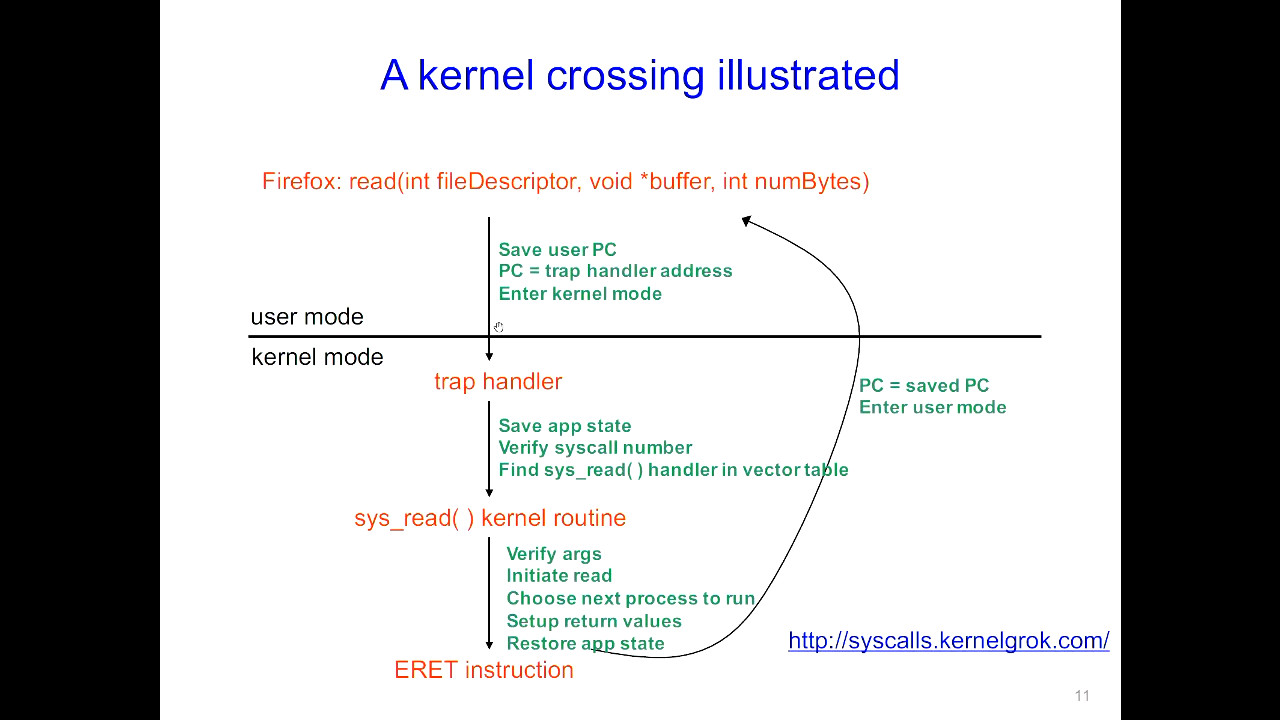
\includegraphics[height=270]{a-kernel-crossing-illustrated.jpg}
\end{center}

\textbf{System call issues}
\begin{itemize}
    \item A syscall is not a subroutine call, with the caller specifying the next PC.\
        \begin{itemize}
            \item the caller knows where the subroutines are located in memory;
                therefore they can be the target of an attack.
        \end{itemize}
    \item The kernel saves state?
        \begin{itemize}
            \item Prevents overwriting of values
        \end{itemize}
    \item The kernel verify arguments
        \begin{itemize}
            \item Prevents buggy code crashing the system
        \end{itemize}
    \item Referring to kernel objects as arguments
        \begin{itemize}
            \item Data copied between user buffer and kernel buffer.
        \end{itemize}
\end{itemize}

\textbf{Exception handling and protection}
\begin{itemize}
    \item \emph{All} entries to the OS occur via the mechanism just shown
        \begin{itemize}
            \item Acquiring privileged mode and branching to the trap handler are inseparable
        \end{itemize}
    \item Terminology
        \begin{itemize}
            \item \emph{Interrupt}: asynchronous; caused by an external device
            \item \emph{Exception}: synchronous; unexpected problem with instruction
            \item \emph{Trap}: synchronous; intended transition to OS due to an instruction
        \end{itemize}
        In all three cases, they are instances of where something strange happens,
        and the OS takes control: whether by accident, or by intention.
    \item Privileged instructions and resources are the basis for most everything:
        memory protection, protected I/O, limiting user resource consumption.
\end{itemize}

\subsection{Operating System structure}

\subsubsection{Layers}

\textbf{Operating System structure}
\begin{itemize}
    \item The OS sits between application programs and the hardware
        \begin{itemize}
            \item it mediates access and abstracts away ugliness
            \item programs request services via traps or exceptions
            \item devices request attention via interrupts
        \end{itemize}
\end{itemize}

\textbf{Operating system design and implementation}
\begin{itemize}
    \item Design and implementation of OS not ``solvable'', but some approaches have proven
        successful.
    \item Internal structure of different OS\emph{s} can vary widely.
    \item Start the design by defining goals and specifications.
    \item Affected by choice of hardware, type of system.
    \item \emph{User} goals, and \emph{system} goals
        \begin{itemize}
            \item User goals: OS should be convenient to use, easy to learn, reliable, safe,
                and fast
            \item System goals: OS should be easy to design, implement, and maintain,
                as well as flexible, reliable, error-free, and efficient.
        \end{itemize}
    \item Important principle to separate
        \begin{itemize}
            \item \textbf{Policy}: \emph{What} will be done?
            \item \textbf{Mechanism}: \emph{How} to do it?
        \end{itemize}
    \item Mechanisms determine how to do something, policies decide what will be done.
    \item The separation of policy from mechanism is a very important principle,
        it allows maximum flexibility if policy decisions are to be changed later
        (e.g.\ timer).
    \item Specifying and designing an OS is a highly creative task of
        \emph{software engineering}.
\end{itemize}

\textbf{System layers}
\begin{center}{}
    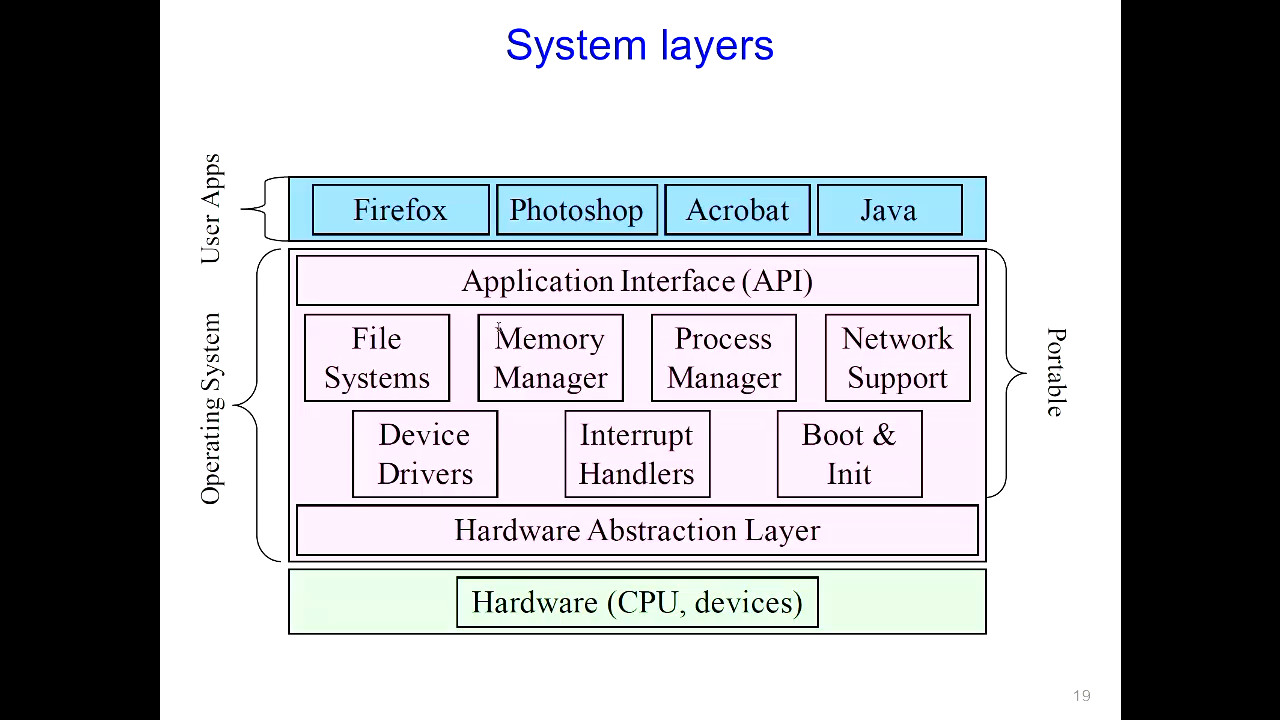
\includegraphics[height=270]{system-layers.jpg}
\end{center}

\textbf{Major OS components}
\begin{itemize}
    \item processes
    \item memory
    \item I/O
    \item secondary storage
    \item file systems
    \item protection
    \item shells
    \item GUI
    \item networking
\end{itemize}

\textbf{OS structure}

\begin{itemize}
    \item There's no clear hierarchy within an OS --- each of them needs access to different
        things.
    \item An OS consists of all these components, plus:
        \begin{itemize}
            \item many other components
            \item system programs (privileged, and non-privileged)
        \end{itemize}
    \item Major issue:
        \begin{itemize}
            \item how do we organize all this?
            \item what are all of the code modules, and where do they exist?
            \item how do they cooperate?
        \end{itemize}
    \item Massive software engineering and design problem
        \begin{itemize}
            \item design a large, complex program that:
                performs well, is reliable, is extensible, and is backwards compatible.
        \end{itemize}
\end{itemize}

\subsubsection{Examples}

\textbf{Monolithic design}
\begin{itemize}
    \item Traditionally, OS\emph{s} (like Unix) were built as a \emph{monolithic} entity
        User programs | OS (everything) | hardware
    \item Major advantage: cost of module interactions is low (procedure call)
    \item Disadvantages:
        \begin{itemize}
            \item hard to understand
            \item hard to modify
            \item unreliable (no isolation between system modules)
            \item hard to maintain
        \end{itemize}
    \item What is the alternative? \\
        Find a way to organise the OS in order to simplify its design and implementation.
\end{itemize}

\textbf{Layering}
\begin{itemize}
    \item The traditional approach is layering
        \begin{itemize}
            \item implement OS as a set of layers
            \item each layer presents an enhanced \emph{virtual machine} to the layer above
        \end{itemize}
    \item The first description of this approach was Dijkstra's THE system
        \begin{itemize}
            \item Layer 5: \emph{Job managers} execute users' programs
            \item Layer 4: \emph{Device managers} handle devices and provide buffering
            \item Layer 3: \emph{Console manager} implements virtual consoles
            \item Layer 2: \emph{Page manager} implements virtual memories for each process
            \item Layer 1: \emph{Kernel} implements a virtual processor for each process
            \item Layer 0: \emph{Hardware}
        \end{itemize}
    \item Each layer can be tested and verified independently
    \item Imposes a hierarchical stricture
        \begin{itemize}
            \item but real systems are more complex:
                file systems require VM services (buffer);
                VM would like to use files for its backing store
            \item strict layering isn't flexible enough
        \end{itemize}
    \item Poor performance:
        each layer crossing has \emph{overhead} associated with it
    \item Disjunction between model and reality:
        systems modelled as layers, but not really built that way.
\end{itemize}

\textbf{Hardware abstraction layer}
\begin{itemize}
    \item An example of layering in modern operating systems
    \item Goal: separates hardware-specific routines from the \emph{core} OS
        \begin{itemize}
            \item Provides portability
            \item Improves readability
        \end{itemize}
\end{itemize}

\textbf{Microkernels}
\begin{itemize}
    \item Popular in the late 80s, early 90s
    \item Goal:
        minimize what happens in kernel;
        item organize rest of OS as user-level processes.
    \item This results in:
        \begin{itemize}
            \item better reliability (isolation between components)
            \item easy of extension and customisation
            \item poor performance (user/kernel boundary crossings)
        \end{itemize}
    \item First microkernel system was Hydra (CMU, 1970)
        \begin{itemize}
            \item Contemporaries: Mach (CMU), Chorus (French Unix-like OS), OS X (Apple),
                in some ways NT (Microsoft)
        \end{itemize}
\end{itemize}

\begin{center}{}
    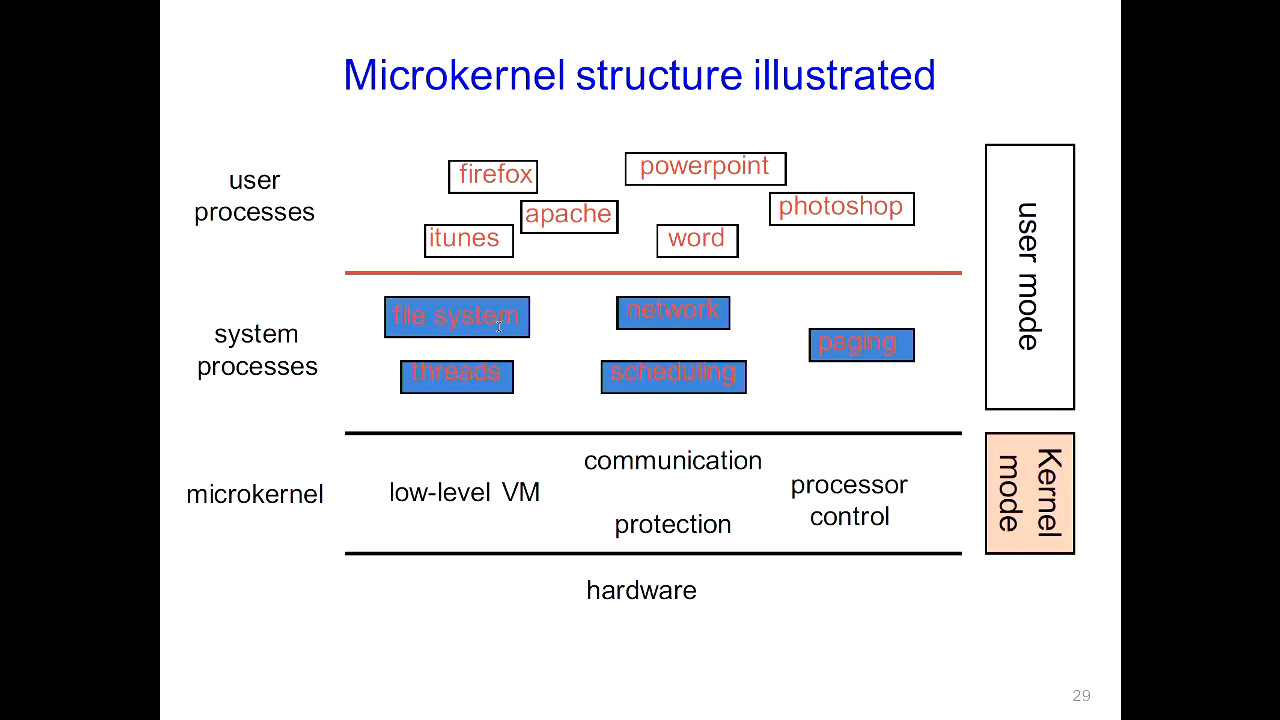
\includegraphics[height=270]{microkernel-structure-illustrated.jpg}
\end{center}

\textbf{Comparison of OS structures}

Windows

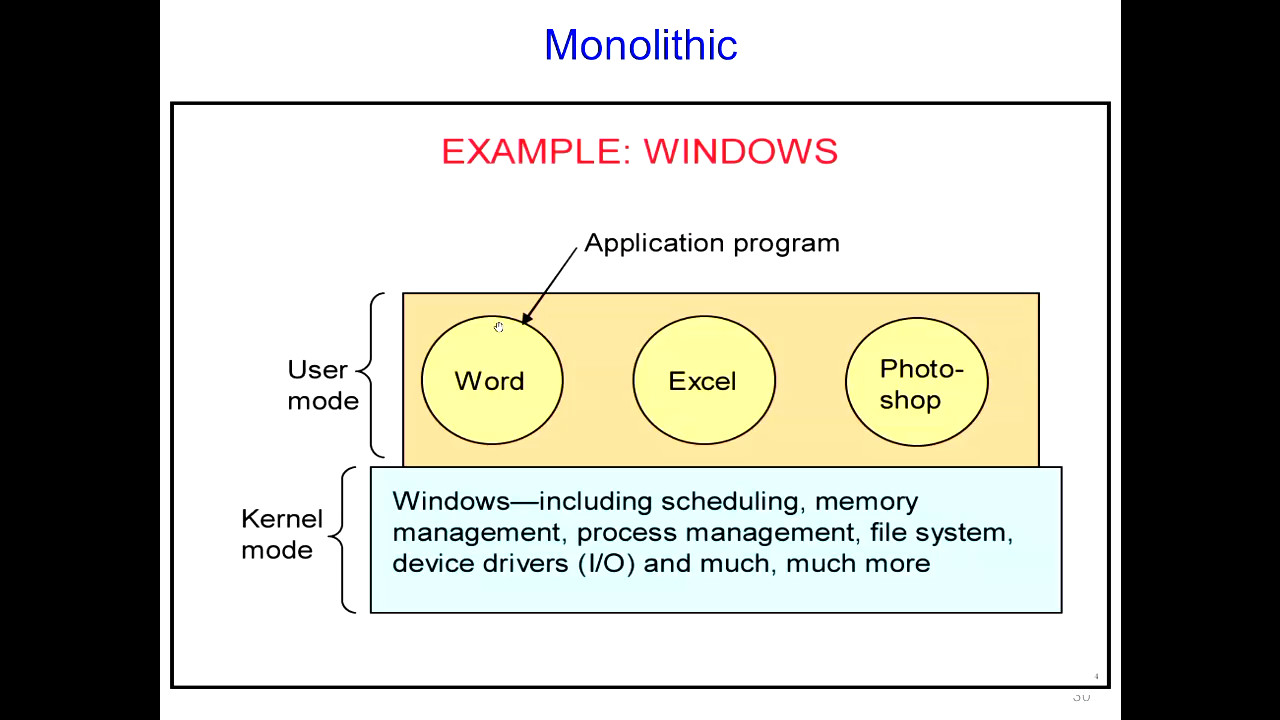
\includegraphics[height=270]{windows.jpg}

MINIX 3

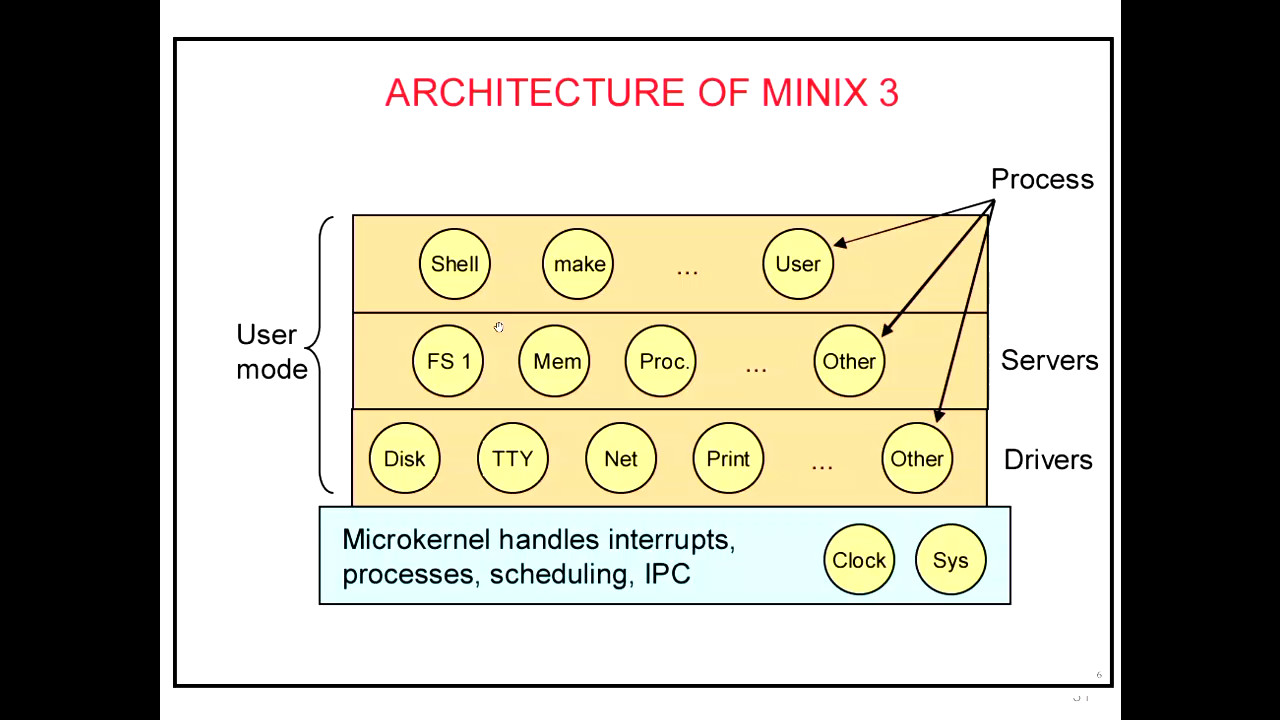
\includegraphics[height=270]{minix-3.jpg}

\textbf{Loadable kernel modules}

\begin{itemize}
    \item (Perhaps) the best practice for OS design
    \item Core services in the kernel, and others dynamically loaded
    \item Common implementations include: Solaris, Linux, etc.
    \item Advantages
        \begin{itemize}
            \item convenient: no need for rebooting for newly added modules
            \item efficient: no need for message passing unlike micro-kernel
            \item flexible: any module can call any other module unlike layered model
        \end{itemize}
\end{itemize}

\subsection{Summary}

\begin{itemize}
    \item Fundamental distinction between user and privileged mode supported by most hardware
    \item OS design has been an evolutionary process of trial and error.
    \item Successful OS designs have run the spectrum  from monolithic, to layered,
        to micro-kernels
    \item The role and design of an OS are still evolving
    \item It is impossible to pick one ``correct'' way to structure an OS
\end{itemize}

\break{}

\section{Processes}

\subsection{Process}

\textbf{What is a ``process''?}
\begin{itemize}
    \item The process is the OS\emph{s} abstraction for execution
        \begin{itemize}
            \item A process is a program in execution
        \end{itemize}
    \item Simplest (classic) case: a \emph{sequential process}
        \begin{itemize}
            \item An address space (an abstraction of memory)
            \item A single thread of execution (an abstraction of the CPU)
        \end{itemize}
    \item A sequential process is:
        \begin{itemize}
            \item The unit of execution
            \item The unit of scheduling
            \item The dynamic (active) execution context
                (as opposed to the program --- static, just a bunch of bytes)
        \end{itemize}

\end{itemize}

\textbf{What's ``in'' a process?}
\begin{itemize}
    \item A process consists of (at least):
        \begin{itemize}
            \item An \emph{address space}, containing:
                \begin{itemize}
                    \item the code (instructions) for the running program
                    \item the data for the running program (static data, heap data, stack)
                \end{itemize}
            \item \emph{CPU state}, consisting of:
                \begin{itemize}
                    \item the program counter (PC), indicating the next instruction;
                    \item the stack pointer;
                    \item other general purpose register values.
                \end{itemize}
            \item A set of \emph{OS resources}
                \begin{itemize}
                    \item open files, network connections, sound channels, \dots
                \end{itemize}
            \item In other words, everything needed to run the program
                (or to restart, if interrupted).
        \end{itemize}
\end{itemize}

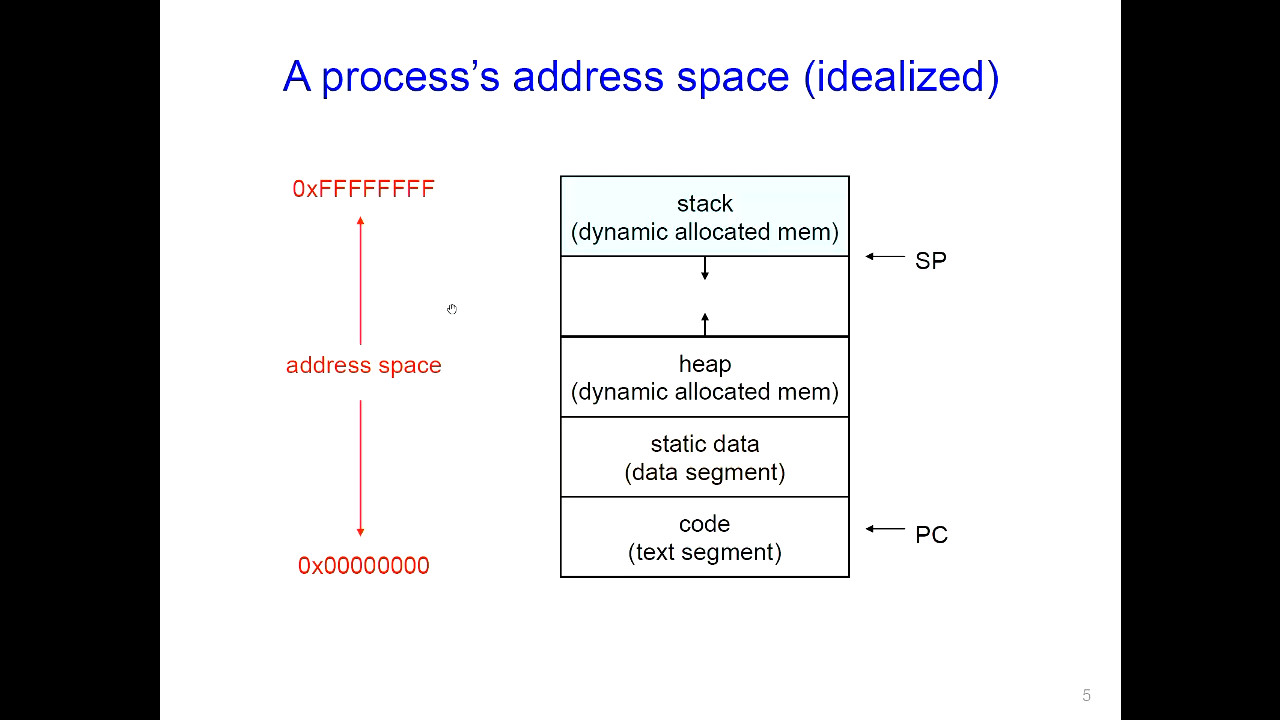
\includegraphics[height=270]{a-process-address-space.jpg}

\textbf{The OS process namespace}
\begin{itemize}
    \item The particulars depend on the specific OS, but the principles are general;
    \item The name for a process is called a \emph{process ID} (PID) (an integer);
    \item The PID namespace is global to the system;
    \item Operations that create processes return a PID (e.g.\ fork);
    \item Operations on processes take PIDs as an argument (e.g.\ kill, wait, nice).\
\end{itemize}

\subsection{Process control block}

\textbf{Representation of processes by the OS}
\begin{itemize}
    \item The OS maintains a data structure to keep track of a process's state
        \begin{itemize}
            \item called the \emph{process control block} (PCB)
                or \emph{process descriptor};
            \item identified by the PID.\
        \end{itemize}
    \item OS keeps all of a process's execution state in (or linked from) the PCB
        when the process isn't running
        \begin{itemize}
            \item PC, SP, registers, etc.
            \item when a process is unscheduled, the state is transferred out of the
                hardware into the PCB
            \item (when a process is running, its state is spread between the PCB and the CPU).
        \end{itemize}
\end{itemize}

\textbf{The PCB}
\begin{itemize}
    \item The PCB is a data structure with many, many fields
        \begin{itemize}
            \item PID
            \item parent PID
            \item execution state
            \item PC, SP, registers
            \item address space info
            \item Unix user id, group id
            \item scheduling priority
            \item accounting info
            \item pointers for state queues
        \end{itemize}
    \item In Linux:
        \begin{itemize}
            \item defined in \texttt{task\_struct (include/linux/sched.h)}
            \item Over 95 fields!
        \end{itemize}
\end{itemize}

\subsection{Process state \& context switch}

\textbf{PCBs and CPU state}
\begin{itemize}
    \item When a process is running, its CPU state is inside the CPU
        \begin{itemize}
            \item PC, SP, registers
            \item CPU contains current values
        \end{itemize}
    \item When the OS gets control because of a
        \begin{itemize}
            \item \emph{Trap}: program executes a syscall
            \item \emph{Exception}: program does something unexpected (e.g.\ page fault)
            \item \emph{Interrupt}: A hardware device requests service
        \end{itemize}
        the OS saves the CPU state of the running process in that process's PCB.\

    \item When the OS returns the process to the running state
        \begin{itemize}
            \item it loads the hardware registers with values from that process's PCB
            \item e.g.\ general purpose registers, SP, instruction pointer
        \end{itemize}
    \item This act of switching the CPU from one process to another is called a
        \emph{context switch}
        \begin{itemize}
            \item systems may do 100s or 1000s of switches per second;
            \item takes a few microseconds on today's hardware;
            \item still expensive relative to thread-based context switches.\
        \end{itemize}
    \item Choosing which process to run next is called \emph{scheduling}.\
\end{itemize}

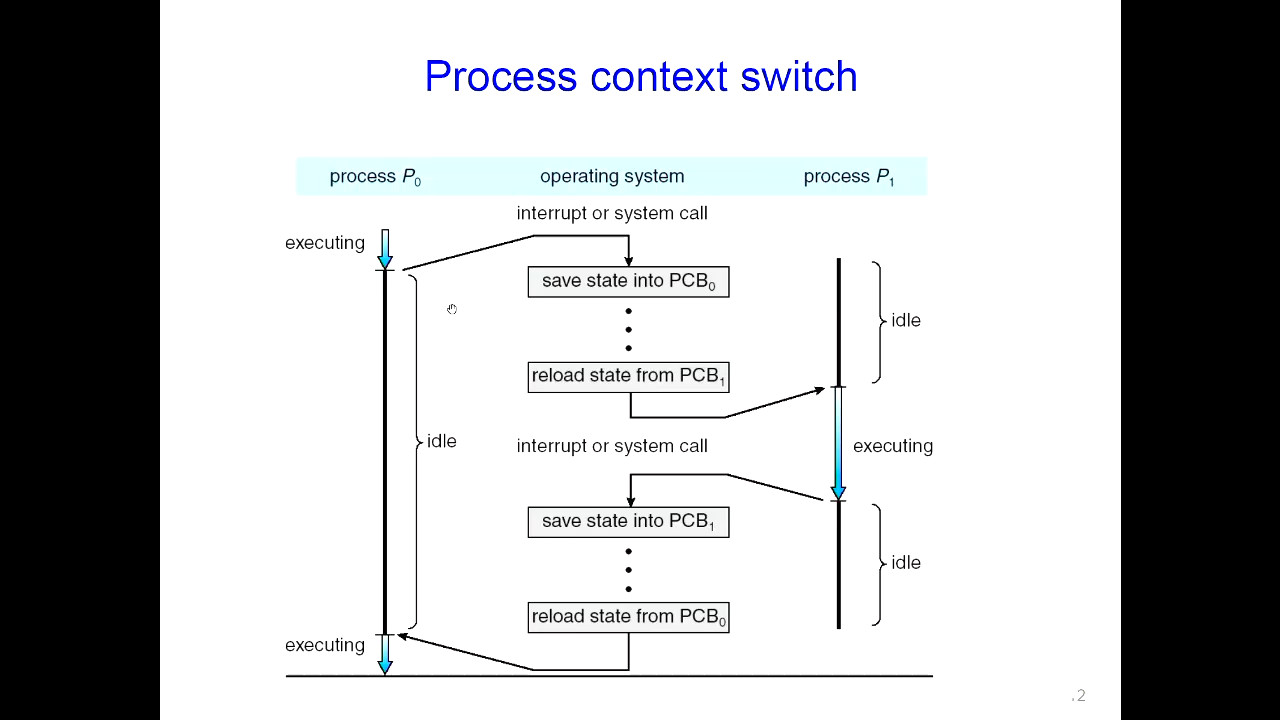
\includegraphics[height=270]{process-context-switch.jpg}

\textbf{Process execution states}
\begin{itemize}
    \item Each process has an \emph{execution state}, which indicates what it's currently doing
        \begin{itemize}
            \item \emph{ready}: waiting to be assigned to a CPU ---
                could run, but another process has the CPU;\
            \item \emph{running}: executing on a CPU ---
                it's the process that currently controls the CPU;\
            \item \emph{waiting} (aka ``blocked''): waiting for an event, e.g.\ I/O completion,
                or a messing from (or the completion of) another process ---
                cannot make progress until the event happens.
        \end{itemize}
    \item As a process executes, it moves from state to state
        \begin{itemize}
            \item Unix:\ run \texttt{top}, STAT column shows current state
            \item which state is a process most of the time?
        \end{itemize}
\end{itemize}

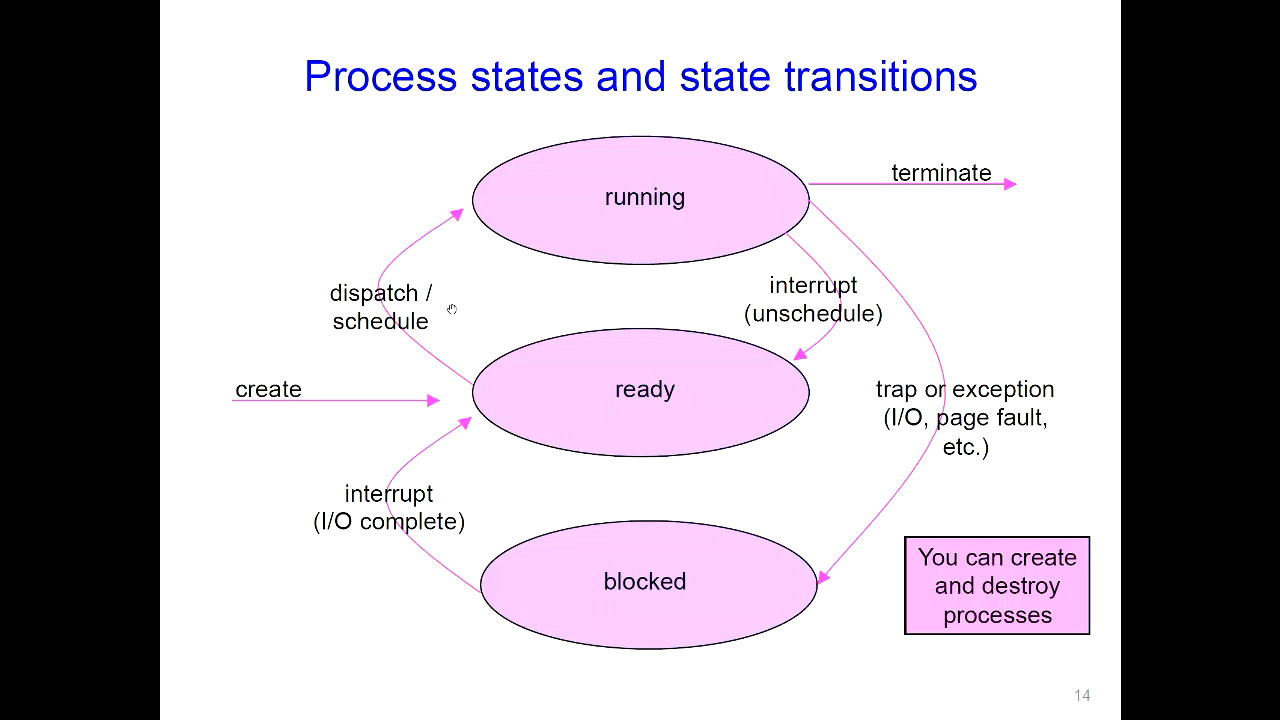
\includegraphics[height=270]{process-states-and-state-transitions.jpg}

\textbf{State queues}
\begin{itemize}
    \item The OS maintains a collection of queues that represent the state of all processes in
        the system
        \begin{itemize}
            \item typically one queue for each state (e.g.\ ready, waiting, \dots);
            \item each PCB is queued onto a state queue according to the current state of the
                process it represents;
            \item as a process changes state, its PCB is unlinked from one queue,
                and linked onto another.
        \end{itemize}
    \item The PCBs are moved between queues, which are represented as linked lists.
    \item There may be many wait queues, one for each type of wait
        (particular device, timer, message, \dots).
\end{itemize}

\textbf{PCBs and state queues}
\begin{itemize}
    \item PCBs are data structures
        \begin{itemize}
            \item dynamically allocated inside OS memory.
        \end{itemize}
    \item When a process is created:
        \begin{itemize}
            \item OS allocates a PCB for it;
            \item OS initializes PCB;\
            \item (OS does other things not related to the PCB);
            \item OS puts PCB on the correct queue.
        \end{itemize}
    \item As a process computes:
        \begin{itemize}
            \item OS moves its PCB from queue to queue.
        \end{itemize}
    \item When a process is terminated:
        \begin{itemize}
            \item PCB may be retained for a while (to receive signals, etc.)
            \item eventually, OS deallocates the PCB.\
        \end{itemize}
\end{itemize}

\subsection{Process creation and termination}

\textbf{Process creation}
\begin{itemize}
    \item New processes are created by existing processes
        \begin{itemize}
            \item creator is called the \emph{parent};
            \item created process is called the \emph{child};\\\
                Unix:\ do \texttt{ps -ef}, look for PPID field
            \item what creates the first process, and when? \\
                on Unix, this first process is init; \\
                on many Linux distributions, this is SystemD or Runit (on Void).
        \end{itemize}
\end{itemize}

\textbf{Process creation semantics}
\begin{itemize}
    \item (Depending on the OS) child processes inherit certain attributes of the parent.
        E.g.
        \begin{itemize}
            \item Open file table: implies \texttt{stdin}/\texttt{stdout}/\texttt{stderr};
            \item On some systems, resource allocation to parent may be divided among children.
        \end{itemize}
    \item (In Unix) when a child is created, the parent may either wait for the child to
        finish, or continue in parallel.
\end{itemize}

\textbf{Unix process creation details}
\begin{itemize}
    \item Unix process creation through \texttt{fork} system call
        \begin{itemize}
            \item creates and initializes a new PCB
                \begin{itemize}
                    \item initializes kernel resources of new process with resources of parent
                        (e.g.\ open files)
                    \item initializes PC, SP to be same as parent.
                \end{itemize}
            \item creates a new address space
                \begin{itemize}
                    \item initialises new address space with a copy of the entire contents of
                        the address space of the parent
                \end{itemize}
            \item places new PCB on the ready queue.
        \end{itemize}
    \item the \texttt{fork} system call ``returns twice''
        \begin{itemize}
            \item once into the parent, and once into the child
                \begin{itemize}
                    \item returns the child's PID to the parent
                    \item returns \texttt{0} to the child
                \end{itemize}
        \end{itemize}
    \item \texttt{fork} = ``clone me''. \\
        The return value is used to determine whether we're the clone or the original.
\end{itemize}

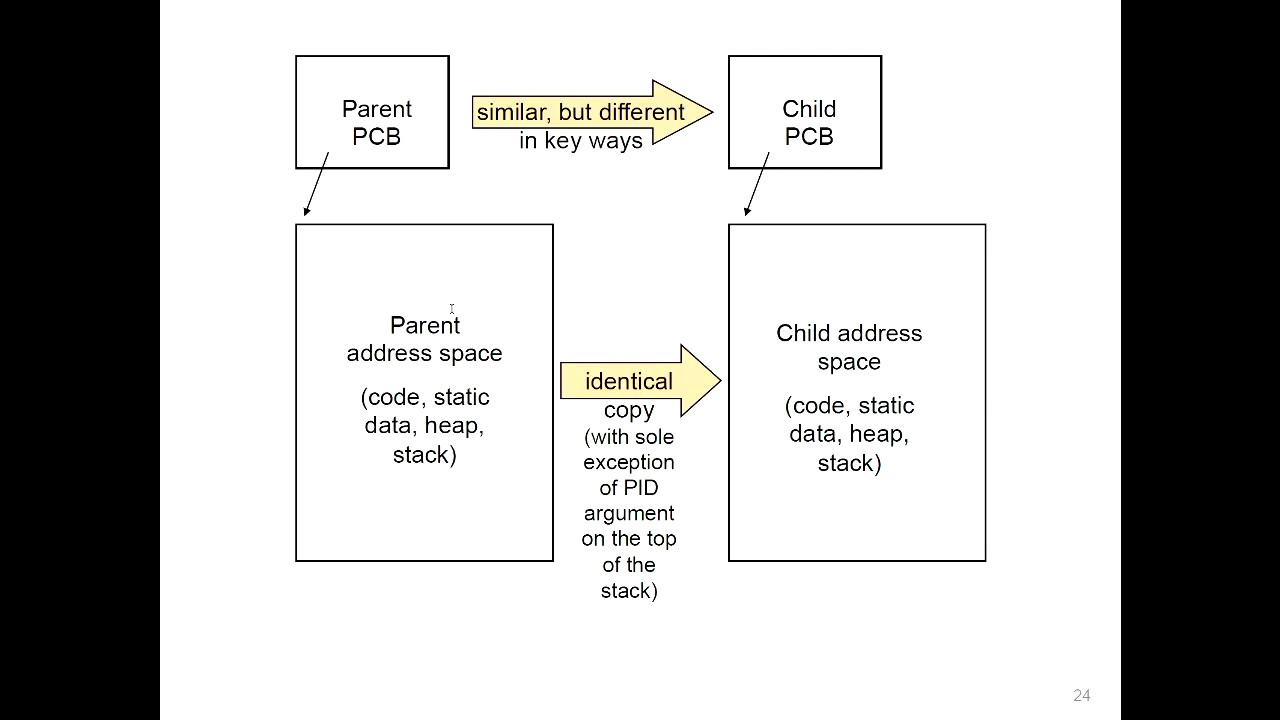
\includegraphics[height=270]{fork.jpg}

\textbf{\texttt{exec} v.s.\ \texttt{fork}}
\begin{itemize}
    \item Q:\ So how do we start a new program, instead of just forking the old program?
    \item A:\ First \texttt{fork}, then \texttt{exec}.
    \item \texttt{exec}
        \begin{itemize}
            \item stops the current process
            \item loads program `prog' into the address space
                (i.e.\ overwrites the existing process image)
            \item initialises hardware context, args for new program
            \item places PCB onto ready queue
            \item \emph{does not create a new process!}
        \end{itemize}
\end{itemize}

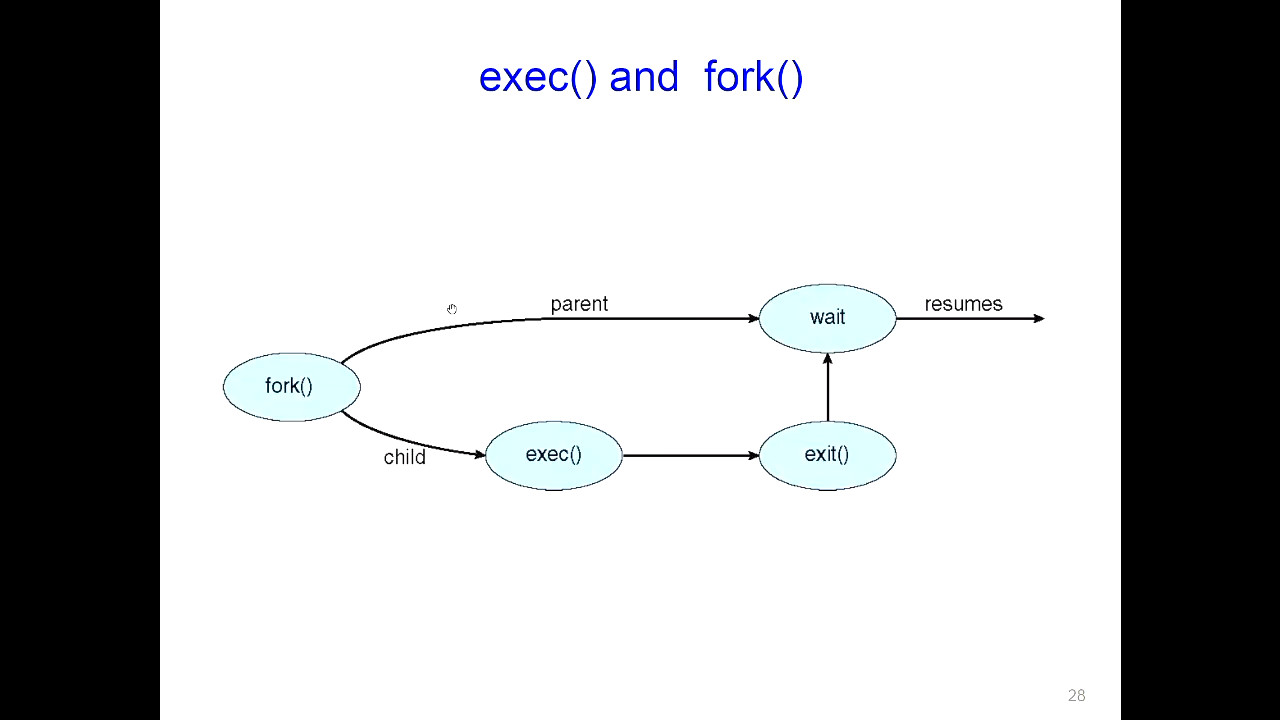
\includegraphics[height=270]{exec-and-fork.jpg}

\textbf{Method 1: \texttt{vfork}}
\begin{itemize}
    \item \texttt{vfork} is the older (now uncommon) of the two approaches.
    \item Instead of ``child's address space is a copy of the parent's'',
        the semantics are ``child's address space \emph{is} the parent's'',
        \begin{itemize}
            \item with a ``promise'' that the child won't modify the address space before doing
                an \texttt{execve}.
            \item When \texttt{execve} is called, a new address space is created and it's
                loaded with the new executable.
            \item Parent is blocked until \texttt{execve} is executed by child.
            \item Saves wasted effort of duplicating parent's address space.
        \end{itemize}
\end{itemize}

\textbf{Method 2: copy-on-write}
\begin{itemize}
    \item Retains the original semantics, but copies ``only what is necessary'' rather than
        the entire address space.
    \item On \texttt{fork}:
        \begin{itemize}
            \item Create a new address space
            \item Initialise page tables with same mappings as the parent's
                (i.e.\ they both point to the same physical memory).
                \begin{itemize}
                    \item (No copying of address space contents have occurred at this point
                        --- with the sole exception of the top page of the stack.)
                \end{itemize}
            \item Set both parent and child page tables to make all pages read-only
            \item If either parent or child writes to memory, an exception occurs.
            \item When exception occurs, OS copies the page, adjusts page tables, etc.
        \end{itemize}
\end{itemize}

\subsection{Summary}
\begin{itemize}
    \item Process
    \item PCB
    \item Process state
    \item Context switch
    \item Process creation and termination
\end{itemize}

\break{}

\section{Threads}

\subsection{Process vs Threads}

\textbf{What's \emph{in} a process?}
\begin{itemize}
    \item A process consists of (at least):
        \begin{itemize}
            \item An \emph{address space}, containing
                \begin{itemize}
                    \item the code (instructions) for the running program
                    \item the data for the running program
                \end{itemize}
            \item \emph{Thread state}, consisting of
                \begin{itemize}
                    \item The PC, indicating the next instruction
                    \item The SP, indicating the position on the stack
                    \item Other general purpose registers
                \end{itemize}
            \item A set of \emph{OS resources}
                \begin{itemize}
                    \item Open files, network connections, sound channels, \dots
                \end{itemize}
        \end{itemize}
    \item Decompose \dots
        \begin{itemize}
            \item address space
            \item \emph{thread of control} (stack, SP, PC, registers)
            \item OS resources
        \end{itemize}
\end{itemize}

\textbf{Motivation}
\begin{itemize}
    \item Threads are about \emph{concurrency} and \emph{parallelism}
    \item One way to get concurrency and parallelism is to use multiple processes
        \begin{itemize}
            \item The programs (code) of distinct processes are isolated from each other
        \end{itemize}
    \item Threads are another way to get concurrency and parallelism
        \begin{itemize}
            \item Threads \emph{share a process} --- same address space, same OS resources
            \item Threads have private stack, CPU state --- are schedulable
        \end{itemize}
\end{itemize}

\textbf{What's needed?}
\begin{itemize}
    \item In many cases
        \begin{itemize}
            \item Everybody wants to run the same code
            \item Everybody wants to access the same data
            \item Everybody has the same privileges
            \item Everybody uses the same resources (open files, network connections, etc.)
        \end{itemize}
    \item But you'd like to have multiple hardware execution states:
        \begin{itemize}
            \item an execution stack and SP
                \begin{itemize}
                    \item traces state of procedure calls made
                \end{itemize}
            \item the PC, indicating the next instruction
            \item a set of general-purpose processor registers and their values
        \end{itemize}
\end{itemize}

\textbf{How could we achieve this?}
\begin{itemize}
    \item Given the process abstraction as we know it:
        \begin{itemize}
            \item for several processes
            \item cause each to \emph{map} to the \emph{same} physical memory to share data
                (\texttt{shmget}),
        \end{itemize}
    \item This is really inefficient
        \begin{itemize}
            \item space: PCB, page tables, etc.
            \item time: creating OS structures, fork/copy address space, etc.
        \end{itemize}
\end{itemize}

\textbf{Can we do better?}
\begin{itemize}
    \item Key idea:
        \begin{itemize}
            \item separate the concept of a \emph{process} (address space, OS resources)
            \item \dots from that of a minimal \emph{thread of control}
                (execution state: stack, SP, PC, registers),
        \end{itemize}
    \item This execution state is usually called a \emph{thread}, or a
        \emph{lightweight process}.
\end{itemize}

\textbf{Threads and processes}
\begin{itemize}
    \item Most modern OS\emph{s} support two entities:
        \begin{itemize}
            \item the \emph{process}, which defines the address space and general process
                attributes (such as open files, etc.)
            \item the \emph{thread}, which defines a sequential execution stream within a
                process.
        \end{itemize}
    \item A thread is bound to a single process / address space
        \begin{itemize}
            \item address spaces, however, can have multiple threads executing within them
            \item sharing data between threads is cheap: all see the same address space
            \item creating threads is cheap, too!
        \end{itemize}
    \item \emph{Threads become the unit of scheduling}
        \begin{itemize}
            \item processes / address spaces are just \emph{containers} in which threads
                execute.
        \end{itemize}
\end{itemize}

\textbf{Single and Multi-threaded Processes}
\begin{itemize}
    \item Different threads in the same process have separate registers and stacks.
    \item This is cheaper than duplicating the instructions and PCB etc.,
        as required by having multiple processes.
\end{itemize}

\subsection{Concurrency}

\textbf{Communication}
\begin{itemize}
    \item Threads are concurrent executions sharing an address space (and some OS resources)
    \item Address spaces provide isolation
        \begin{itemize}
            \item If you can't name an object, you can't read or write to it
        \end{itemize}
    \item Hence, communicating between processes is expensive
        \begin{itemize}
            \item Must go through the OS to move data from one address space to another
        \end{itemize}
    \item Because threads are in the same address space, communication is simple/cheap
        \begin{itemize}
            \item Just update a shared variable!
        \end{itemize}
\end{itemize}

\textbf{The design space}

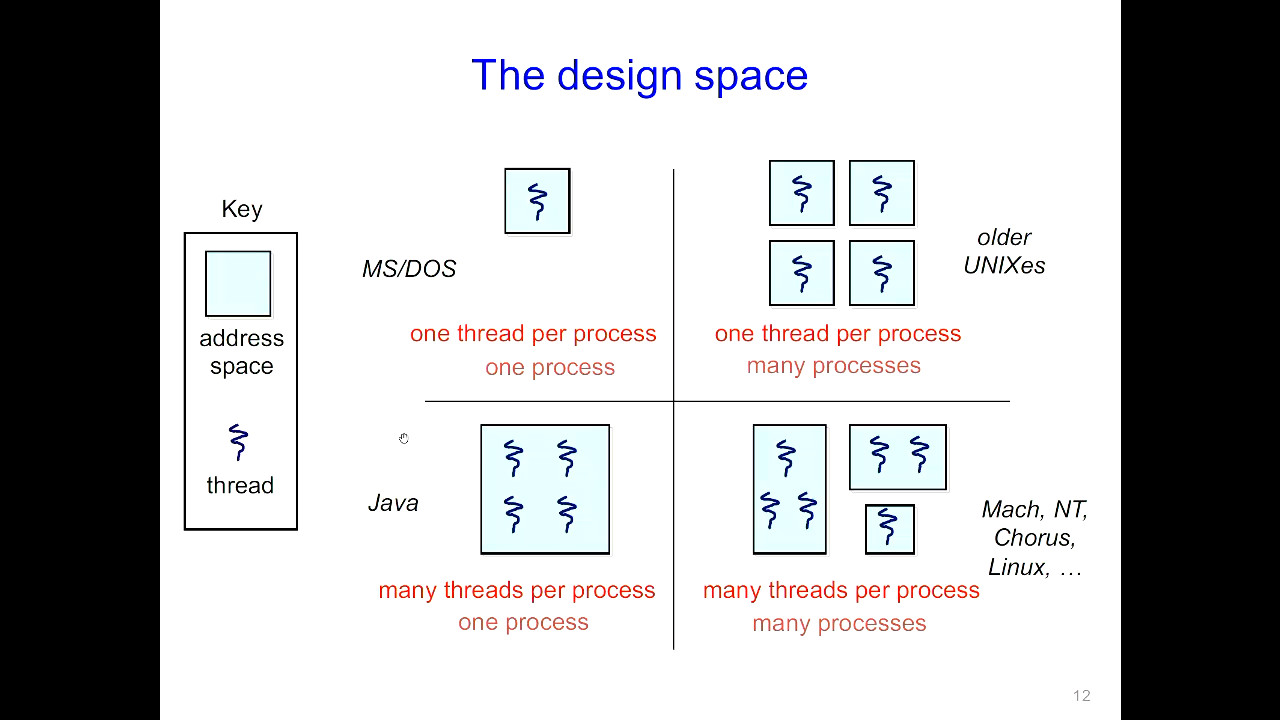
\includegraphics[height=270]{the-design-space.jpg}

\textbf{Process address space}

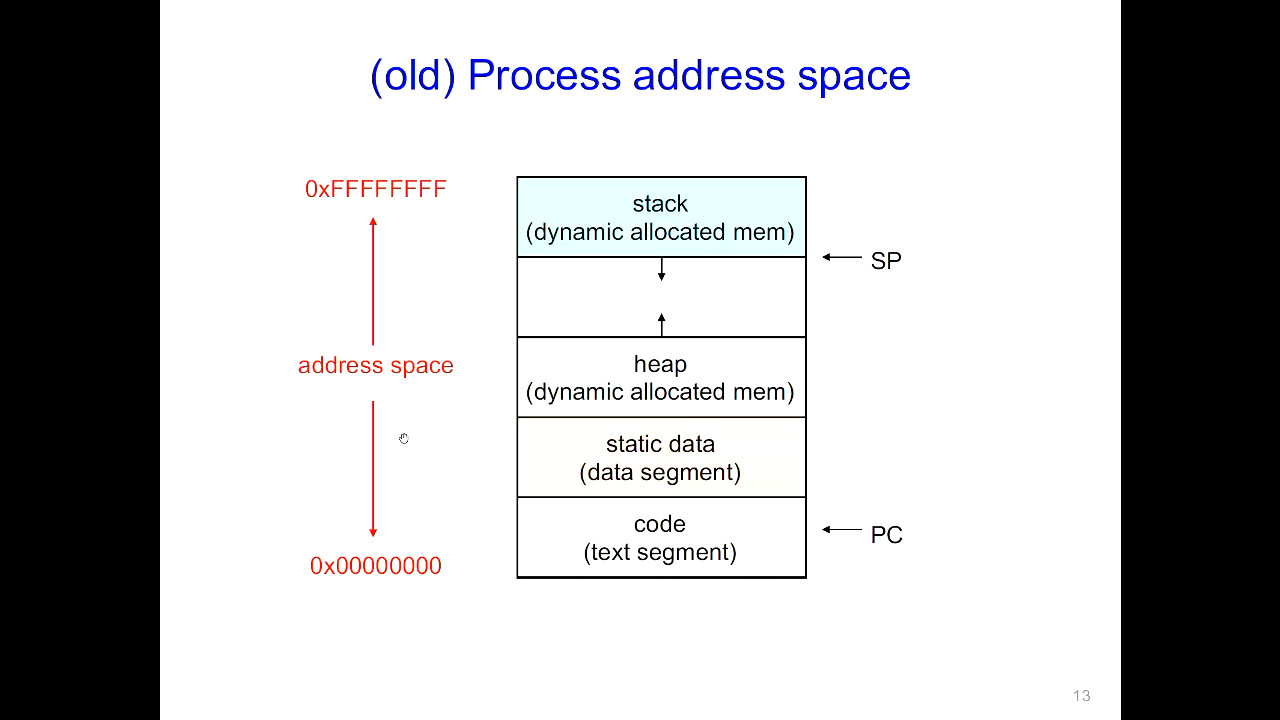
\includegraphics[height=270]{process-address-space.jpg}

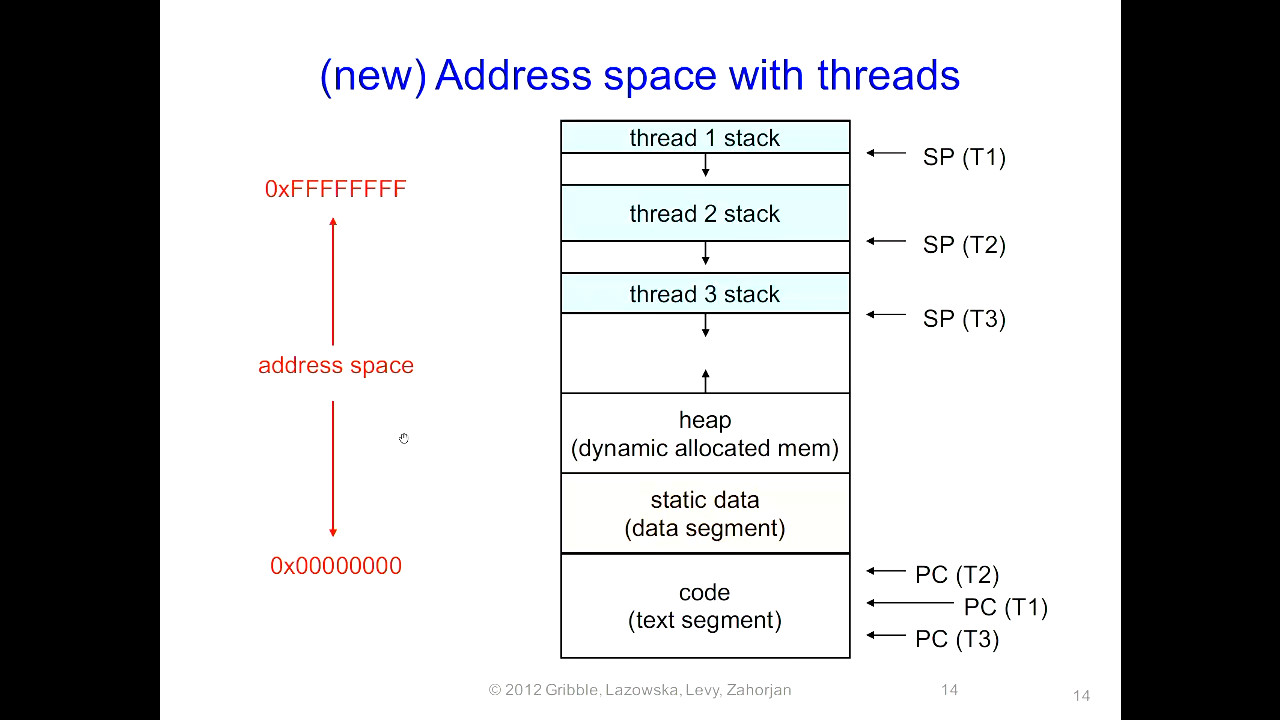
\includegraphics[height=270]{process-address-space-threads.jpg}

\subsection{Design space of process/threads}

\textbf{Process/thread separation}
\begin{itemize}
    \item Concurrency (multi-threading) is useful for:
        \begin{itemize}
            \item handling concurrent events (e.g.\ web servers and clients)
            \item building parallel programs (e.g.\ matrix multiply, ray tracing)
            \item improving program structure (the Java argument),
        \end{itemize}
    \item Multi-threading is useful even on a uniprocessor
        \begin{itemize}
            \item even though only one thread can run at a time
        \end{itemize}
    \item Supporting multi-threading --- that is, separating the concept of a \emph{process}
        (address space, files, etc.) from that of a minimal \emph{thread of control}
        (execution state), is a big win
        \begin{itemize}
            \item creating concurrency does not require creating new processes
            \item ``faster / better / cheaper''
        \end{itemize}
\end{itemize}

\subsection{Kernel threads}

\textbf{Where do threads come from?}
\begin{itemize}
    \item Natural answer: the OS is responsible for creating/managing threads \\
        For example, the kernel call to create a new thread would
        \begin{itemize}
            \item allocate an execution stack within the process address space
            \item create and initialize a \emph{Thread Control block} \\
                (SP, PC, register values)
            \item stick it on the ready queue
        \end{itemize}
    \item We call these \emph{kernel threads} \\
        There is a ``thread name space''
        \begin{itemize}
            \item Thread IDs (TIDs)
            \item TIDs are integers
        \end{itemize}
\end{itemize}

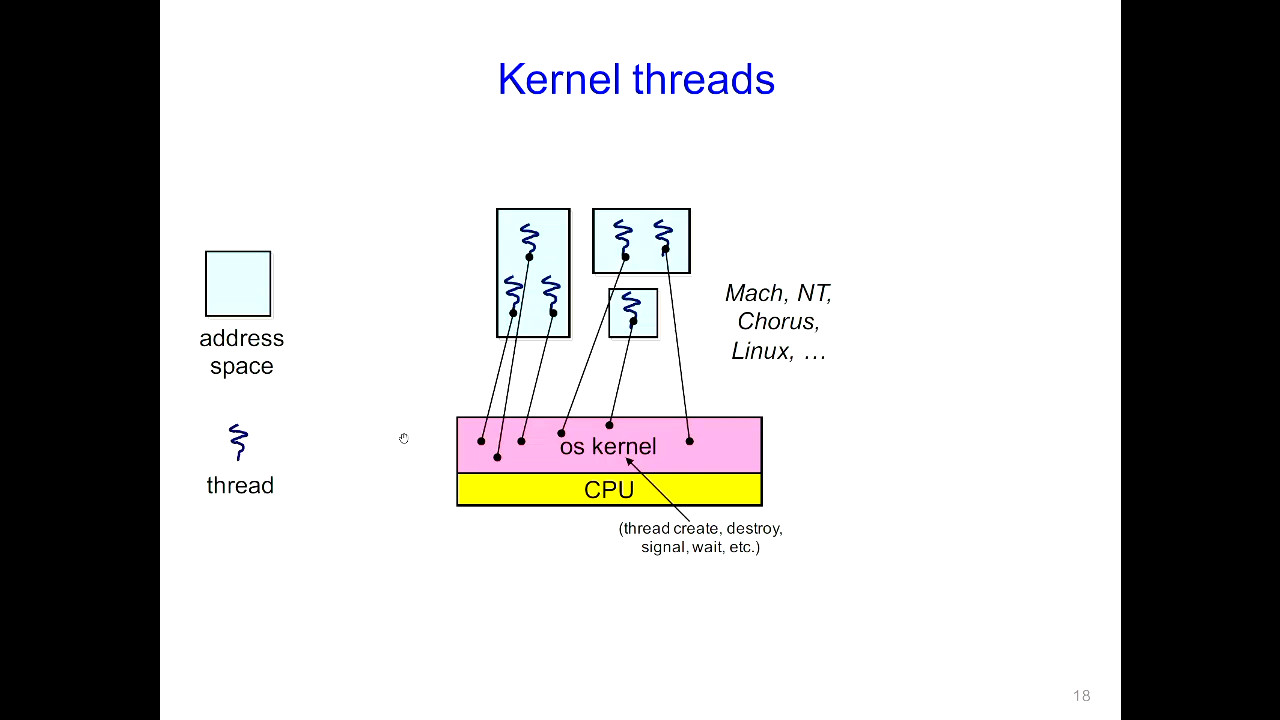
\includegraphics[height=270]{kernel-threads.jpg}

\textbf{Kernel Threads}
\begin{itemize}
    \item OS now manages threads \emph{and} processes / address spaces
        \begin{itemize}
            \item all thread operations are implemented in the kernel
            \item OS schedules all of the threads in a system
                \begin{itemize}
                    \item if one thread in a process blocks (e.g.\ on I/O),
                        the OS knows about it, and can run other threads from that process
                    \item possible to overlap I/O and computation \emph{inside} a process
                \end{itemize}
        \end{itemize}
    \item Kernel threads are cheaper than processes
        \begin{itemize}
            \item less state to allocate and initialise
        \end{itemize}
    \item But, they're still pretty expensive for fine-grained use
        \begin{itemize}
            \item orders of magnitude more expensive than a procedure call
            \item thread operations are all \emph{system calls}
                \begin{itemize}
                    \item context switch
                    \item argument checks
                \end{itemize}
            \item must maintain kernel state for each thread
        \end{itemize}
\end{itemize}

\subsection{User-level threads}

\textbf{Cheaper alternative}
\begin{itemize}
    \item There is an alternative to kernel threads
    \item Threads can also be managed at the user level (within the process)
        \begin{itemize}
            \item a library linked into the program manages the threads
                \begin{itemize}
                    \item the thread manager doesn't need to manipulate address spaces
                        (which only the kernel can do)
                    \item threads differ (roughly) only in hardware contexts
                        (PC, SP, registers), which can be manipulated by user-level code
                    \item the \emph{thread package} multiplexes user-level threads on top
                        of kernel threads
                    \item each kernel thread is treated as a \emph{virtual processor}
                \end{itemize}
            \item we call these \emph{user-level threads}
        \end{itemize}
\end{itemize}

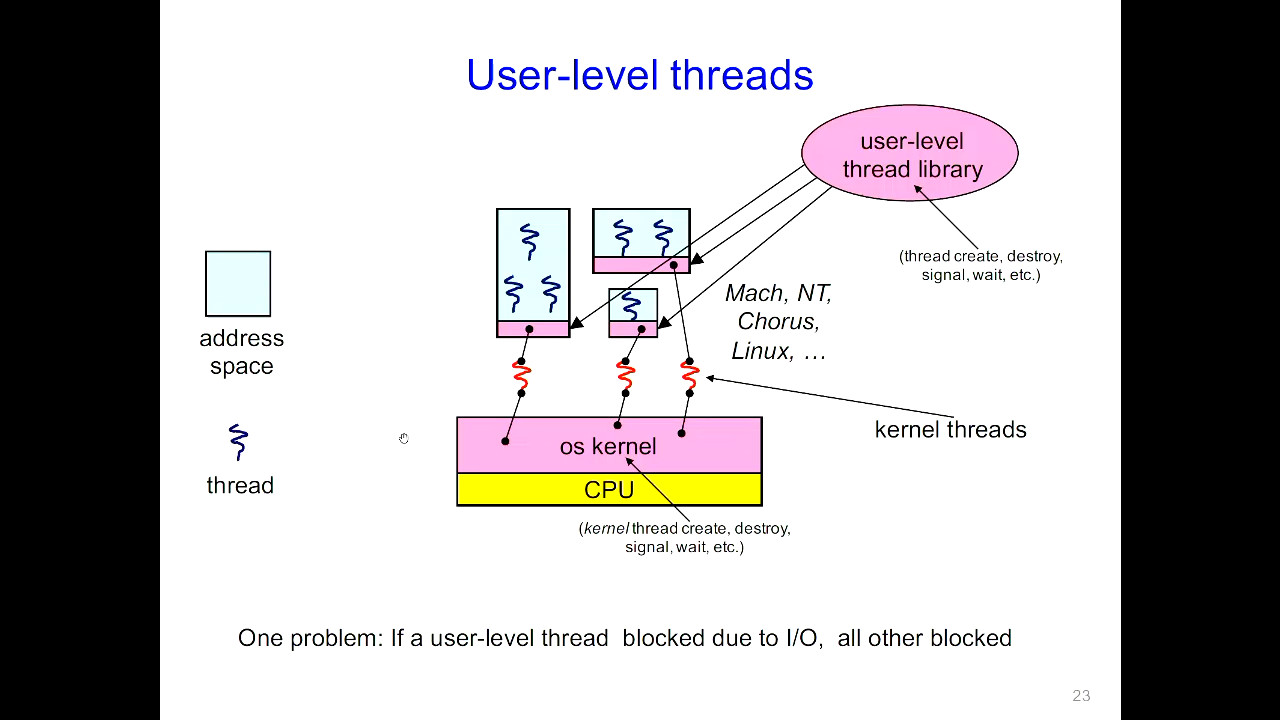
\includegraphics[height=270]{user-level-threads.jpg}

\textbf{User-level threads}
\begin{itemize}
    \item User-level threads are small and fast
        \begin{itemize}
            \item managed entirely by user-level library (e.g.\ \texttt{pthreads})
            \item each thread is represented by a PC, registers, a stack, and a small
                \emph{thread control block} (TCB)
            \item creating a thread, switching between threads, and synchronising
                threads are done \emph{via procedure calls}
                \begin{itemize}
                    \item no kernel involvement necessary!
                \end{itemize}
        \end{itemize}
    \item User-level thread operations can be 10--100x faster than kernel threads as a result.
\end{itemize}

\textbf{User-level thread implementation}
\begin{itemize}
    \item The OS schedules the kernel thread
    \item The kernel thread executes user code, including the thread support library
        and its associated thread scheduler
    \item The thread scheduler determines when a user-level thread runs
        \begin{itemize}
            \item it uses queues to keep track of what threads are doing: run, ready, wait
                \begin{itemize}
                    \item just like the OS and processes
                    \item but, implemented at user-level as a library
                \end{itemize}
        \end{itemize}
\end{itemize}

\textbf{Thread context switch}
\begin{itemize}
    \item Very simple for user-level threads:
        \begin{itemize}
            \item save context of currently running thread
                \begin{itemize}
                    \item push CPU state onto thread stack
                \end{itemize}
            \item restore context of the next thread
                \begin{itemize}
                    \item pop CPU state from next thread's stack
                \end{itemize}
            \item return as the new thread
                \begin{itemize}
                    \item execution resume at PC of next thread
                \end{itemize}
            \item Note: no changes to memory mapping required
        \end{itemize}
    \item This is all done in assembly language
        \begin{itemize}
            \item it works at the level of the procedure calling convention
        \end{itemize}
\end{itemize}

\textbf{How to keep a user-level thread from hogging the CPU?}
\begin{itemize}
    \item Strategy 1: force everyone to cooperate
        \begin{itemize}
            \item a thread willingly gives up the CPU by calling \texttt{yield}
            \item \texttt{yield} calls into the scheduler, which context switches to
                another ready thread
            \item what happens if a thread never calls \texttt{yield}?
        \end{itemize}
    \item Strategy 2: use presumption
        \begin{itemize}
            \item scheduler requests that a timer interrupt be delivered by the OS
                periodically
                \begin{itemize}
                    \item usually delivered as a Unix signal (\texttt{man signal})
                    \item signals are just like software interrupts, but delivered to
                        user-level by the OS instead of delivered to the OS by hardware
                \end{itemize}
            \item at each timer interrupt, scheduler gains control and context switches
                as appropriate.
        \end{itemize}
\end{itemize}

\textbf{What if a thread tries to do I/O}
\begin{itemize}
    \item The kernel thread ``powering'' it is lost for the duration of (synchronous)
        I/O operation!
        \begin{itemize}
            \item The kernel thread blocks in the OS, as always
            \item It maroons with it the state of the user-level thread
        \end{itemize}
    \item Could have one kernel thread ``powering'' each user-level thread
        \begin{itemize}
            \item ``common case'' operations (e.g.\ synchronisation) would be quick
        \end{itemize}
    \item Could have a limited-size ``pool'' of kernel threads ``powering'' all the
        user-level threads in the address space
        \begin{itemize}
            \item the kernel will be scheduling these threads, obliviously to what's going
                on at user-level.
        \end{itemize}
\end{itemize}

\subsection{Summary}
\begin{itemize}
    \item Multiple threads per address space
    \item Kernel threads are much more efficient than processes, but still expensive
        \begin{itemize}
            \item all operations require a kernel call and parameter validation
        \end{itemize}
    \item User-level threads are:
        \begin{itemize}
            \item much cheaper and faster
            \item great for common-case operations
                \begin{itemize}
                    \item creation, synchronisation, destruction
                \end{itemize}
            \item can suffer in uncommon cases due to kernel obliviousness
                \begin{itemize}
                    \item I/O
                    \item pre-emption of a lock-holder
                \end{itemize}
        \end{itemize}
\end{itemize}

\break{}

\section{Synchronisation}

\textbf{Temporal relations}
\begin{itemize}
    \item User view of parallel threads
        \begin{itemize}
            \item Instructions executed by a single thread are totally ordered
                \begin{itemize}
                    \item $A < B < C < \dots$
                \end{itemize}
            \item In absence of \emph{synchronisation}:
                \begin{itemize}
                    \item instructions executed by distinct threads must be considered
                        unordered / simultaneous
                    \item Not $X < X'$, and not $X' < X$
                \end{itemize}
        \end{itemize}
    \item Hardware largely supports this
\end{itemize}

\textbf{Critical sections / mutual exclusion}
\begin{itemize}
    \item Sequences of instructions that may get incorrect results if executed simultaneously
        are called \emph{critical sections}.
    \item \emph{Race condition} results depend on timing
    \item \emph{Mutual exclusion} means ``not simultaneously''
        \begin{itemize}
            \item $A < B$ or $B < A$
            \item We don't care which
        \end{itemize}
    \item Forcing mutual exclusion between two critical section executions
        \begin{itemize}
            \item is sufficient to ensure correct execution
            \item guarantees ordering.
        \end{itemize}
\end{itemize}

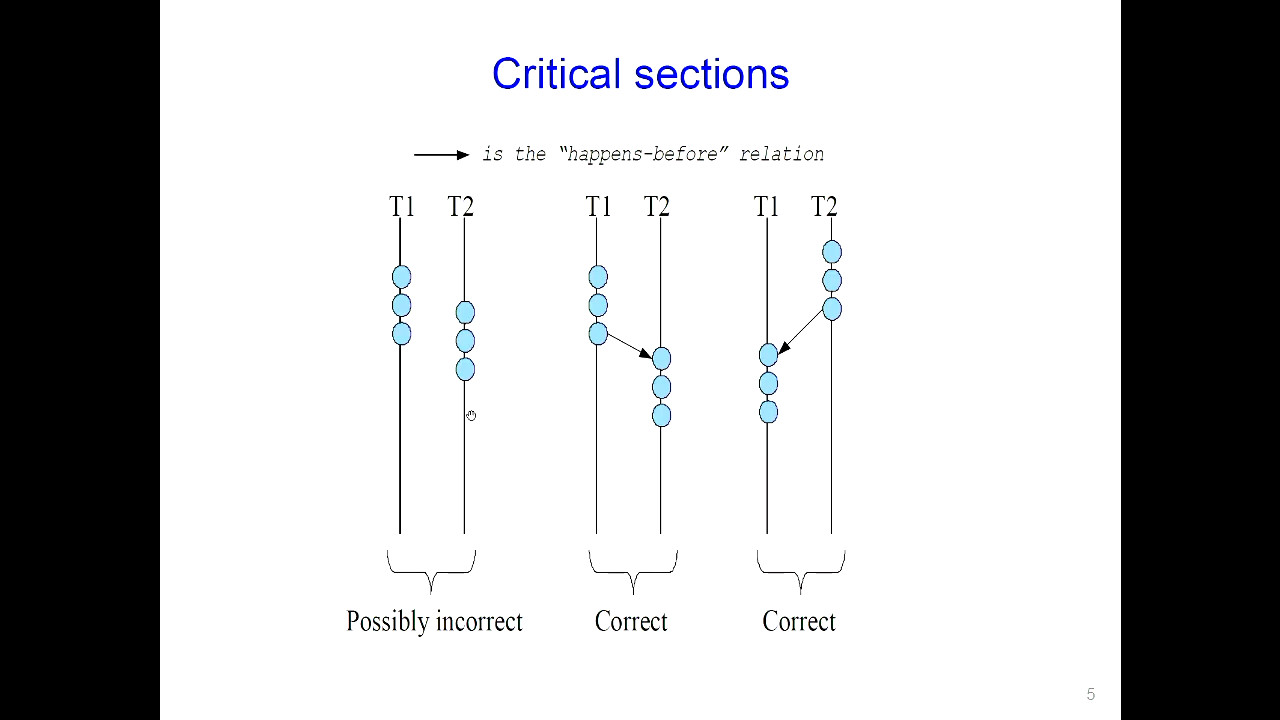
\includegraphics[height=270]{critical-sections.jpg}

\textbf{When do critical sections arise?}
\begin{itemize}
    \item One common pattern:
        \begin{itemize}
            \item read-modify-write of
            \item a shared value (variable)
            \item in code that can be executed by concurrent threads
        \end{itemize}
    \item Shared variable:
        \begin{itemize}
            \item Global and heap-allocated variables
            \item NOT local variables (which are on the stack)
        \end{itemize}
\end{itemize}

\textbf{Race conditions}
\begin{itemize}
    \item A program has a \emph{race condition} (data race) if the result of an
        execution depends on timing (i.e.\ it is non-deterministic)
    \item Typical symptoms
        \begin{itemize}
            \item I run it on the same data, and sometimes it prints 0 and sometimes 4
            \item I run it on the same data, and sometimes it prints 0 and sometimes crashes
        \end{itemize}
\end{itemize}

\textbf{Correct critical section requirements}
\begin{itemize}
    \item \emph{Mutual exclusion} \\
        At most one thread is in the critical section.
    \item \emph{Progress} \\
        If thread $T$ is outside the critical section,
        then $T$ cannot prevent thread $S$ from entering the critical section.
    \item \emph{Bounded waiting} (no \emph{starvation}) \\
        If thread $T$ is waiting on the critical section,
        then $T$ will eventually enter the critical section
        (assumes threads eventually leave critical sections).
    \item \emph{Performance} \\
        The overhead of entering and exiting the critical section is small with respect to
        the work being done within it.
\end{itemize}

\textbf{Mechanisms for building critical sections}
\begin{itemize}
    \item Spinlocks
        \begin{itemize}
            \item primitive, minimal semantics --- used to build others
        \end{itemize}
    \item Semaphores (and non-spinning locks)
        \begin{itemize}
            \item basic, easy to understand, somewhat hard to program with
        \end{itemize}
    \item Monitors
        \begin{itemize}
            \item higher level, requires language support, implicit operations
            \item easier to program with; Java ``\texttt{synchronised}'', for example
        \end{itemize}
    \item Messages
        \begin{itemize}
            \item Simple model of communication and synchronisation based on (atomic)
                transfer of data across a channel
            \item direct application to distributed systems
        \end{itemize}
\end{itemize}

\subsection{Locks}

\textbf{Locks}
\begin{itemize}
    \item A lock is a memory object with two operations:
        \begin{itemize}
            \item \texttt{acquire}: obtain the right to enter the critical section
            \item \texttt{release}: give up the right to be in the critical section
        \end{itemize}
    \item \texttt{acquire} \emph{prevents the progress of the thread until the lock
        can be acquired}.
    \item Note: terminology varies: acquire/release, lock/unlock
\end{itemize}

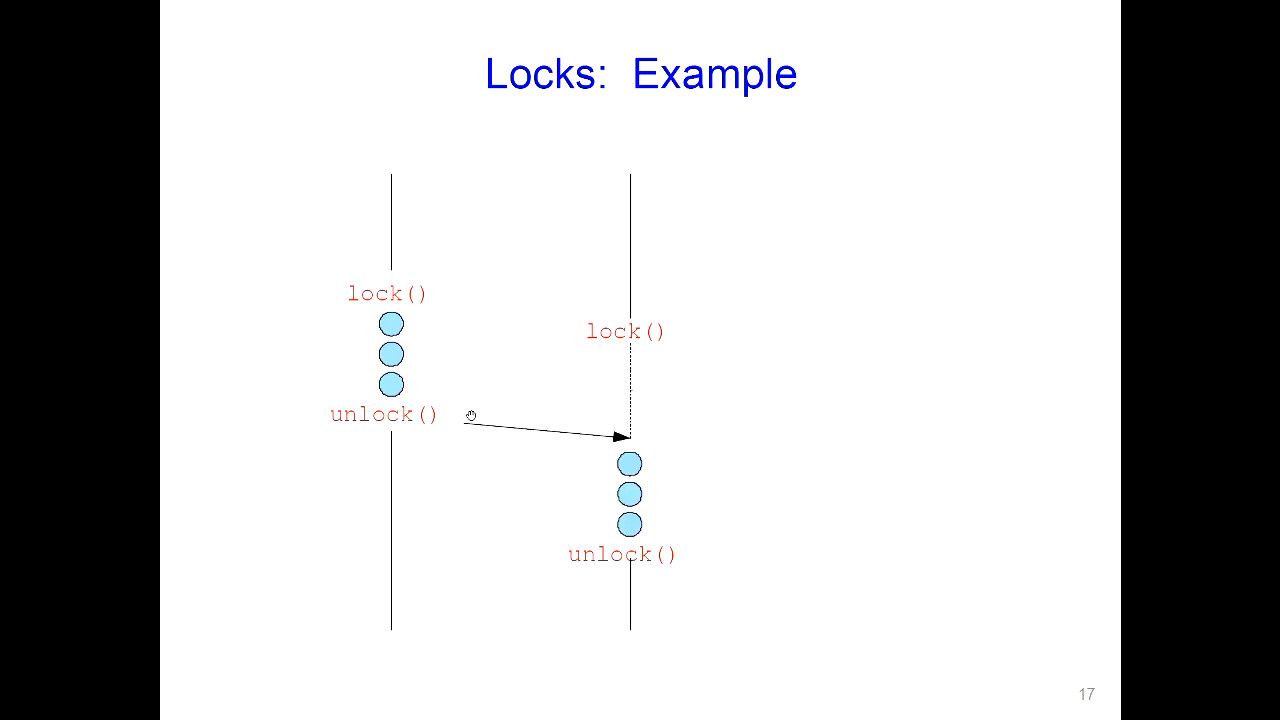
\includegraphics[height=270]{locks.jpg}

\textbf{Acquire/release}
\begin{itemize}
    \item Threads pair up calls to \texttt{acquire} and \texttt{release}
        \begin{itemize}
            \item between \texttt{acquire} and \texttt{release}, the thread \emph{holds}
                the lock
            \item \texttt{acquire} does not return until the caller ``owns'' (holds) the lock
                \begin{itemize}
                    \item at most one thread can hold a lock at a time
                \end{itemize}
        \end{itemize}
    \item What happens if the calls aren't paired
        \begin{itemize}
            \item I acquire, but neglect to release?
        \end{itemize}
    \item What happens if the two threads acquire different locks
        \begin{itemize}
            \item I think that access to a particular shared data structure is
                mediated by lock A, and you think it's mediated by lock B?\
        \end{itemize}
    \item What is the right granularity of locking?
\end{itemize}

\subsection{Spinlocks}

\textbf{Spinlocks}
\begin{itemize}
    \item How do we implement spinlocks?
        Here's one attempt:
        \begin{verbatim}
    struct lock_t {
        int held = 0;
    }
    void acquire(lock) {
        while (lock->held);
        lock->held = 1;
    }
    void release(lock) {
        lock->held = 0;
    }
        \end{verbatim}
    \item Race condition in acquire.
\end{itemize}

\textbf{Implementing spinlocks}
\begin{itemize}
    \item Problem is that implementation of spinlocks has critical sections, too!
        \begin{itemize}
            \item the acquire/release must be \emph{atomic}
            \item compiler can hoist code that is invariant
        \end{itemize}
    \item Need help from the hardware
        \begin{itemize}
            \item atomic instructions \\
                test-and-set, compare-and-swap, \dots
        \end{itemize}
\end{itemize}

\textbf{Spinlocks: Hardware Test-and-Set}
\begin{itemize}
    \item CPU provides the following as \emph{one atomic instruction}:
        \begin{verbatim}
    bool test_and_set(bool *flag) {
        bool old = *flag;
        *flag = True;
        return old;
    }
        \end{verbatim}
    \item This is a single \emph{atomic} instruction
\end{itemize}

\textbf{Implementing spinlocks using Test-and-Set}
\begin{itemize}
    \item So, to fix our broken spinlocks:
        \begin{verbatim}
    struct lock{
        int held = 0;
    }
    void acquire(lock) {
        while (test_and_set(&lock->held));
    }
    void release(lock) {
        lock->held = 0;
    }
    \end{verbatim}
\item \emph{mutual exclusion?} (at most one thread in the critical section)
\item \emph{progress?} (\texttt{T} outside cannot prevent \texttt{S} from entering)
\item \emph{bounded waiting?} (waiting \texttt{T} will eventually enter)
\item \emph{performance?} (low overhead (modulo the spinning part\dots))
\end{itemize}

\break{}

\section{Semaphores, Condition Variables, and Monitors}

\subsection{Semaphore}

\textbf{Semaphore}
\begin{itemize}
    \item More sophisticated synchronisation mechanism
    \item Semaphore \texttt{S} --- integer variable
    \item Can only be accessed via two atomic operations: \texttt{wait} and \texttt{signal}
        (originally called \texttt{P} and \texttt{V}).
    \item Definitions
        \begin{verbatim}
    wait(S) {
        while (S <= 0); // busy wait
        S--;
    }
    signal(S) {
        S++;
    }
        \end{verbatim}
    \item These are performed \emph{atomically}
\end{itemize}

\textbf{Semaphore Usage}
\begin{itemize}
    \item \emph{Counting semaphore}: integer value can range over an unrestricted domain
    \item \emph{Binary semaphore}: integer value can range only between 0 and 1
        (same as \emph{lock})
    \item Can solve various synchronisation problems
    \item Consider $\texttt{P}_1$ and $\texttt{P}_2$ that require $\texttt{S}_1$ to
        happen before $\texttt{S}_2$ \\
        Create a semaphore ``\texttt{synch}'' initialised to 0
        \begin{verbatim}
    P1:
        S_1;
        signal(synch);
    P2:
        wait(synch);
        S_2;
        \end{verbatim}
    \item Can implement a counting semaphore \texttt{S} as a binary semaphore.
\end{itemize}

\textbf{Implementation with no Busy waiting}

Each semaphore has an associated queue of threads
\begin{verbatim}
    wait(semaphore *S) {
        S->value--;
        if (S->value < 0) {
            add this thread to S->list;
            block();
        }
    }
    signal(semaphore *S) {
        S->value++;
        if (S->value <= 0) {
            remove a thread T from S->list;
            wakeup(T);
        }
    }
\end{verbatim}

\underline{Examples}

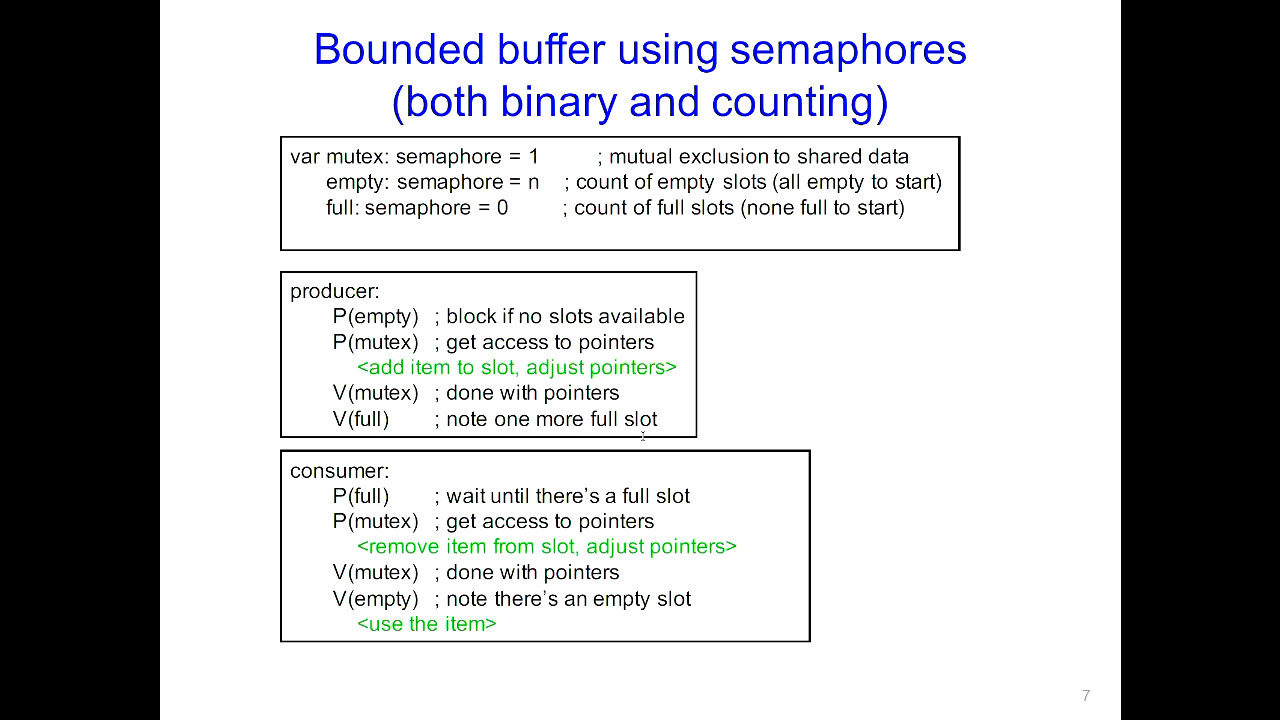
\includegraphics[height=270]{bounded-buffer-using-semaphores.jpg}

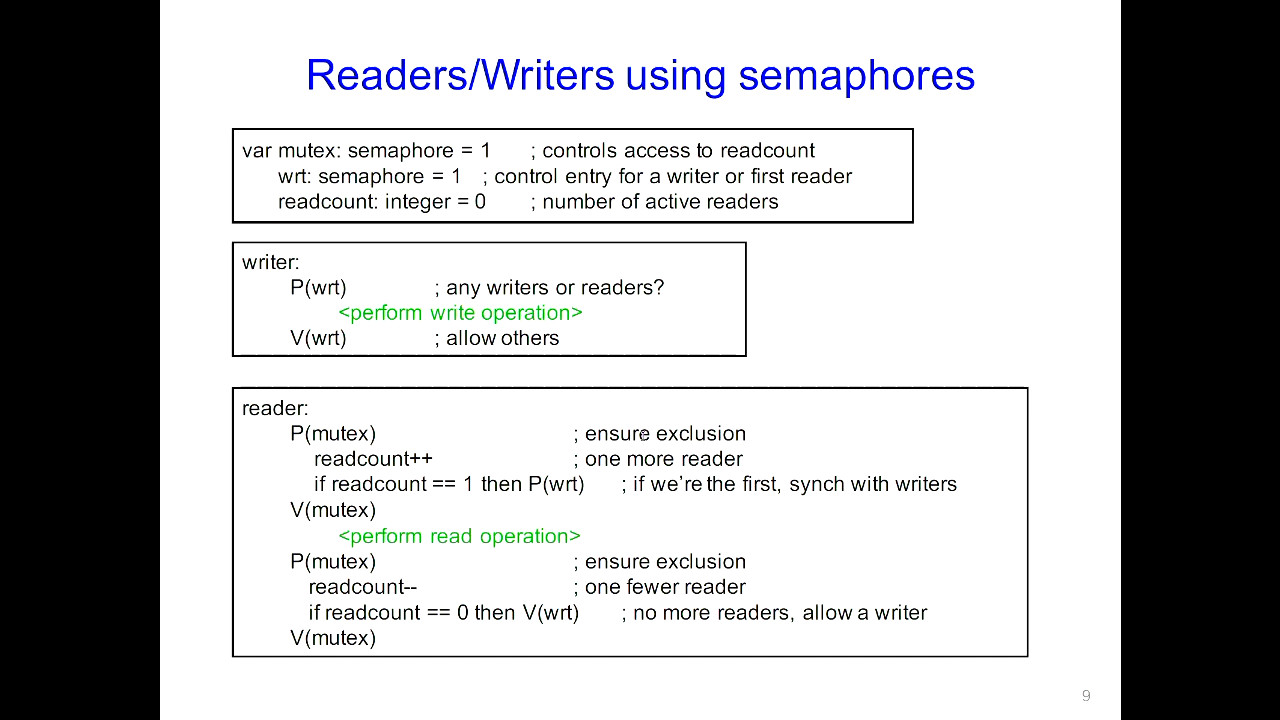
\includegraphics[height=270]{readers-writers-using-semaphores.jpg}

\textbf{Semaphores v.s.\ Spinlocks}
\begin{itemize}
    \item Threads that are blocked at the level of program logic
        (that is, by the semaphore \texttt{P} operation)
        are placed on queues, rather than busy-waiting.
    \item Busy-waiting may be used for the ``real'' mutual exclusion required to implement
        \texttt{P} and \texttt{V}
        \begin{itemize}
            \item but these are very short critical sections ---
                totally independent of program logic
            \item and they are not implemented by the application programmer.
        \end{itemize}
\end{itemize}

\textbf{Abstract implementation}
\begin{itemize}
    \item \texttt{P\,(sem)}
        \begin{itemize}
            \item acquire ``real'' mutual exclusion
                \begin{itemize}
                    \item if \texttt{sem} is ``available'' (> 0), decrement sum;
                        \emph{release ``real'' mutual exclusion};
                        let thread continue
                    \item otherwise,  place thread on associated queue;
                        \emph{release ``real'' mutual exclusion};
                        run some other thread.
                \end{itemize}
        \end{itemize}
    \item \texttt{V\,(sem)}
        \begin{itemize}
            \item \emph{acquire ``real'' mutual exclusion}
                \begin{itemize}
                    \item if threads are waiting on the associated queue,
                        unblock one (place it on the ready queue)
                    \item if no threads are on the queue, \texttt{sem} is incremented \\
                        the signal is ``remembered'' for the next time \texttt{P\,(sem)}
                        is called
                \end{itemize}
            \item release ``real'' mutual exclusion
            \item the ``\texttt{V}-ing'' thread continues execution.
        \end{itemize}
\end{itemize}

\textbf{Problems with semaphores, locks}
\begin{itemize}
    \item They can be used to solve any of the traditional synchronisation problems,
        but it's easy to make mistakes
        \begin{itemize}
            \item they are essentially shared global variables
                \begin{itemize}
                    \item can be accessed from anywhere (bad software engineering)
                \end{itemize}
            \item there is no connection between the synchronisation variable and the
                data being controlled by it
            \item no control over their use, no guarantee of proper usage
                \begin{itemize}
                    \item Semaphores: will here ever be a \texttt{V\,()}?
                    \item Locks: did you lock when necessary?
                        Unlock at the right time?
                        At all?
                \end{itemize}
        \end{itemize}
    \item Thus, they are prone to bugs
        \begin{itemize}
            \item We can reduce the chance of bugs by ``stylising'' the use of synchronisation
            \item Language help is useful for this.
        \end{itemize}
\end{itemize}

\subsection{Monitors}

\textbf{Monitors}
\begin{itemize}
    \item A \underline{programming language construct} supports controlled shared data access
        \begin{itemize}
            \item synchronisation code is added by the compiler.
        \end{itemize}
    \item A class in which every method automatically acquires a lock on entry,
        and releases it on exit --- it combines:
        \begin{itemize}
            \item \emph{shared data} structures (object);
            \item \emph{procedures} that operate on the shared data (object methods);
            \item \emph{synchronisation} between concurrent threads that invoke those
                procedures.
        \end{itemize}
    \item Data can only be accessed from within the monitor
        \begin{itemize}
            \item protects the data from unstructured access;
            \item prevents ambiguity about what the synchronisation variable protects.
        \end{itemize}
    \item Addresses the key usability issues that arise with semaphores.
\end{itemize}

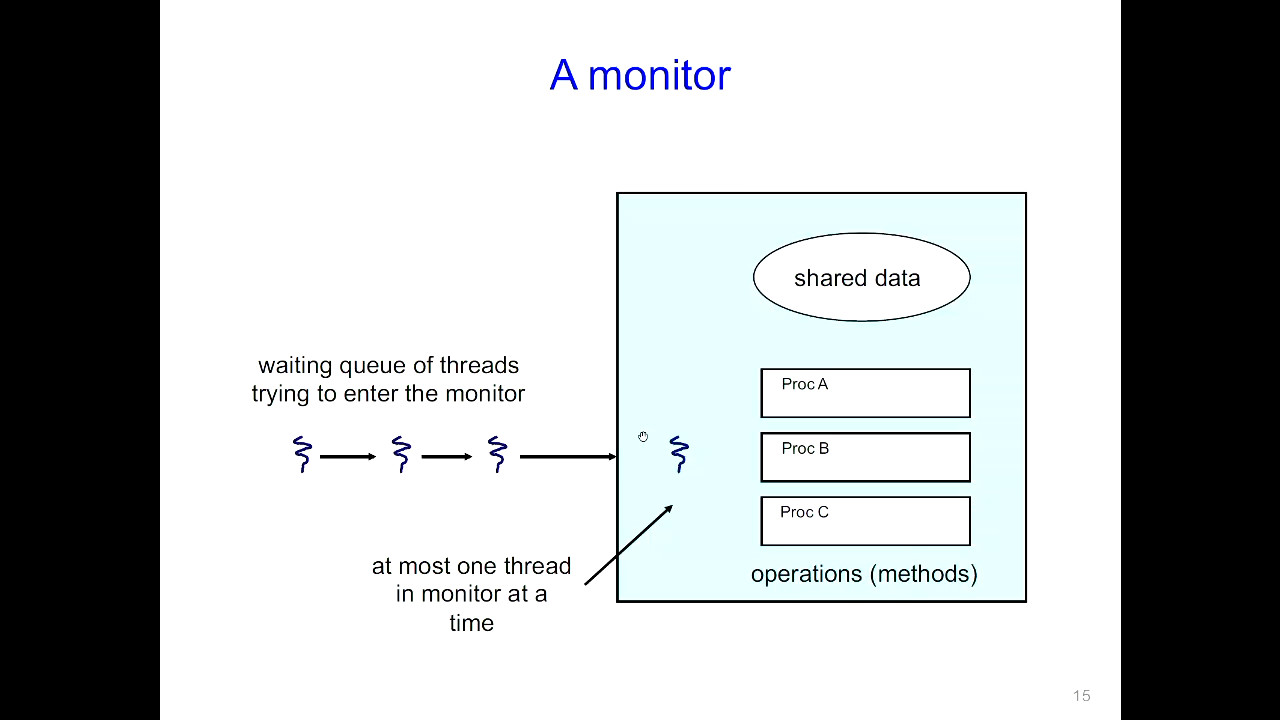
\includegraphics[height=270]{a-monitor.jpg}

\textbf{Monitor facilities}
\begin{itemize}
    \item ``Automatic'' mutual exclusion
        \begin{itemize}
            \item only one thread can be executing inside at any time
                \begin{itemize}
                    \item thus, synchronisation is implicitly associated with the monitor
                        --- it ``comes for free'';
                \end{itemize}
            \item if a second thread tries to execute a monitor procedure,
                it blocks until the first has left the monitor;
                \begin{itemize}
                    \item more restrictive than semaphores,
                    \item but easier to use (most of the time).
                \end{itemize}
        \end{itemize}
    \item But, there's a problem\dots \\
        Bounded buffer scenario.
\end{itemize}

\textbf{Bounded Buffer scenario}
\begin{itemize}
    \item Monitors require condition variables
    \item Operations on condition varibales
        \begin{itemize}
            \item \texttt{wait\,(c)}
                \begin{itemize}
                    \item release monitor lock, so somebody else can get in
                    \item wait for somebody else to signal condition
                    \item thus, condition variables have associated wait queues
                \end{itemize}
            \item \texttt{signal\,(c)}
                \begin{itemize}
                    \item wake up at most one waiting thread
                        \begin{itemize}
                            \item ``Hoare'' monitor: wakeup immediately, signaller steps
                                outside
                        \end{itemize}
                    \item if no waiting threads, signal is lost
                        \begin{itemize}
                            \item this is different from semaphores --- no history!
                        \end{itemize}
                \end{itemize}
            \item \texttt{broadcast\,(c)}
                \begin{itemize}
                    \item wake up all waiting threads.
                \end{itemize}
        \end{itemize}
\end{itemize}

\textbf{Bounded buffer using (Hoare) monitors}
\begin{verbatim}
    Monitor bounded_buffer {
        buffer resources[];
        condition not_full;
        condition not_empty;

        produce(resource x) {
            if (array "resources" is full, determined maybe by a count) {
                wait(not_full);
            }
            insert "x" in array "resources";
            signal(not_empty);
        }

        consume(resource *x) {
            if (array "resources" is empty, determined maybe by a count) {
                wait(not_empty);
            }
            *x = get resource from array "resources";
            signal(not_full);
        }
    }
\end{verbatim}

\textbf{Runtime system calls for (Hoare) monitors}
\begin{itemize}
    \item \texttt{EnterMonitor\,(m)} \{guarantee mutual exclusion\}
    \item \texttt{ExitMonitor\,(m)} \{hit the road, letting someone else run\}
    \item \texttt{Wait\,(c)} \{step out until condition satisfied\}
    \item \texttt{Signal\,(c)} \{if someone's waiting, step out and let them run\}
    \item \texttt{EnterMonitor} and \texttt{ExitMonitor} are inserted automatically by the
        compiler.
    \item This guarantees mutual exclusion for code inside of the monitor.
\end{itemize}

\textbf{Monitor Summary}
\begin{itemize}
    \item Language supports monitors
    \item Compiler understands them
        \begin{itemize}
            \item Compiler inserts calls to runtime routines for
                \begin{itemize}
                    \item monitor entry
                    \item monitor exit
                \end{itemize}
            \item Programmer inserts calls to runtime routines for
                \begin{itemize}
                    \item signal
                    \item wait
                \end{itemize}
            \item Language/object encapsulation ensures correctness
                \begin{itemize}
                    \item Sometimes!
                        With conditions, you \emph{still} need to think about synchronisation
                \end{itemize}
        \end{itemize}
    \item Runtime system implements these routines
        \begin{itemize}
            \item moves threads on and off queues
            \item \emph{ensures mutual exclusion!}
        \end{itemize}
\end{itemize}

\break{}

\section{Deadlock}

\textbf{Definition}
\begin{itemize}
    \item A thread is deadlocked when it's waiting for an event that can never occur
    \item Thread \texttt{A} is in critical section 1 \\
        waiting for access to critical section 2;
    \item Thread \texttt{B} is in critical section 2 \\ waiting for access to critical
        section 1
\end{itemize}

\textbf{Four conditions must exist for deadlock to be possible}
\begin{enumerate}
    \item Mutual exclusion
    \item Hold and wait
    \item No pre-emption
    \item Circular wait
\end{enumerate}

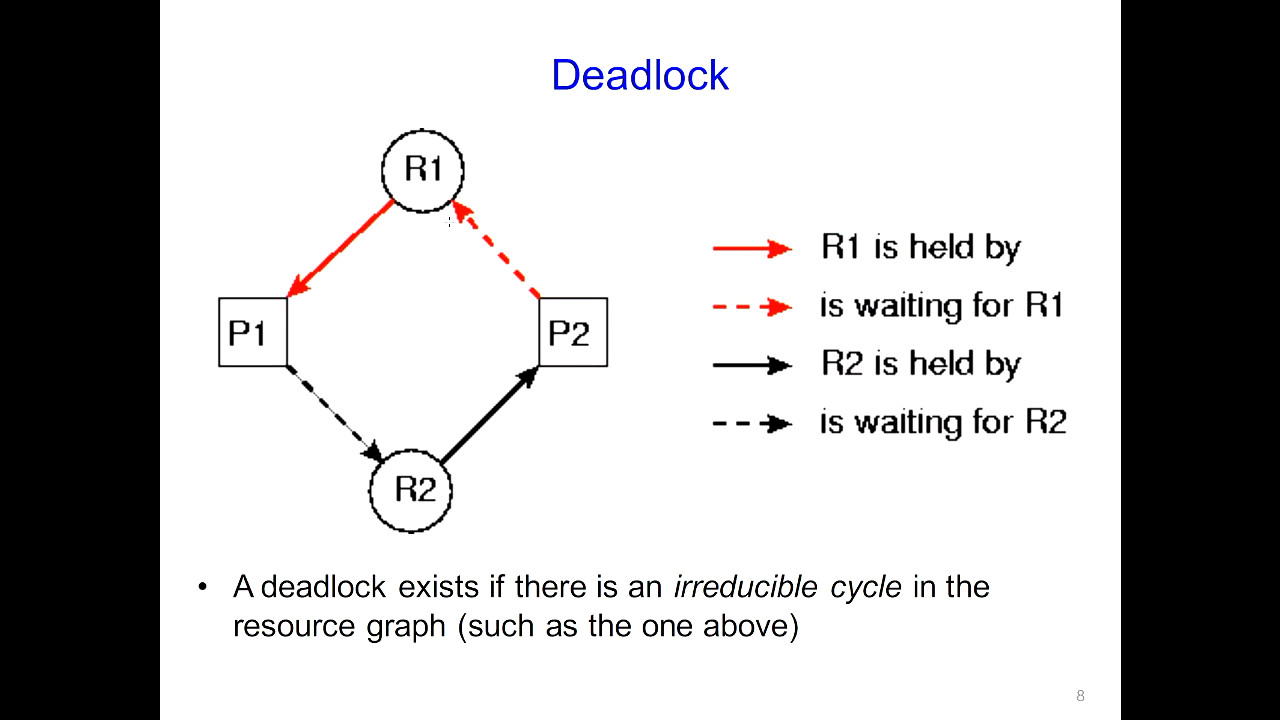
\includegraphics[height=270]{deadlock.jpg}

\subsection{Graph reduction}

\textbf{Graph reduction}
\begin{itemize}
    \item A graph can be \emph{reduced} by a thread if all of that thread's requests
        can be granted
        \begin{itemize}
            \item in this case, the thread eventually will terminate --- all resources are
                freed --- all arcs (allocations) to/from it in the graph are deleted.
        \end{itemize}
    \item Miscellaneous theorems (Holt, Havender):
        \begin{itemize}
            \item There are no deadlocked threads if and only if the graph is completely
                reducible.
            \item The order of reductions is irrelevant.
        \end{itemize}
\end{itemize}

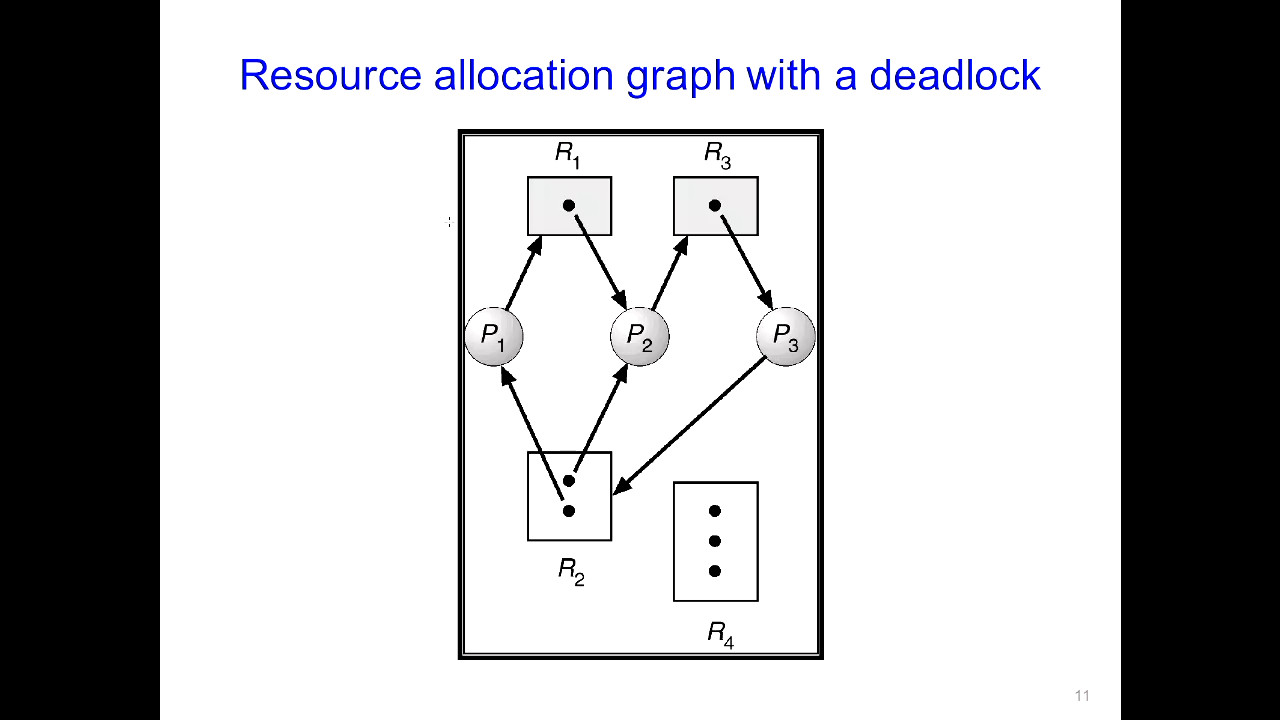
\includegraphics[height=270]{resource-allocation-graph-with-a-deadlock.jpg}

\textbf{Handling deadlock}
\begin{itemize}
    \item Eliminate one of the four required conditions
        \begin{itemize}
            \item Mutual exclusion
            \item Hold and Wait
            \item No pre-emption
            \item Circular wait
        \end{itemize}
    \item Broadly classified as:
        \begin{itemize}
            \item Prevention, or
            \item Avoidance, or
            \item Detection (and recovery)
        \end{itemize}
\end{itemize}

\textbf{Deadlock prevention} \\
Restrain the ways requests can be made
\begin{itemize}
    \item Mutual exclusion \\
        not required for sharable resources (e.g.\ read-only files);
        must hold for non-sharable resources.
    \item Hold and wait \\
        must guarantee that whenever a process requests a resources,
        it does not hold any other resources.
        \begin{itemize}
            \item Low resources utilisation; starvation is possible.
        \end{itemize}
    \item No (resource) Pre-emption
        \begin{itemize}
            \item If a process holding some resources requests another unavailable resource
                all resources currently held are released.
            \item Process will be restarted only when it can regain its old resources,
                as well as the new ones that it is requesting.
        \end{itemize}
    \item Circular wait
        \begin{itemize}
            \item impose a total ordering of all resource types, and require that each process
                requests resources in an increasing order of enumeration.
        \end{itemize}
\end{itemize}

\textbf{Avoidance} \\
Less severe restrictions on program behaviour.
\begin{itemize}
    \item Eliminating circular wait
        \begin{itemize}
            \item each thread states its maximum claim for every resource type;
            \item system runs the Banker's Algorithm at each allocation request \\
                Banker $\implies$ highly conservative
        \end{itemize}
\end{itemize}

\subsection{Banker's Algorithm}

\textbf{Banker's Algorithm example}
\begin{itemize}
    \item Background
        \begin{itemize}
            \item The set of controlled resources is known to the system.
            \item The number of units of each resource is known to the system.
            \item Each application must declare its maximum possible requirement of each
                resource type.
        \end{itemize}
    \item The, the system can do the following:
        \begin{itemize}
            \item When a request is made:
                \begin{itemize}
                    \item pretend you granted it;
                    \item pretend all other legal requests were made;
                    \item can the graph be reduced?
                        \begin{itemize}
                            \item If so: allocate the requested resource.
                            \item If not, block the thread until some thread releases
                                resources, and then try pretending again.
                        \end{itemize}
                \end{itemize}
        \end{itemize}
\end{itemize}

\textbf{Safe state}
\begin{itemize}
    \item When requesting an available resource decide if allocation leaves the system in a
        safe state
    \item We're in a \emph{safe state} if there exists a sequence $<P_1, P_2, \ldots, P_n>$
        of \emph{all} the processes in the systems
        \begin{itemize}
            \item such that for each $P_i$, the resources that $P_i$ can still request can be
                satisfied by currently available resources + resources held by all the $P_j$,
                with $j < i$.
        \end{itemize}
    \item That is:
        \begin{itemize}
            \item If $P_i$ resource needs are not immediately available, then $P_i$
                can wait until all $P_j$ have finished.
            \item When $P_j$ is finished, $P_i$ can obtain needed resources, execute, return
                allocated resources, and terminate.
            \item When $P_i$ terminates, $P_{i+1}$ can obtain its needed resources, and so on.
        \end{itemize}
\end{itemize}
Safe $\implies$ no deadlock; \quad deadlock $\implies$ unsafe

\textbf{Data Structures for the Banker's Algorithm}
Let \texttt{n} = number of processes, and \texttt{m} = number of resource types.
\begin{itemize}
    \item \texttt{Available}: Vector of length \texttt{m}.
        If \texttt{Available[j]} = \texttt{k}, there are \texttt{k} instances of resource type
        $\texttt{R}_\texttt{j}$ available.
    \item \texttt{Max} $\texttt{n} \times \texttt{m}$ matrix.
        If \texttt{Allocation[i,j]} = \texttt{k}, then $P_i$ is currently allocated
        \texttt{k} instances of $\texttt{R}_\texttt{j}$
    \item \texttt{Allocation}: $\texttt{n} \times \texttt{m}$ matrix.
        If \texttt{Need[i,j]} = \texttt{k}, then $\texttt{P}_\texttt{i}$ may need \texttt{k}
        more instances of $\texttt{R}_\texttt{j}$ to complete its task.
\end{itemize}
\[
    \texttt{Need[i,j]} = \texttt{Max[i,j]} - \texttt{Allocation[i,j]}
\]

\textbf{Safety Algorithm}
\begin{enumerate}
    \item Let \texttt{Work} and \texttt{Finish} be vectors of length \texttt{m} and \texttt{n},
        respectively.
        Initialise: \\
        \texttt{Work = Available} \\
        \texttt{Finish[i] = false for i = 0..n-1}
    \item Find an \texttt{i} such that both:
        \begin{enumerate}
            \item \texttt{Finish[i] == false}
            \item $\texttt{Need}_\texttt{i} \texttt{ <= Work}$
        \end{enumerate}
        If no such \texttt{i} exists, go to step 4
    \item \texttt{Work = Work + Allocation} \\
        \texttt{Finish[i] = true} \\
        go to step 2
    \item If \texttt{Finish[i] == true, for all i,}
        then the system is in a safe state.
\end{enumerate}

\textbf{Resource-Request Algorithm for Process $\texttt{P}_\texttt{i}$} \\
$\texttt{Request}_\texttt{i}$ = request vector for process $\texttt{P}_\texttt{i}$.
If $\texttt{Request}_\texttt{i}\texttt{[j] == k}$
then process $\texttt{P}_\texttt{i}$ wants \texttt{k} instances of resource type
$\texttt{R}_\texttt{j}$.
\begin{enumerate}
    \item If $\texttt{Request}_\texttt{i} \texttt{ <= Need}_\texttt{i}$ go to step 2.
        Otherwise raise error condition, since process has exceeded its maximum claim.
    \item If $\texttt{Request}_\texttt{i} \texttt{ <= Available}$, go to step 3.
        Otherwise $\texttt{P}_\texttt{i}$ must wait, since resources are not available.
    \item Pretend to allocate requested resources to $\texttt{P}_\texttt{i}$ by modifying
        the state as follows: \\
        $\texttt{Available = Available - Request}$ \\
        $\texttt{Allocation}_\texttt{i} \texttt{ =
        Allocation}_\texttt{i} \texttt{ + Request}_\texttt{i}$ \\
        $\texttt{Need}_\texttt{i} \texttt{ = Need}_\texttt{i} \texttt{ - Request}_\texttt{i}$
        \begin{enumerate}
            \item If safe, then resources allocated to $\texttt{P}_\texttt{i}$
            \item If unsafe, then $\texttt{P}_\texttt{i}$ must wait,
                and the old resource-allocation state is restored.
        \end{enumerate}
\end{enumerate}

\textbf{Deadlock Detection}
\begin{enumerate}
    \item Allow system to enter deadlock state
    \item Detection algorithm
    \item Recovery scheme
\end{enumerate}

\textbf{Single instance of each resource type}
\begin{itemize}
    \item Maintain a \emph{wait-for} graph
        \begin{itemize}
            \item Nodes are processes
            \item $\texttt{P}_\texttt{i} \to \texttt{P}_\texttt{j}$ if $\texttt{P}_\texttt{i}$
                is waiting for $\texttt{P}_\texttt{j}$
        \end{itemize}
    \item Periodically invoke an algorithm that searches for a cycle in the graph.
        \begin{itemize}
            \item If there is a cycle, there exists a deadlock.
        \end{itemize}
    \item An algorithm to detect a cycle in a graph
        \begin{itemize}
            \item has runtime complexity $\mathcal{O}(n^2)$ with $n$ being the number of
                vertices in the graph.
        \end{itemize}
\end{itemize}

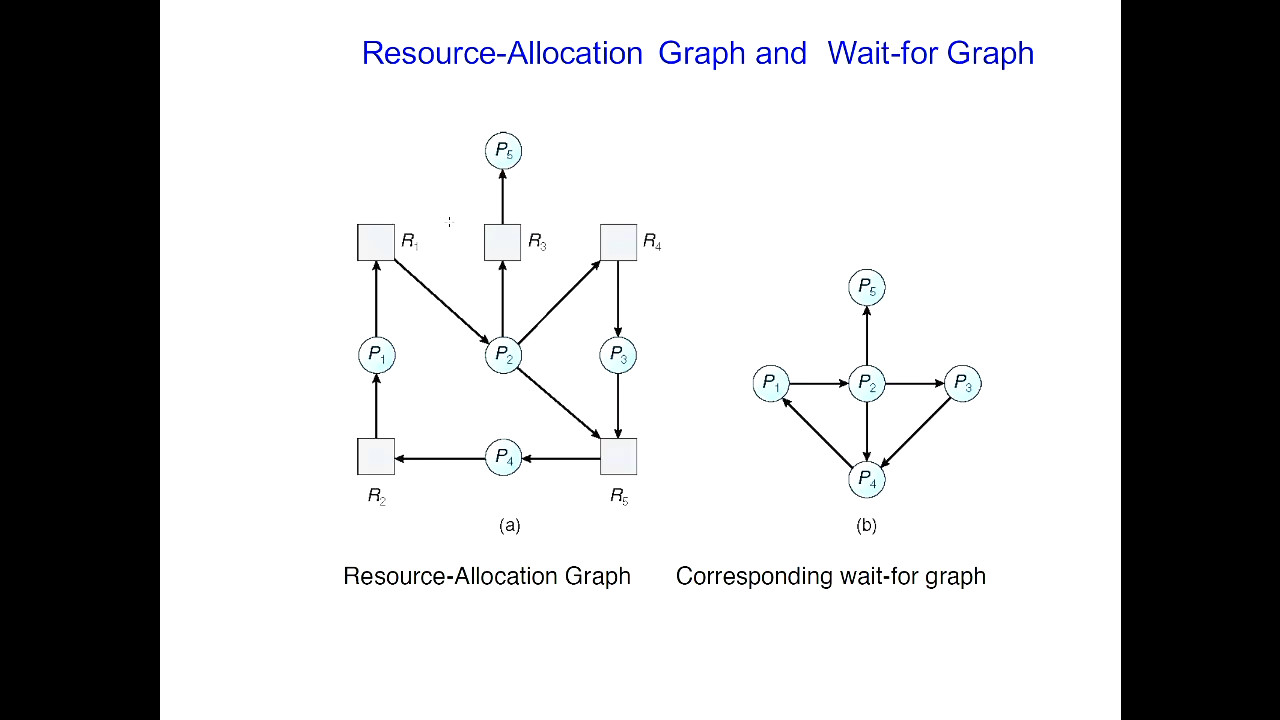
\includegraphics[height=270]{resource-allocation-graph-and-wait-for-graph.jpg}

\textbf{Detection-Algorithm usage}
\begin{itemize}
    \item When, and how often to invoke depends on:
        \begin{itemize}
            \item How often a deadlock is likely to occur?
            \item How many processes will need to be rolled back?
                \begin{itemize}
                    \item One for each disjoint cycle.
                \end{itemize}
        \end{itemize}
    \item If detection algorithm is invoked arbitrarily:
        \begin{itemize}
            \item there may be many cycles in the resource graph
            \item we would not be able to tell which deadlocked processes ``caused'' the
                deadlock.
        \end{itemize}
\end{itemize}

\textbf{Recovery from deadlock}
\begin{itemize}
    \item Process termination
        \begin{itemize}
            \item Abort all deadlocked processes
            \item Abort one process at a time until the deadlock cycle is eliminated
            \item In which order should we choose to abort?
        \end{itemize}
    \item Resource pre-emption
        \begin{itemize}
            \item \emph{Select a victim} --- minimise cost
            \item \emph{Rollback} --- return to some safe state,
                restart process for that state.
            \item \emph{Starvation} --- same process may always be picked as victim,
                include number of rollback in cost factor.
        \end{itemize}
\end{itemize}

\textbf{Summary}
\begin{itemize}
    \item Deadlock is bad!
    \item We can deal with it either statically (prevention)
        or dynamically (avoidance and/or detection)
    \item In practice, you'll encounter lock ordering, periodic deadlock detection/correction,
        and minefields.
\end{itemize}

\break{}

\section{Scheduling}

\textbf{Scheduling}
\begin{itemize}
    \item We have talked about \emph{context switching}
        \begin{itemize}
            \item an interrupt occurs (device completion, timer interrupt)
            \item a thread causes a trap or execution
            \item may need to choose a different thread/process to run
        \end{itemize}
    \item Glossed over which process or thread to run next
        \begin{itemize}
            \item ``some thread from the ready queue''
        \end{itemize}
    \item This decision is called \emph{scheduling}
        \begin{itemize}
            \item scheduling is a \emph{policy}
            \item context switching is a \emph{mechanism}
        \end{itemize}
\end{itemize}

\textbf{Classes of Schedulers}
\begin{itemize}
    \item Batch
        \begin{itemize}
            \item Throughput / utilisation oriented
            \item Example: audit inter-bank funds transfers each night, Pixar rendering,
                Hadoop/MapReduce jobs.
        \end{itemize}
    \item Interactive
        \begin{itemize}
            \item Response time oriented
        \end{itemize}
    \item Real time
        \begin{itemize}
            \item Deadline driven
            \item Example: embedded systems (cars, aeroplanes, etc.)
        \end{itemize}
    \item Parallel
        \begin{itemize}
            \item Speedup-driven
            \item Example: ``space-shared'' use of a 1000-processor machine for large
                simulations.
        \end{itemize}
\end{itemize}

\textbf{Multiple levels of scheduling decisions}
\begin{itemize}
    \item Long term
        \begin{itemize}
            \item Should a ``job'' be ``initiated'', or should it be held?
            \item Typical of batch systems.
        \end{itemize}
    \item Medium term
        \begin{itemize}
            \item Should a running program be temporarily marked as non-runnable
                (e.g.\ swapped out)?
        \end{itemize}
    \item Short term
        \begin{itemize}
            \item Which thread should be given to the CPU next?
                For how long?
            \item Which I/O operation should be sent to the disk next?
            \item On a multiprocessor:
                \begin{itemize}
                    \item Should we attempt to coordinate the running of threads from the same
                        address space in some way?
                    \item Should we worry about cache state (processor affinity)?
                \end{itemize}
        \end{itemize}
\end{itemize}

\subsection{Scheduling Goals}

\textbf{Scheduling Goals I:\@ Performance} \\
Many possible metrics / performance goals (which sometimes conflict)
\begin{itemize}
    \item maximise \emph{CPU utilisation}
    \item maximise \emph{throughput} (requests completed per second)
    \item minimise \emph{average response time} (average time from submission of request to
        completion of response)
    \item minimise \emph{average waiting time} (average time from submission of request to
        start of execution)
    \item minimise \emph{energy} (joules per instruction) subject to some constraint
        (e.g.\ frames per second)
\end{itemize}

\textbf{Scheduling Goals II:\@ Fairness}
\begin{itemize}
    \item No single, compelling definition of ``fair''
        \begin{itemize}
            \item How to measure fairness?
            \item Fair per-user? Per-process? Per-thread?
            \item What if one process is CPU bound, and one is I/O bound?
        \end{itemize}
    \item Sometimes the goal is to be unfair:
        \begin{itemize}
            \item Explicitly favour some particular class of requests (priority system),
                but\dots
            \item avoid starvation (be sure everyone gets at least some service).
        \end{itemize}
\end{itemize}

\textbf{When to assign?} \\
Pre-emptive v.s.\ non-pre-emptive schedulers
\begin{itemize}
    \item Non pre-emptive \\
        once you give somebody the green light, they've got it until they relinquish it
        \begin{itemize}
            \item an I/O operation
            \item allocation of memory in a system without swapping
        \end{itemize}
    \item Pre-emptive
        \begin{itemize}
            \item you can re-visit a decision
                \begin{itemize}
                    \item setting the timer allows you to pre-empt the CPU from a thread even
                        if it
                        doesn't relinquish it voluntarily.
                \end{itemize}
            \item Re-assignment always involves some overhead
                \begin{itemize}
                    \item Overhead doesn't contribute to the goal of any scheduler.
                \end{itemize}
        \end{itemize}
\end{itemize}
We'll assume ``work conserving'' policies
\begin{itemize}
    \item Never leave a resource idle when someone wants it
\end{itemize}

\subsection{Laws and properties}

\emph{The Utilisation Law}: $U = X \times S$
\begin{itemize}
    \item $U$ utilisation
    \item $X$ throughput (requests per second)
    \item $S$ average service time
    \item Utilisation is constant, independent of the schedule, so long as the workload
        can be processed
\end{itemize}

\emph{Little's Law}: $N = X \times R$
\begin{itemize}
    \item $N$ average number in system
    \item $X$ throughput
    \item $R$ average response time
    \item a better average response time implies fewer in system, and vice versa.
\end{itemize}

Response Time $R$ at a single server under FCFS scheduling:
\begin{itemize}
    \item $R = \frac{S}{1-U}$
    \item $N = \frac{U}{1-U}$
\end{itemize}

\subsection{Algorithms}

\textbf{Algorithm 1:\@ First-come first-served (FCFS)} \\
\begin{itemize}
    \item schedule in the order that they arrive
    \item ``real-world'' scheduling of people in (single) lines
    \item jobs treated equally, no starvation
    \item Drawbacks:
        \begin{itemize}
            \item Average response time can be poor: \emph{convoy effect}
            \item May lead to poor utilisation of other resources
                \begin{itemize}
                    \item if you send me on my way, I can go keep another resource busy
                    \item FCFS may result in poor overlap of CPU and I/O activity
                \end{itemize}
            \item The more copies of the resource there are to be scheduled
                \begin{itemize}
                    \item the less dramatic the impact of occasional very large jobs
                        (so long as there is a single waiting line)
                    \item e.g.\ multiple cores v.s.\@ single core
                \end{itemize}
        \end{itemize}
\end{itemize}

\textbf{Algorithm 2:\@ Shortest-job-first (SJF)}
\begin{itemize}
    \item Associate with each process the length of its next CPU burst
        \begin{itemize}
            \item use these lengths to schedule the process with the shortest time
        \end{itemize}
    \item SJF is optimal --- gives minimum average waiting time for a given set of processes
        \begin{itemize}
            \item the difficulty is knowing the length of the next CPU request
            \item could ask the user.
        \end{itemize}
    \item Determining the length of next CPU burst
        \begin{itemize}
            \item Can only estimate the length --- should be similar to the previous one
                \begin{itemize}
                    \item then pick process with shortest predicted next CPU burst.
                \end{itemize}
            \item Can be done by  using the length of previous CPU bursts, using exponential
                averaging
                \begin{enumerate}
                    \item $t_n$ actual length of $n$th CPU burst
                    \item $\tau_{n+1}$ predicted value for the next CPU burst
                    \item $\alpha, 0 \leq \alpha \leq 1$
                    \item Define: $\tau_{n+1} = \alpha t_n + (1-\alpha)\tau_n$
                \end{enumerate}
            \item Commonly, set $\alpha = 0.5$
            \item Pre-emptive version called \emph{shortest-remaining-time-first}
        \end{itemize}
\end{itemize}

\textbf{Algorithm 3:\@ Round Robin (RR)}
\begin{itemize}
    \item Each process gets a small unit of CPU time (\emph{time quantum} $q$),
        usually 10--100 milliseconds.
        \begin{itemize}
            \item After this time has elapsed, the process is pre-empted and added to the
                end of the ready queue.
        \end{itemize}
    \item If there are $n$ processes in the ready queue and the time quantum is $q$,
        \begin{itemize}
            \item then each process gets $\frac{1}{n}$ of the CPU time in chunks of at most
                $q$ time units at once.
            \item No process waits more than $(n-1)q$ time units.
        \end{itemize}
    \item Timer interrupts every quantum to schedule next process
    \item Performance
        \begin{itemize}
            \item $q$ large $\implies$ FIFO
            \item $q$ small $\implies q$ must be large with respect to context switch,
                otherwise overhead is too high.
        \end{itemize}
    \item Drawbacks:
        \begin{itemize}
            \item What if all jobs are exactly the same length?
            \item What do you set the quantum to be?
                \begin{itemize}
                    \item no value is ``correct''
                    \item if small, then context switch often, incurring high overhead
                    \item if large, then the response time degrades.
                \end{itemize}
            \item Treats all jobs equally
        \end{itemize}
\end{itemize}

\textbf{Algorithm 4:\@ Priority Scheduling}
\begin{itemize}
    \item A priority number (integer) is associated with each process
    \item The CPU is allocated to the process with the highest priority
    \item SJF is priority scheduling where priority is the inverse of predicted next CPU
        burst time.
    \item Problem: \emph{starvation} --- low priority processes may never execute.
    \item Solution: \emph{ageing} --- as time progresses, increase the priority of the process.
\end{itemize}

\textbf{Multi-level Feedback Queues (MLFQ)}
\begin{itemize}
    \item It's been observed that workloads tend to have increasing residual life ---
        ``if you don't finish quickly, you're probably a lifer''
    \item This is exploited in practice by using a policy that discriminates against the old.
    \item MLFQ:\@
        \begin{itemize}
            \item there is a hierarchy of queues
            \item there is a priority ordering among the queues
            \item new requests enter the highest priority queue
            \item each queue is scheduling RR
            \item requests move between queues based on execution history.
        \end{itemize}
\end{itemize}

\textbf{Unix scheduling}
\begin{itemize}
    \item Canonical scheduler is pretty much MLFQ
        \begin{itemize}
            \item 3--4 classes spanning $\sim170$ priority levels
                \begin{itemize}
                    \item time-sharing: lowest 60 priorities
                    \item system: middle 40 priorities
                    \item real-time: highest 60 priorities
                \end{itemize}
            \item priority scheduling across queues, RR within
                \begin{itemize}
                    \item process with highest priority always run first
                    \item processes with same priority scheduled RR
                \end{itemize}
            \item processes dynamically change priority
                \begin{itemize}
                    \item increases over time if process blocks before end of quantum
                    \item decreases if process uses entire quantum
                \end{itemize}
        \end{itemize}
    \item Goals:
        \begin{itemize}
            \item reward interactive behaviour over CPU hogs
                \begin{itemize}
                    \item interactive jobs typically have short bursts of CPU
                \end{itemize}
        \end{itemize}
\end{itemize}

\subsection{Summary}
\begin{itemize}
    \item Scheduling takes place at many levels
    \item It can make a huge difference in performance
        \begin{itemize}
            \item this difference increases with the variability in service requirements
        \end{itemize}
    \item Multiple goals, sometimes conflicting
    \item There are many ``pure'' algorithms, most with some drawbacks in practice ---
        FCFS, SJF, RR, Priority
    \item Real system use hybrids that exploit observed program behaviour
    \item Scheduling is important
\end{itemize}

\break{}

\section{Memory Management}

\subsection{Background}

\textbf{Goals and Tools of memory management}
\begin{itemize}
    \item Allocate memory resources among competing processes
        \begin{itemize}
            \item maximising memory utilisation and system throughput
        \end{itemize}
    \item Provide isolation between processes
        \begin{itemize}
            \item Addressability and protection: orthogonal
        \end{itemize}
    \item Convenient abstraction for programming
        \begin{itemize}
            \item and compilers, etc.
        \end{itemize}
    \item Tools
        \begin{itemize}
            \item Base and limit registers
            \item Swapping
            \item Segmentation
            \item Paging, page tables, and TLB
            \item Virtual memory
        \end{itemize}
\end{itemize}

\textbf{Background}
\begin{itemize}
    \item Program must be brought (from disk) into memory and placed within a process for it
        to be run.
    \item Main memory and registers are only storage CPU can access directly.
    \item Memory unit only sees a stream of address + read requests, or addresses + data
        and write requests
    \item Register access in one CPU clock (or less)
    \item Main memory can take many cycles, causing a \emph{stall}
    \item \emph{Cache} sits between main memory and CPU registers.
    \item Protection of memory required to ensure correct operation.
\end{itemize}

\textbf{Base and Limit Registers}
\begin{itemize}
    \item A pair of \emph{base} and \emph{limit} registers define the logical address
        space.
    \item CPU must check every memory access generated in user mode to be sure it is
        between base and limit for that user.
\end{itemize}

\subsection{Logical/Virtual address space v.s.\ Physical address space}

\textbf{Virtual address for multiprogramming}
\begin{itemize}
    \item To make it easier to manage memory of multiple processes,
        make processes \emph{use logical or virtual address}
        \begin{itemize}
            \item Logical/virtual addresses are independent of location in physical
                memory data lives
                \begin{itemize}
                    \item OS determines location in physical memory.
                \end{itemize}
        \end{itemize}
    \item Instructions issued by CPU reference logical/virtual addresses
        \begin{itemize}
            \item e.g.\ pointers, arguments to load/store instructions, PC, etc.
        \end{itemize}
    \item Logical/virtual addresses are translated by hardware into physical addresses
        (with some setup from OS).
\end{itemize}

\textbf{Logical/Virtual Address Space}
\begin{itemize}
    \item The set of logical/virtual addresses a process can reference is its
        \emph{address space}
        \begin{itemize}
            \item many different possible mechanisms for translating logical/virtual
                addresses to physical addresses.
        \end{itemize}
    \item Program issues addresses in a logical/virtual address space
        \begin{itemize}
            \item must be \emph{translated} to physical address space;
            \item think of the program as having a contiguous logical/virtual address
                space that starts at 0;
                and a contiguous physical address space that starts somewhere else.
        \end{itemize}
    \item \emph{Logical/virtual address space} is the set of all logical addresses
        generated by a program.
    \item \emph{Physical address space} is the set of all physical addresses generated
        by a program.
\end{itemize}

\textbf{Memory-Management Unit (MMU)}
\begin{itemize}
    \item Hardware device
        \begin{itemize}
            \item at runtime maps virtual to physical addresses
        \end{itemize}
    \item Many methods possible
    \item Simple scheme: value in relocation register is added to every address generated by
        a user process at the time it is sent to memory.
        \begin{itemize}
            \item Base register now called \emph{relocation register}
        \end{itemize}
    \item The user program deals with \emph{logical} addresses --- it never sees the
        \emph{real} physical addresses.
        \begin{itemize}
            \item Execution-time binding occurs when reference is made to location in
                memory.
            \item Logical address bound to physical addresses.
        \end{itemize}
\end{itemize}

\subsection{Swapping}

\textbf{Swapping}
\begin{itemize}
    \item What if not enough memory to hold all processes?
    \item A process can be \emph{swapped} temporarily
        \begin{itemize}
            \item out of memory to a backing store,
            \item brought back into memory for continued execution
            \item total physical memory space of processes can exceed physical memory.
        \end{itemize}
    \item \emph{Backing store} --- fast disk
        \begin{itemize}
            \item large enough to accommodate copies of all memory images for all users;
            \item must provide direct access to these memory images.
        \end{itemize}
    \item \emph{Roll out, roll in} --- swapping variant
        \begin{itemize}
            \item used for priority-based scheduling algorithms;
            \item lower-priority process is swapped out so higher-priority processes
                can be loaded and executed.
        \end{itemize}
    \item Major part of swap time is transfer time
        \begin{itemize}
            \item total transfer time is directly proportional to the amount of memory swapped.
        \end{itemize}
    \item System maintains a \emph{ready queue}
        \begin{itemize}
            \item ready-to-run processes which have memory images on disk.
        \end{itemize}
\end{itemize}

\textbf{Context Switch Time including Swapping}
\begin{itemize}
    \item If next processes to be put on CPU is not in memory
        \begin{itemize}
            \item need to swap out a process and swap in target process.
        \end{itemize}
    \item Context switch time can then be very high
    \item Can reduce cost
        \begin{itemize}
            \item reduce size of --- by knowing how much memory really being used;
            \item inform OS of memory use via \texttt{request\_memory\,()} and
                \texttt{release\_memory\,()}.
        \end{itemize}
    \item Other constraints as well on swapping
        \begin{itemize}
            \item Pending I/O --- can't swap out as I/O would occur to wrong process.
        \end{itemize}
    \item Or always transfer I/O to kernel space, then I/O device
        \begin{itemize}
            \item known as \emph{double buffering}, adds overhead.
        \end{itemize}
    \item Standard swapping not used in modern operating systems
        \begin{itemize}
            \item But modified version common
                \begin{itemize}
                    \item Swap only when free memory extremely low.
                \end{itemize}
        \end{itemize}
\end{itemize}

\subsection{Contiguous Memory Allocation}

\textbf{Contiguous Allocation}
\begin{itemize}
    \item Main memory must support both OS and user processes
    \item Limited resource, must allocate efficiently
    \item Contiguous allocation is one early method
    \item Main memory usually into two \emph{partitions}:
        \begin{itemize}
            \item Resident OS, usually held in low memory with interrupt vector;
            \item User processes then held in high memory;
            \item Each process contained in single contiguous section of memory.
        \end{itemize}
    \item Relocation registers
        \begin{itemize}
            \item used to protect user processes from each other, and from changing
                OS code and data;
            \item base register contains value of smallest physical address;
            \item limit register contains range of logical addresses --- each logical
                address must be less than the limit register.
        \end{itemize}
    \item MMU maps logical address \emph{dynamically}
        \begin{itemize}
            \item can then allow actions such as kernel code being \emph{transient}
                and kernel changing size.
        \end{itemize}
\end{itemize}

\textbf{Multiple-partition allocation}
\begin{itemize}
    \item Degree of multiprogramming limited by number of partitions
    \item 2 approaches
        \begin{itemize}
            \item Fixed partition
            \item Variable partition
        \end{itemize}
\end{itemize}

\textbf{Old technique 1:\ Fixed partitions}
\begin{itemize}
    \item Physical memory is broken up into fixed partitions
        \begin{itemize}
            \item partitions may have different sizes, but partitioning never changes
            \item hardware requirement: \emph{base/relocation register},
                \emph{limit register}
                \begin{itemize}
                    \item physical address = logical address + base register
                    \item base register loaded by OS when it switches to a process
                \end{itemize}
        \end{itemize}
    \item Advantages:
        \begin{itemize}
            \item Simple
        \end{itemize}
    \item Problems
        \begin{itemize}
            \item \emph{internal fragmentation}: the available partition is larger than what
                was requested.
        \end{itemize}
\end{itemize}

\textbf{Old technique 2:\ Variable partitions}
\begin{itemize}
    \item Obvious next step: physical memory is broken up into partitions dynamically ---
        partitions are tailored to programs
        \begin{itemize}
            \item hardware requirements: \emph{base register}, \emph{limit register}
            \item physical address = logical address + base register
        \end{itemize}
    \item Advantages
        \begin{itemize}
            \item no internal fragmentation
                \begin{itemize}
                    \item simply allocate partition size to be just big enough for process
                        (assuming we know what that is!)
                \end{itemize}
        \end{itemize}
    \item Problems
        \begin{itemize}
            \item \emph{external fragmentation}
                \begin{itemize}
                    \item as we load and unload jobs, holes are left scattered throughout
                        physical memory.
                \end{itemize}
        \end{itemize}
\end{itemize}

\textbf{Multiple-partition allocation}
\begin{itemize}
    \item \emph{Variable-partition} sizes for efficiency (sized to a given process' needs).
    \item \emph{Hole} --- block of available memory; holes of various sizes are scattered
        throughout memory.
    \item When a process arrives, allocated memory from a hole large enough to accommodate
        it.
    \item Process exiting frees its partition, adjacent free partitions combined.
    \item OS maintains information about:
        \begin{enumerate}
            \item allocated partitions,
            \item free partitions (hole)
        \end{enumerate}
\end{itemize}

\textbf{Dynamic Storage-Allocation Problem}
\begin{itemize}
    \item \emph{First-fit}: Allocate the \emph{first} hole that is big enough
    \item \emph{Best-fit}: Allocate the \emph{smallest} hole that is big enough;
        must search entire list, unless ordered by size
        \begin{itemize}
            \item produces the smallest leftover hole.
        \end{itemize}
    \item \emph{Worst-fit}: Allocates the \emph{largest} hole; must also search the entire list
        \begin{itemize}
            \item produces the largest leftover hole
        \end{itemize}
\end{itemize}
First-fit and best-fit better than worst-fit in terms of speed and storage utilisation.

\textbf{Fragmentation}
\begin{itemize}
    \item \emph{External fragmentation}: total memory space exists to satisfy a request,
        but it is not contiguous;
    \item \emph{Internal fragmentation}: allocated memory may be slightly larger than
        requested memory;
    \item First fit analysis reveals that given $N$ blocks allocated, $0.5N$ blocks lost
        to fragmentation
    \item $\frac{1}{3}$ may be unusable $\implies$ \emph{50 percent rule}.
\end{itemize}

\textbf{Dealing with fragmentation}
\begin{itemize}
    \item Compact memory by copying
        \begin{itemize}
            \item Swap a program out
            \item Reload it, adjacent to another
            \item Adjust its base register
            \item Compaction is possible \emph{only} if relocation is dynamic
            \item I/O problem:
                \begin{itemize}
                    \item Latch job in memory while it is involved in I/O
                    \item Do I/O only into OS buffers
                \end{itemize}
        \end{itemize}
\end{itemize}

\subsection{Segmentation}

\textbf{Segmentation}
\begin{itemize}
    \item Dealing with fragmentation
        \begin{itemize}
            \item Why not remove the need for continuous addresses?
        \end{itemize}
    \item Segmentation
        \begin{itemize}
            \item partition an address space into \emph{logical} units
                \begin{itemize}
                    \item stack, code, heap, subroutines
                \end{itemize}
            \item a virtual address is \texttt{<segment\#, offset>}
        \end{itemize}
    \item Facilitates sharing and reuse
        \begin{itemize}
            \item a segment is a natural unit of sharing --- a subroutine or function
        \end{itemize}
    \item A natural extension of variable-sized partitions
        \begin{itemize}
            \item variable-sized partition = 1 segment per process
            \item segmentation = many segments per process.
        \end{itemize}
\end{itemize}

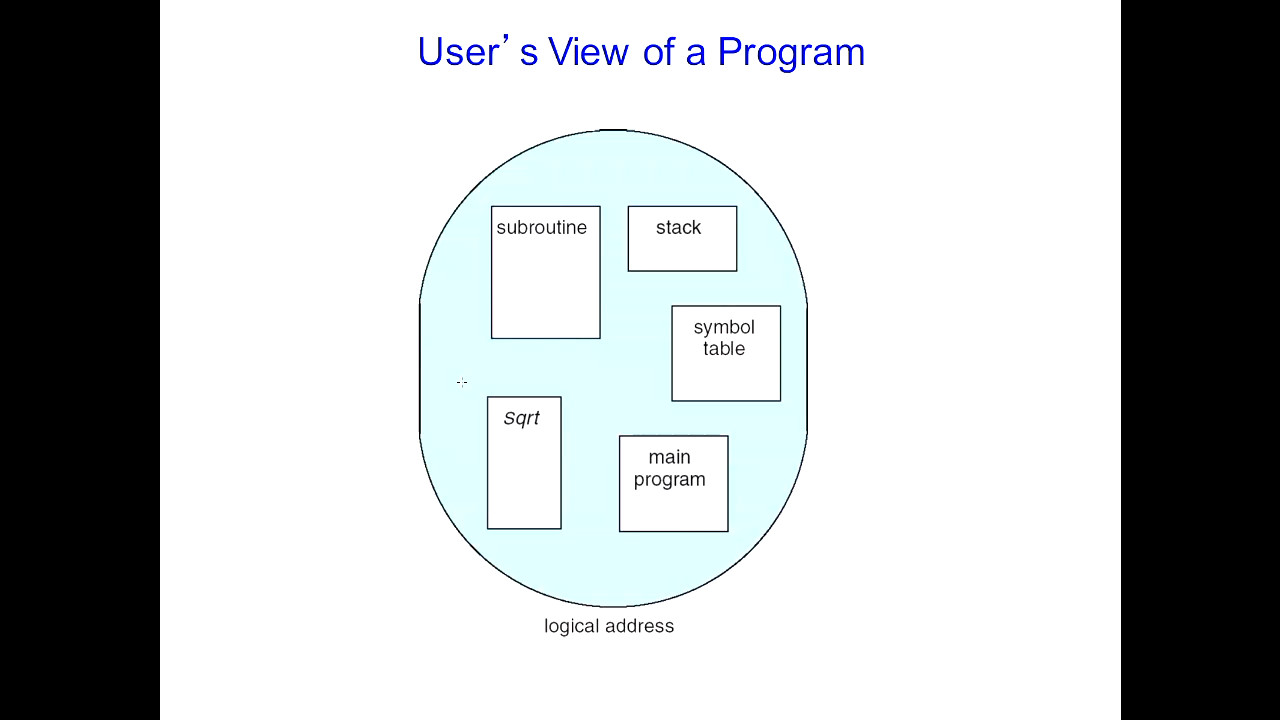
\includegraphics[height=270]{users-view-of-a-program.jpg}

\textbf{Hardware support}
\begin{itemize}
    \item Segment table
        \begin{itemize}
            \item multiple base/limit pairs, \emph{one per segment}
            \item segments named by segment\#, used as index into table
                \begin{itemize}
                    \item a virtual address is \texttt{<segment\#, offset>}
                \end{itemize}
            \item offset of virtual address added to base address of segment to yield
                physical address
        \end{itemize}
\end{itemize}

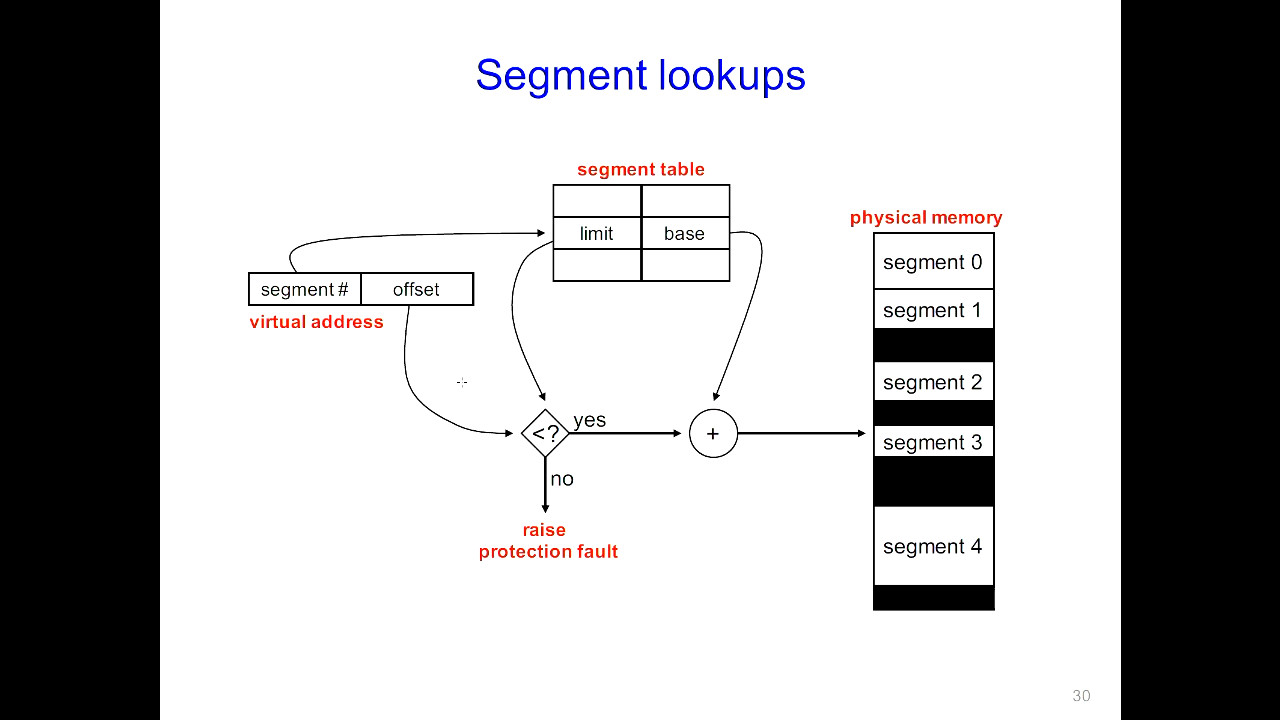
\includegraphics[height=270]{segment-lookups.jpg}

\textbf{Pros and Cons}
\begin{itemize}
    \item Logical and it facilitates sharing and reuse
    \item Allows non-contiguous physical addresses
        \begin{itemize}
            \item Helps exploit varying sized holes
        \end{itemize}
    \item But it has the complexity of a variable partition system
        \begin{itemize}
            \item except that linking is simpler, and the ``chunks'' that must be allocated
                are smaller than a ``typical'' linear address space.
        \end{itemize}
    \item Segmentation rarely used alone
        \begin{itemize}
            \item Paging is the basis for modern memory management
        \end{itemize}
\end{itemize}

\subsection{Summary}

\begin{itemize}
    \item Logical/Virtual Address Space v.s. Physical Address Space
    \item Swapping
    \item Contiguous memory allocation
    \item Fragmentation
    \item Segmentation
    \item Paging
        \begin{itemize}
            \item A better solution
        \end{itemize}
\end{itemize}

\break{}

\section{Paging}

\subsection{Paging}

\textbf{Address translation scheme}
\begin{itemize}
    \item Address generated by CPU is divided into:
        \begin{itemize}
            \item \emph{Page number} ($p$) --- used as an index into a \emph{page table}
                which contains base address of each page in physical memory
            \item \emph{Page offset} ($d$) --- combined with base address to define the
                physical memory address that is sent to the memory unit
        \end{itemize}
\end{itemize}

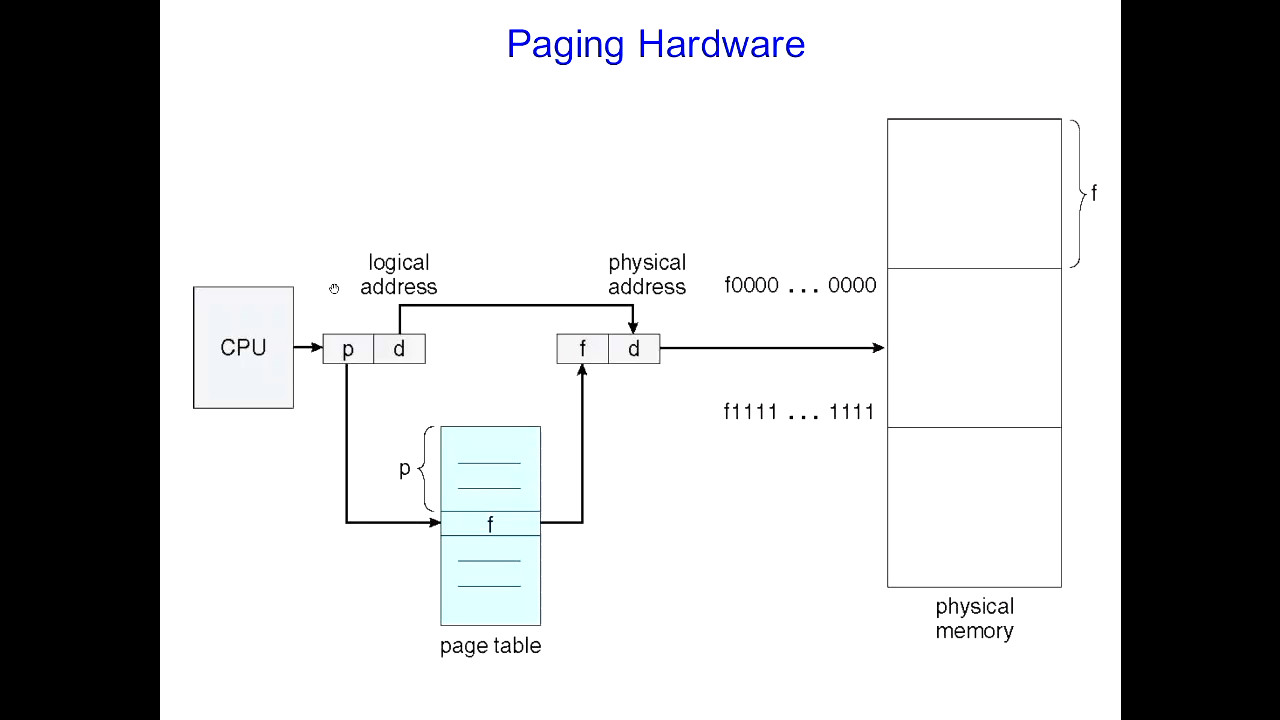
\includegraphics[height=270]{paging-hardware.jpg}
\subsection{Page Tables}

\textbf{Implementation of Page Table}
\begin{itemize}
    \item Page table is kept in main memory
    \item Page-table base register (PTBR) points to the page table
    \item Page-table length register (PTLR) indicates the size of the page table
    \item In this scheme, every data/instruction access requires two memory access
        \begin{itemize}
            \item one for the page table, and one for the data/instruction
        \end{itemize}
    \item The two memory access problem can be solved
        \begin{itemize}
            \item by the use of a special fast-lookup hardware cache
            \item called \emph{associative memory} or \emph{translation look-aside buffers}
                (TLBs)
        \end{itemize}
    \item Some TLBs store \emph{address-space identifiers} (ASIDs) in each TLB entry
        \begin{itemize}
            \item uniquely identifies each process;
            \item provides address-space protection for that process;
            \item otherwise need to flush at every context switch.
        \end{itemize}
    \item TLBs typically small (64--1,024 entries)
    \item On a TLB miss, value is loaded into the TLB for faster access next time.
        \begin{itemize}
            \item Replacement policies must be considered.
            \item Some entries can be \emph{wired down} for permanent fast access.
        \end{itemize}
\end{itemize}

\subsection{TLB}

\textbf{Associative Memory}
\begin{itemize}
    \item Associative memory --- parallel search
    \item Address translation ($p$, $d$)
        \begin{itemize}
            \item if $p$ is in associative register, get frame\# out;
            \item otherwise get frame\# from page table in memory.
        \end{itemize}
\end{itemize}

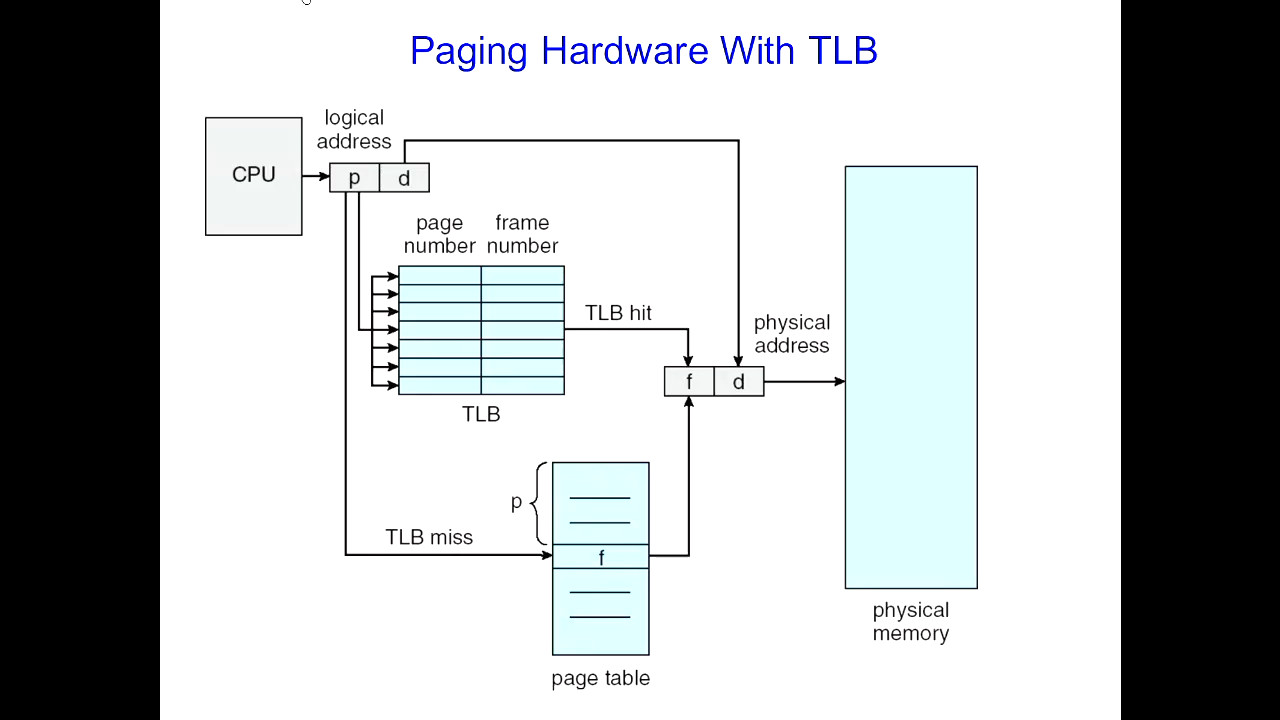
\includegraphics[height=270]{paging-hardware-with-tlb.jpg}

\textbf{Effective Access Time}
\begin{itemize}
    \item Associative lookup
        \begin{itemize}
            \item Extremely fast
        \end{itemize}
    \item Hit ratio = $\alpha$
        \begin{itemize}
            \item Hit ratio --- percentage of times that a page number is found in the
                associative memory;
        \end{itemize}
    \item Consider $\alpha = 80\%$, 100ns for memory access
        \begin{itemize}
            \item EAT $ = 0.80 \times 100 + 0.20 \times 200 = 120$ns
        \end{itemize}
    \item Consider hit ratio $\alpha = 99$, 100ns for memory access
        \begin{itemize}
            \item EAT $ = 0.99 \times 100 + 0.01 \times 200 = 101$ns
        \end{itemize}
\end{itemize}

\textbf{Memory Protection}
\begin{itemize}
    \item Memory protection implemented
        \begin{itemize}
            \item by associating protection bit with each frame
            \item to indicate if read-only or read-write access is allowed.
            \item Can also add more bits to indicate page execute-only, and so on.
        \end{itemize}
    \item \emph{Valid-invalid} bit attached to each entry in the page table:
        \begin{itemize}
            \item \emph{valid} indicates that the associated page
                \begin{itemize}
                    \item is in the process' logical address space, and is thus a legal page
                \end{itemize}
            \item \emph{invalid} indicates that the page
                \begin{itemize}
                    \item is not in the process' logical address space.
                \end{itemize}
            \item Or use Page-Table Length Register (PTLR)
            \item Page Table Entries (PTEs) can contain more information.
        \end{itemize}
    \item Any violations result in a trap to the kernel.
\end{itemize}

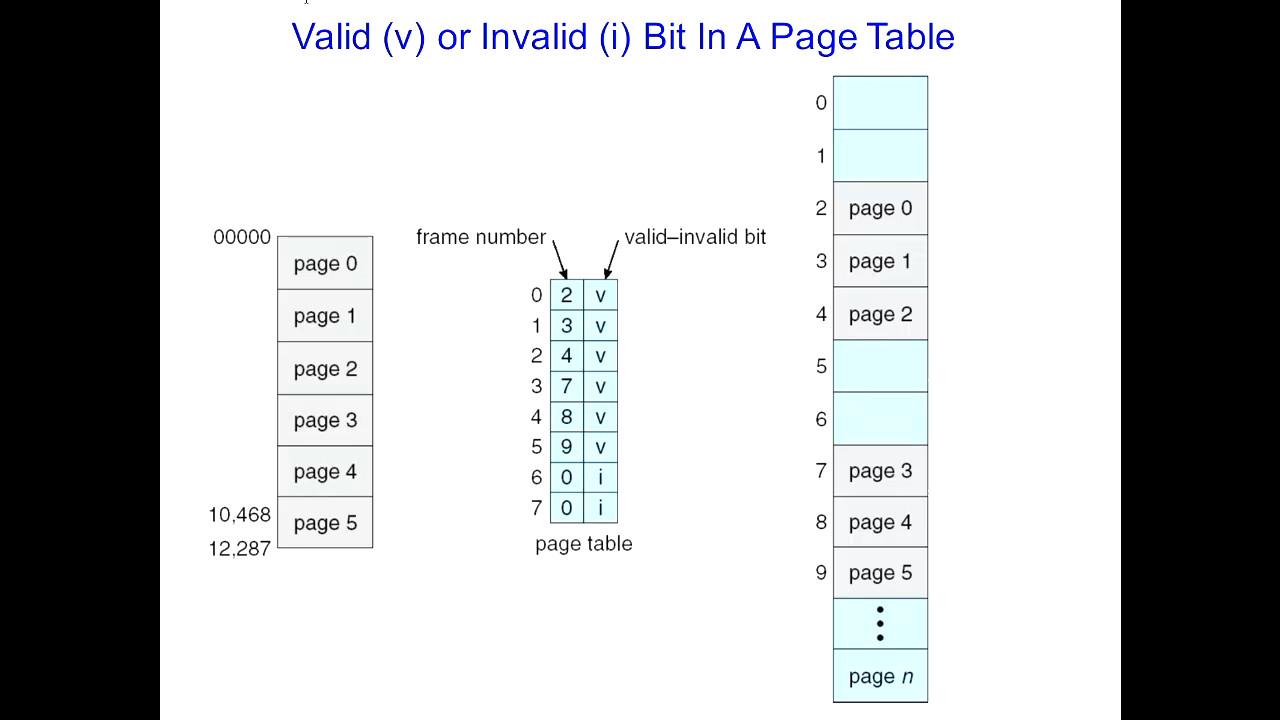
\includegraphics[height=270]{valid-or-invalid-bit-in-a-page-table.jpg}

\subsection{Shared Pages}

\textbf{Shared Pages}
\begin{itemize}
    \item \emph{Shared Code}
        \begin{itemize}
            \item One copy of read-only (\emph{re-entrant}) code shared among processes
                (i.e.\ text editors, compilers, window systems).
            \item Similar to multiple threads sharing the same process space.
            \item Also useful for interprocess communication if sharing or read-write
                pages is allowed.
        \end{itemize}
    \item \emph{Private code and data}
        \begin{itemize}
            \item Each process keeps a separate copy of the data.
            \item The pages for the private code and data can appear anywhere in the logical
                address space.
        \end{itemize}
\end{itemize}

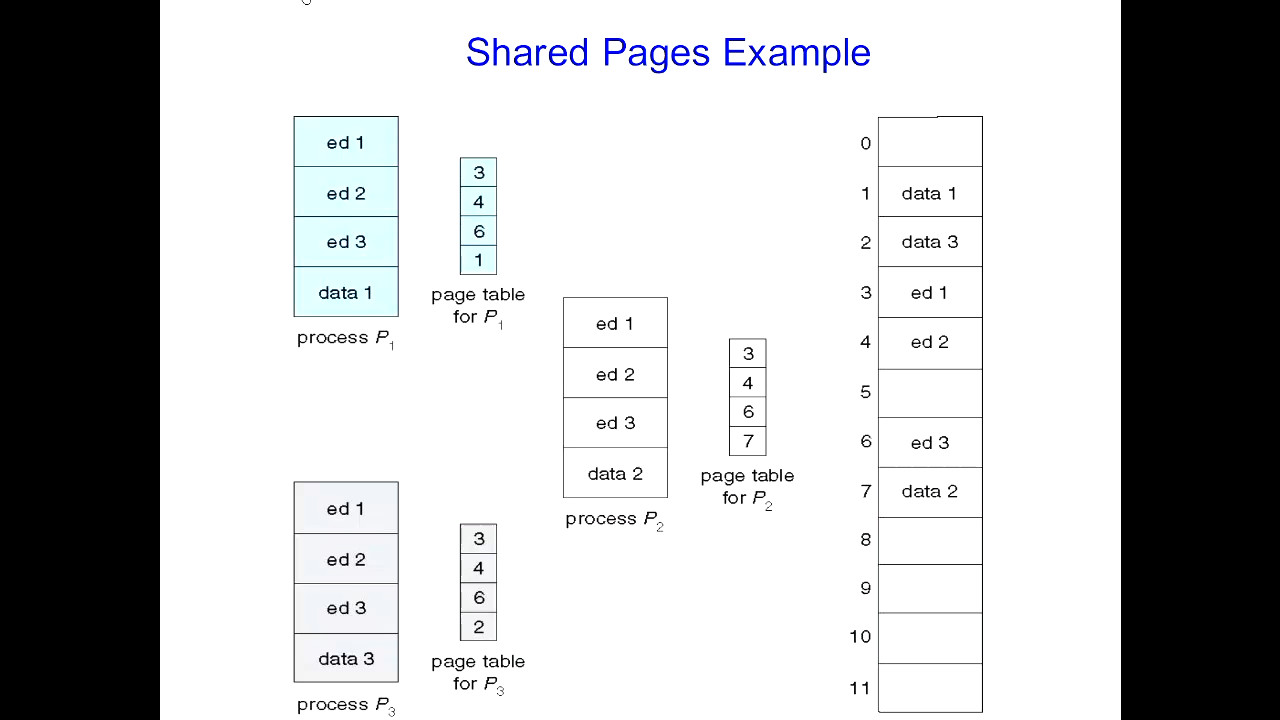
\includegraphics[height=270]{shared-pages-example.jpg}

\textbf{Structure of the Page Table}
\begin{itemize}
    \item Memory structures for paging can get huge using straightforward methods
        \begin{itemize}
            \item Consider 32-bit logical address space as on modern computers
            \item Page size of 4KB ($2^{12}$)
            \item Page table would have 1 million entries ($\frac{2^{32}}{2^{12}}$)
            \item If each entry is 4 bytes $\implies$ 4MB of of physical address space /
                memory for page table alone.
                \begin{itemize}
                    \item That amount of memory used to cost a lot
                    \item Don't want to allocate that contiguously in main memory.
                \end{itemize}
        \end{itemize}
    \item Hierarchical paging
    \item Hashed page tables
    \item Inverted page tables
\end{itemize}

\subsection{Hierarchical Pages}
\begin{itemize}
    \item Break up the logical address space into multiple page tables
    \item A simple technique is a two-level page table
    \item We then page the page table
\end{itemize}

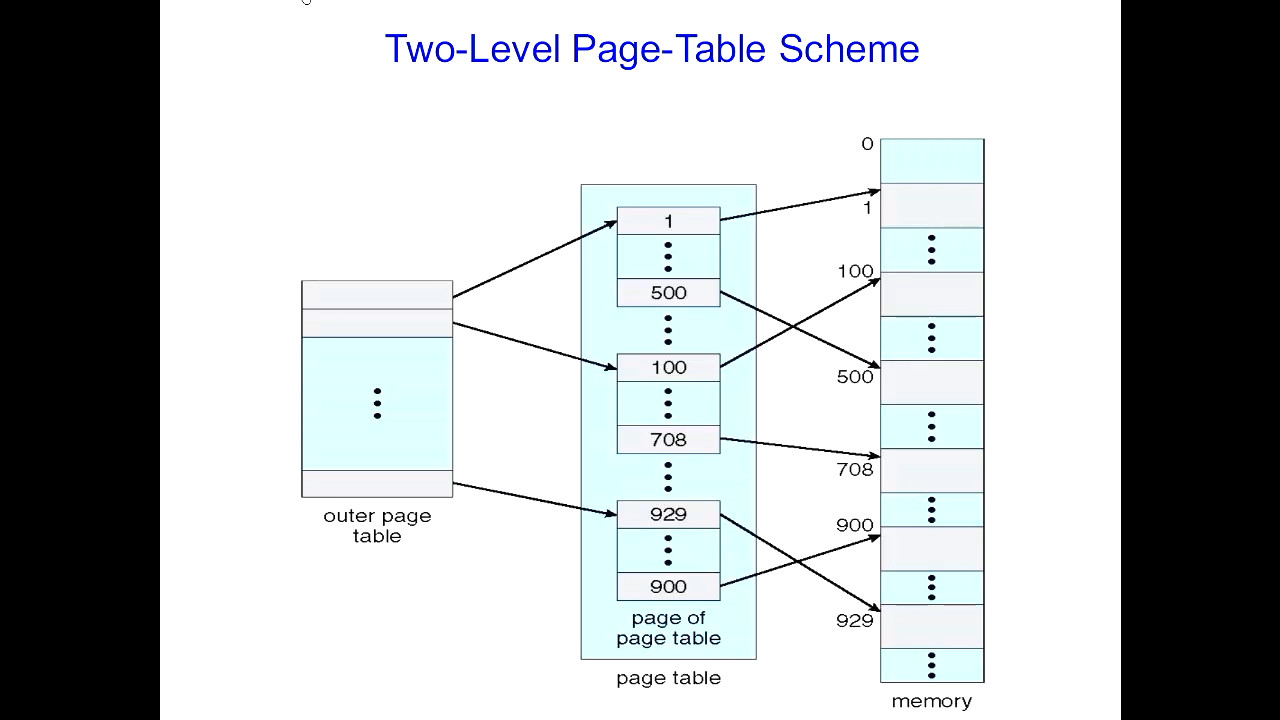
\includegraphics[height=270]{two-level-page-table-scheme.jpg}

\textbf{Two-level paging example}
\begin{itemize}
    \item A logical address (on 32-bit machines with 1K page size) is divided into:
        \begin{itemize}
            \item a page number consisting of 22 bits
            \item a page offset consisting of 10 bits
        \end{itemize}
    \item Since the page table is paged, the page number is further divided into:
        \begin{itemize}
            \item a 12-bit page number
            \item a 10-bit page offset
        \end{itemize}
    \item Thus a logical address is as follows

        \begin{tabular}{r c c}
            \toprule
            page number &       & page offset \\
            \midrule
            $p_1$       & $p_2$ & $d$ \\
            12          & 10    & 10 \\
            \bottomrule
        \end{tabular}

        where $p_1$ is an index into the outer page table, and $p_2$ is the displacement
        within the page of the inner page table.
    \item Known as \emph{forward-mapped page table}.
\end{itemize}

\textbf{64-bit logical address space}
\begin{itemize}
    \item Even two-level paging scheme not sufficient
    \item If page size is 4KB ($2^{12}$)
        \begin{itemize}
            \item Then page table has $2^{52}$ entries
            \item If two level scheme, inner page tables could be $2^{10}$ 4-byte entries
            \item Addresses would look like

                \begin{tabular}{c c c}
                    \toprule
                    outer page         & inner page & page offset \\
                    \midrule
                    $p_1$              & $p_2$      & $d$ \\
                    42                 & 10         & 12 \\
                    \bottomrule
                \end{tabular}

            \item Outer page table has $2^{42}$ entries or $2^{44}$ bytes
            \item One solution is to add a second outer page table
            \item But in the following example, the second outer page table is still
                $2^{34}$ bytes in size,
                \begin{itemize}
                    \item And possibly 4 memory access to get one physical memory location.
                \end{itemize}
        \end{itemize}
\end{itemize}

\subsection{Hashed Pages}

\begin{itemize}
    \item Common in address spaces $>$ 32 bits
    \item The virtual page number is hashed into a page table
        \begin{itemize}
            \item This page table contains a chain of elements hashing to the same location
        \end{itemize}
    \item Each element contains
        \begin{enumerate}
            \item the virtual page number
            \item the value of the mapped page frame
            \item a pointer to the next element
        \end{enumerate}
    \item Virtual page numbers are compared in this chain searching for a match
        \begin{itemize}
            \item If a match is found, the corresponding physical frame is extracted.
        \end{itemize}
    \item Variation for 64-bit addresses is \emph{clustered page tables}
        \begin{itemize}
            \item Similar to hashed but each entry refers to several pages (such as 16)
                rather than 1.
            \item Especially useful for \emph{sparse} address spaces (where memory references
                are non-contiguous and scattered).
        \end{itemize}
\end{itemize}

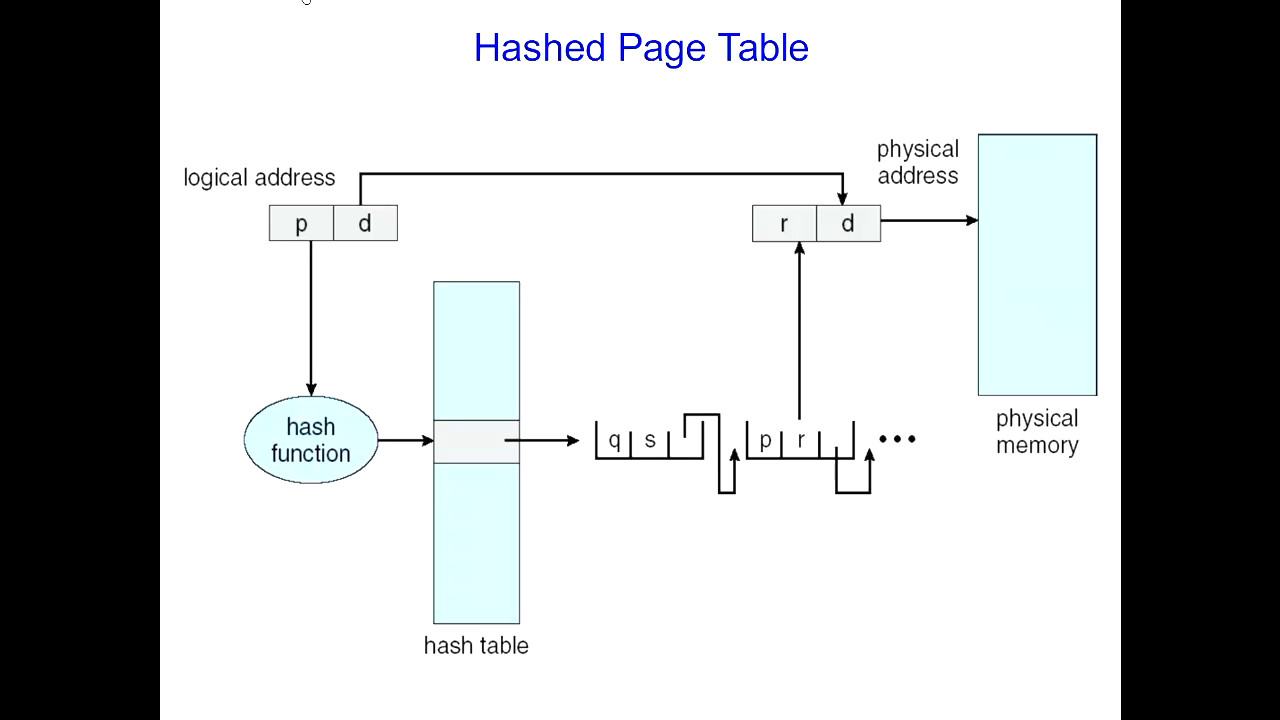
\includegraphics[height=270]{hashed-page-table.jpg}

\subsection{Inverted Pages}
\begin{itemize}
    \item Rather than each process having a page table and keeping track of all possible
        logical pages,
        \begin{itemize}
            \item track all physical pages.
        \end{itemize}
    \item One entry for each real page of memory.
    \item Entry consists of
        \begin{itemize}
            \item the virtual address of the page stored in that real memory location,
            \item information about the process that owns that page.
        \end{itemize}
    \item Decreases memory needed to store each page table
        \begin{itemize}
            \item but increases time needed to search the table when a page reference occurs.
        \end{itemize}
    \item Use hash table to limit the search to one/few page-table entries
        \begin{itemize}
            \item TLB can accelerate access.
        \end{itemize}
    \item But how to implement shared memory?
        \begin{itemize}
            \item One mapping of a virtual address to the shared physical address.
        \end{itemize}
\end{itemize}

\subsection{Uses}
\textbf{Functionality enhanced by page tables}
\begin{itemize}
    \item Code (instructions) is read-only
        \begin{itemize}
            \item A bad pointer can't change the program code
        \end{itemize}
    \item Dereferencing a null pointer is an error caught by hardware
        \begin{itemize}
            \item Don't use the first page of the virtual address space --- mark it as
                invalid --- so references to address 0 cause an interrupt.
        \end{itemize}
    \item Inter-process memory protection
        \begin{itemize}
            \item My address XYZ is different to your address XYZ
        \end{itemize}
    \item Shared libraries
        \begin{itemize}
            \item All running C programs use libc
            \item Have only one (partial) copy in physical memory, not one per process
            \item All page table entries mapping libc point to the same set of physical frames
                \begin{itemize}
                    \item DLLs in Windows
                \end{itemize}
        \end{itemize}
    \item Generalising the use of ``shared memory''
        \begin{itemize}
            \item Regions of two separate processes' address spaces map to the same physical
                frames
            \item Faster inter-process communication
                \begin{itemize}
                    \item just read/write from/to shared memory
                        Don't have to make a syscall
                \end{itemize}
            \item Will have separate Page Table Entries (PTEs) per process, so can give
                different processes different access rights
                \begin{itemize}
                    \item E.g.\ one reader, one writer.
                \end{itemize}
        \end{itemize}
    \item Copy-on-write (CoW), e.g.\ on \texttt{fork\,()}
        \begin{itemize}
            \item Instead of copying all pages, create shared mappings of parent pages in child
                address space
                \begin{itemize}
                    \item Make shared mappings read-only for both processes
                    \item When either process writes, fault occurs, OS ``splits'' the page
                \end{itemize}
        \end{itemize}
\end{itemize}

\textbf{Less familiar uses}
\begin{itemize}
    \item Memory-mapped files
        \begin{itemize}
            \item instead of using open, read, write, close
                \begin{itemize}
                    \item ``map'' a file into a region of the virtual address space
                        \begin{itemize}
                            \item e.g.\ into region with base $X$
                        \end{itemize}
                    \item accessing virtual address $X+N$ refers to offset $N$ in file
                    \item initially, all pages in mapped region marked as invalid
                \end{itemize}
            \item OS reads a page from file whenever invalid page accessed
            \item OS writes a page to file when evicted from physical memory
                \begin{itemize}
                    \item only necessary if page is dirty.
                \end{itemize}
        \end{itemize}
\end{itemize}

\textbf{More unusual use}
\begin{itemize}
    \item Use ``soft faults''
        \begin{itemize}
            \item faults on pages that are actually in memory
            \item but whose PTE entries have artificially been marked as invalid
        \end{itemize}
    \item That idea can be used whenever it would be useful to trap on a reference to some
        data item.
        \begin{itemize}
            \item Example: debugger watchpoints
        \end{itemize}
    \item Limited by the fact that the granularity of detection is the page.
\end{itemize}

\break{}

\section{Virtual Memory}

\subsection{Virtual memory}

\textbf{Paged virtual memory}
\begin{itemize}
    \item Allows a larger logical address space than physical memory
    \item All pages of address space do not need to be in memory
        \begin{itemize}
            \item the full (used) address space on disk in page-sized blocks
            \item main memory used as a (page) cache
        \end{itemize}
    \item Needed page transferred to a free page frame
        \begin{itemize}
            \item if no free page frames, evict a page
                \begin{itemize}
                    \item evicted pages go to disk only if \emph{dirty}
                \end{itemize}
            \item Transparent to the application, except for performance
            \item Managed by hardware and OS
        \end{itemize}
    \item Traditionally called \emph{paged virtual memory}
\end{itemize}

\subsection{Page Fault}

\textbf{Page Fault}
\begin{itemize}
    \item If there is a reference to a page, first reference to that page will trap to OS:\ \\
        \emph{page fault}
\end{itemize}
\begin{enumerate}
    \item OS looks at another table to decide
        \begin{itemize}
            \item invalid reference $\implies$ abort
            \item just not in memory
        \end{itemize}
    \item Find free frame
    \item Swap page into frame via scheduled disk operation
    \item Reset tables to indicate page now in memory \\
        Set validation bit = \texttt{v}
    \item Restart the instruction that caused the page fault
\end{enumerate}

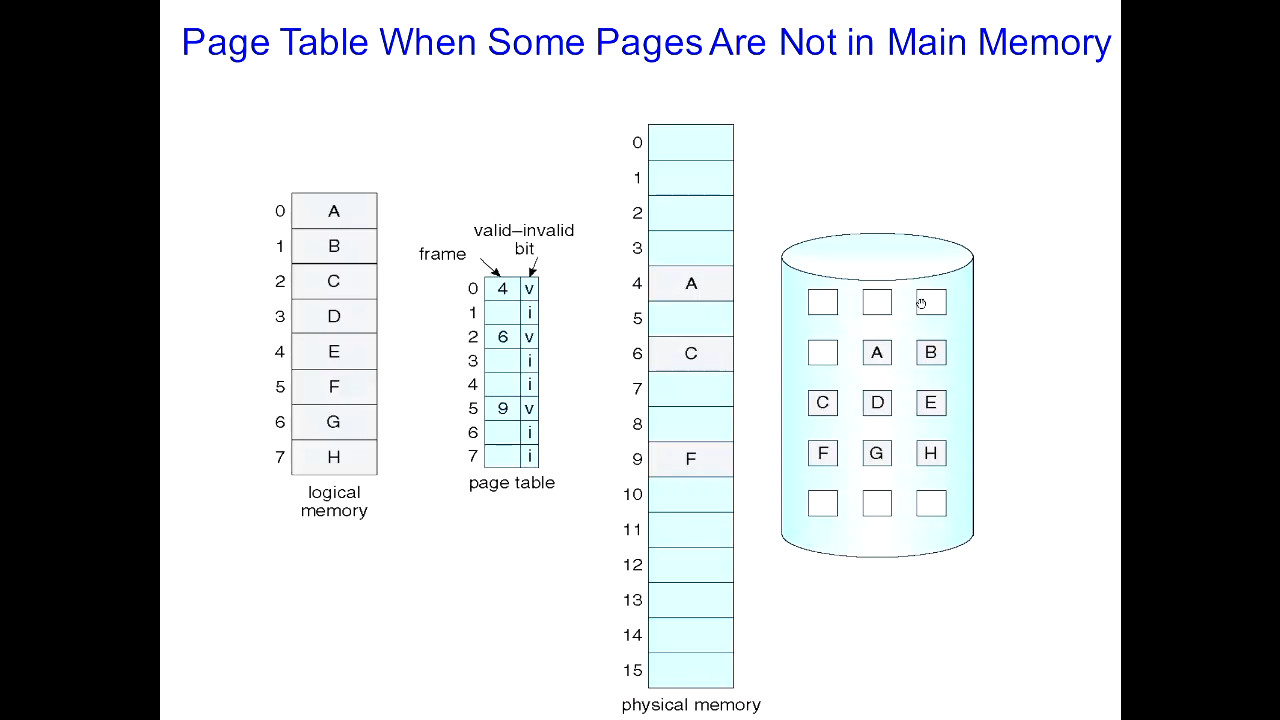
\includegraphics[height=270]{page-table-when-some-pages-are-not-in-main-memory.jpg}

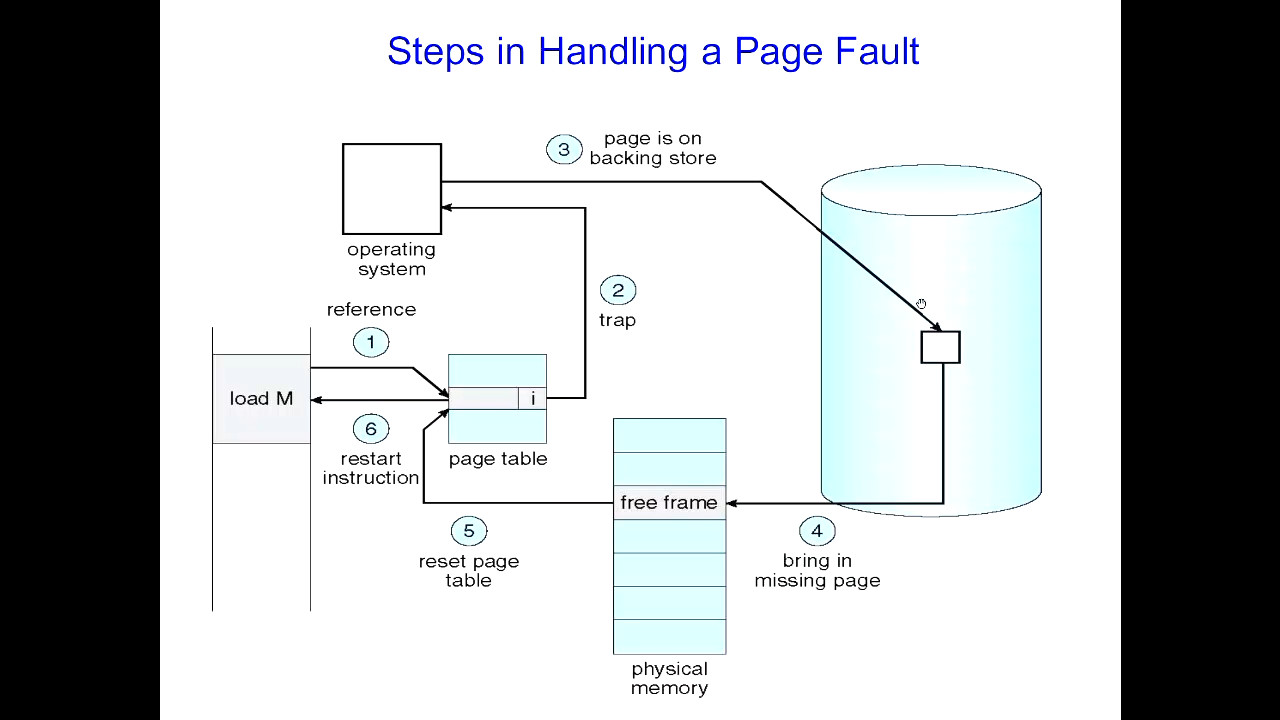
\includegraphics[height=270]{steps-in-handling-a-page-fault.jpg}

\subsection{Demand Paging}

\textbf{Demand paging}
\begin{itemize}
    \item Pages only brought into memory when referenced
        \begin{itemize}
            \item Only code/data that is needed by a process needs to be loaded
                \begin{itemize}
                    \item What's needed changes over time
                \end{itemize}
            \item Hence, it's called \emph{demand paging}
        \end{itemize}
    \item Few systems try to anticipate future needs
    \item But sometimes cluster pages
        \begin{itemize}
            \item OS keeps track of pages that should come and go together
            \item bring in all when one is referenced
            \item interface may allow programmer or compiler to identify clusters
        \end{itemize}
\end{itemize}

\subsection{Page replacement}

\textbf{Page replacement}
\begin{itemize}
    \item When you read in a page, where does it go?
        \begin{itemize}
            \item if there are free page frames, grab one
            \item if not, must evict something else
                \begin{itemize}
                    \item this is called \emph{page replacement}
                \end{itemize}
        \end{itemize}
    \item Page replacement algorithms
        \begin{itemize}
            \item try to pick a page that won't be needed in the near future
            \item try to pick a page that hasn't been modified (thus saving the disk write)
        \end{itemize}
    \item OS tries to keep a pool of free pages around
        \begin{itemize}
            \item so that allocations don't inevitably case evictions
        \end{itemize}
    \item OS tries to keep some ``clean'' pages around
        \begin{itemize}
            \item so that even if you have to evict a page, you won't have to write it
        \end{itemize}
\end{itemize}

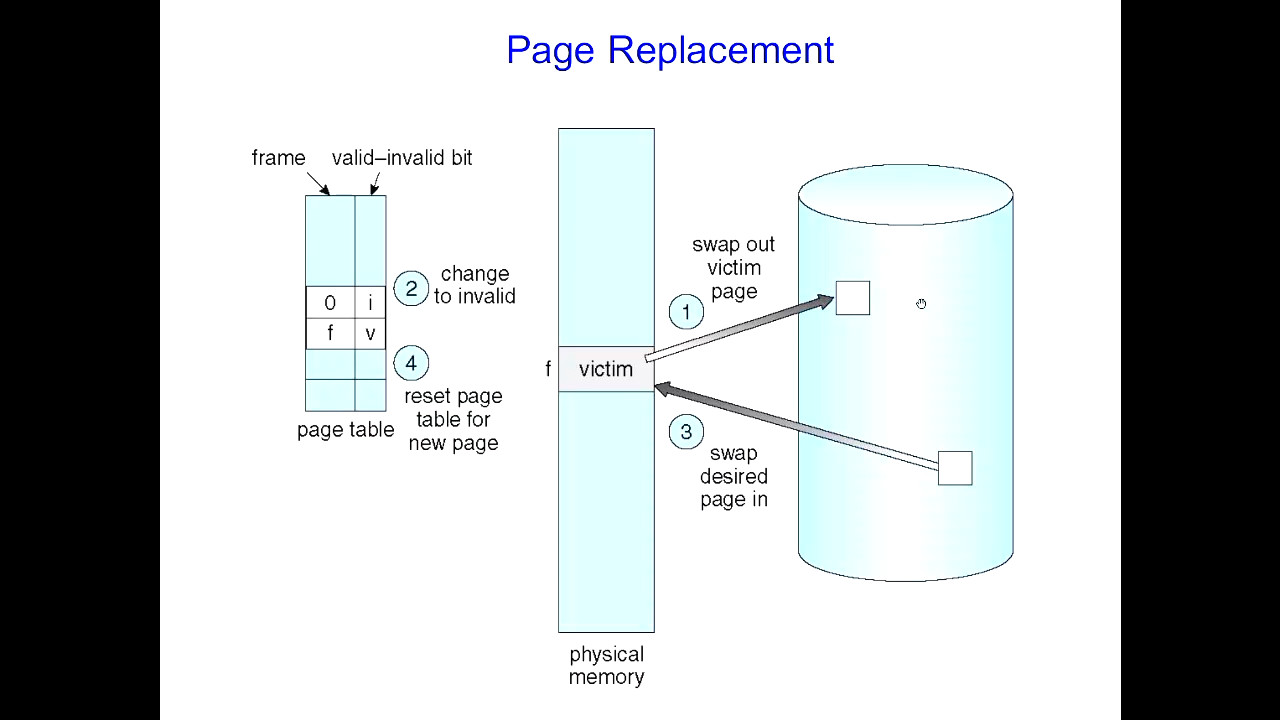
\includegraphics[height=270]{page-replacement.jpg}

\textbf{Evicting the best page}
\begin{itemize}
    \item The goal of the page replacement algorithm:
        \begin{itemize}
            \item reduce fault rate by selecting best victim page to remove
            \item the best page to evict is one that will never be touched again
            \item Belady's proof:
                \begin{itemize}
                    \item evicting the page that won't be used for the longest period of time
                        minimises the page fault rate
                \end{itemize}
        \end{itemize}
    \item Examine \emph{page replacement algorithms}
        \begin{itemize}
            \item assume that a process pages against itself
            \item using a fixed number of page frames
        \end{itemize}
    \item Number of frames available impacts page fault rate
        \begin{itemize}
            \item Note Belady's anomaly
        \end{itemize}
\end{itemize}

\subsection{Page replacement algorithms}

\textbf{First-In-First-Out (FIFO) Algorithm}
\begin{itemize}
    \item Not always the best page replacement behaviour.
\end{itemize}

\textbf{Belady's Optimal Algorithm}
\begin{itemize}
    \item Replace page that will not be used for longest period of time
    \item How do you know this?
        \begin{itemize}
            \item Can't predict the future
        \end{itemize}
    \item Used for measuring how well your algorithm performs
\end{itemize}

\textbf{Least Recently Used (LRU) algorithm}
\begin{itemize}
    \item Use past knowledge rather than future
    \item Replace page that has not been used in the most amount of time
    \item Associate time of last use with each page
    \item 12 pages --- better than FIFO but works than Belady's/OPT
    \item Generally good algorithm and frequently used
    \item But how to implement?
\end{itemize}

\textbf{Approximating LRU}
\begin{itemize}
    \item Many approximations, all use the PTE's referenced but
        \begin{itemize}
            \item keep a counter for each page
            \item at some regular interval, for each page, do:
                \begin{itemize}
                    \item if reference bit = 0, increment the counter (hasn't been used)
                    \item if reference bit = 1, zero the counter (hasn't been used)
                    \item regardless, zero bit ref
                \end{itemize}
            \item the counter will contain the number of intervals since the last reference to
                the page
                \begin{itemize}
                    \item page with largest counter is least recently used
                \end{itemize}
        \end{itemize}
    \item Some architectures don't have PTE reference bits
        \begin{itemize}
            \item can simulate reference bit using the valid bit to induce faults
        \end{itemize}
\end{itemize}

\textbf{Second-chance clock}
\begin{itemize}
    \item Not Recently Used (NRU) or Second Change
        \begin{itemize}
            \item replace page that is ``old enough''
            \item logically, arrange all physical page frames in a big circle (clock)
                \begin{itemize}
                    \item just a circular linked list
                \end{itemize}
        \end{itemize}
    \item A ``clock hand'' is used to select a good LRU candidate
        \begin{itemize}
            \item sweep through the pages in circular order like a clock
        \end{itemize}
    \item If reference bit is off, it hasn't been used recently, and we have a victim
    \item If reference bit is on, turn if off and go to next page
        \begin{itemize}
            \item arm moves quickly when pages are needed.
        \end{itemize}
\end{itemize}

\textbf{Allocation of frames among processes}
\begin{itemize}
    \item FIFO and LRU Clock each can be implemented as either \emph{local} or \emph{global}
        replacement algorithms
        \begin{itemize}
            \item local
                \begin{itemize}
                    \item each process is given a limit of pages it can use
                    \item it ``pages against itself'' (evicts its own pages)
                \end{itemize}
            \item global
                \begin{itemize}
                    \item the ``victim'' is chosen from among all page frames, regardless of
                        owner
                    \item processes' page frame allocation can vary dynamically
                \end{itemize}
        \end{itemize}
    \item Issues with local replacement?
        \begin{itemize}
            \item poor utilisation of free page frames, long access time
        \end{itemize}
    \item Issues with global replacement
        \begin{itemize}
            \item Linux uses global replacement: global thrashing.
        \end{itemize}
\end{itemize}

\subsection{Working set}

\textbf{The \emph{working set model of program behaviour}}
\begin{itemize}
    \item \emph{Working set} of a process is used to model the dynamic locality of its memory
        usage
        \begin{itemize}
            \item works set = set of pages a process currently ``needs''
            \item formally defined by Peter Denning in the 1960s.
        \end{itemize}
    \item Definition:
        \begin{itemize}
            \item WS\,$(t, w)$ = \{pages $P$ such that $P$ was referenced in the time interval
                $(t, t-w)$\}
                \begin{itemize}
                    \item $t$ time
                    \item $w$ working set \emph{window} (measured in page references)
                    \item a page in WS only if it was referenced in the last $w$ references
                \end{itemize}
        \end{itemize}
    \item Working set varies over the life of the program
        \begin{itemize}
            \item so does the \emph{working set size}
        \end{itemize}
\end{itemize}

\textbf{Working set size}
\begin{itemize}
    \item The working set size, $|\mathrm{WS}(t, w)|$
        \begin{itemize}
            \item changes with program locality
        \end{itemize}
    \item During periods of poor locality
        \begin{itemize}
            \item more pages are referenced
        \end{itemize}
    \item Within that period of time
        \begin{itemize}
            \item the working set size is larger
        \end{itemize}
    \item Intuitively, the working set must be in memory
        \begin{itemize}
            \item otherwise you'll experience heavy faulting
            \item \emph{thrashing}
        \end{itemize}
\end{itemize}

\textbf{Hypothetical Working Set Algorithm}
\begin{itemize}
    \item Estimate $|\mathrm{WS}(0, w)|$ for a process
        \begin{itemize}
            \item Allow that process to start only if you can allocate it that many page frames
        \end{itemize}
    \item Use a local replacement algorithm (LRU Clock?)
        \begin{itemize}
            \item make sure that the working set are occupying the process's frames
        \end{itemize}
    \item Track each process's working set size,
        \begin{itemize}
            \item and re-allocate page frames among processes dynamically
        \end{itemize}
    \item Problem
        \begin{itemize}
            \item keep track of working set size
        \end{itemize}
    \item Use reference bit with a fixed-interval timer interrupt.
\end{itemize}

\textbf{Working Sets and Page Fault Rates}
\begin{itemize}
    \item Direct relationship between working set of a process and its page-fault rate
    \item Working set changes over time
    \item Peaks and valleys over time
\end{itemize}

\textbf{Page-Fault frequency}
\begin{itemize}
    \item More direct approach than WSS
    \item Establish ``acceptable'' \emph{page-fault frequency (PFF)} rate and use local
        replacement policy
        \begin{itemize}
            \item If actual rate too low, process loses frame
            \item If actual rate too high, process gains frame
        \end{itemize}
\end{itemize}

\subsection{Thrashing}

\textbf{Thrashing}
\begin{itemize}
    \item Thrashing
        \begin{itemize}
            \item when the system spends most of its time servicing page faults, little time
                doing useful work
        \end{itemize}
    \item Could be that there is enough memory
        \begin{itemize}
            \item but a poor replacement algorithm --- incompatible with program behaviour
        \end{itemize}
    \item Could be that memory is over-committed
        \begin{itemize}
            \item OS sees CPU poorly utilised and adds more processes
                \begin{itemize}
                    \item too many active processes
                \end{itemize}
            \item Makes problem works
        \end{itemize}
\end{itemize}

\break{}

\section{File Systems}

\subsection{Roles}

\textbf{Primary Roles of the OS (file system)}
\begin{enumerate}
    \item Hide hardware specific interface
    \item Allocate disk blocks
    \item Check permissions
    \item Understand directory file structure
    \item Maintain \emph{metadata}
    \item Performance
    \item Flexibility
\end{enumerate}

\textbf{File systems}
\begin{itemize}
    \item The concept of a file system is simple
    \item The implementation of the abstraction for secondary storage
        \begin{itemize}
            \item abstraction = files
        \end{itemize}
    \item Logical organisation of files into directories
        \begin{itemize}
            \item the directory hierarchy
        \end{itemize}
    \item Sharing of data between
        \begin{itemize}
            \item processes, people, and machines
        \end{itemize}
    \item Access control, consistency, etc.
\end{itemize}

\subsection{Files}

\textbf{Files}
\begin{itemize}
    \item A collection of data with some properties
        \begin{itemize}
            \item contents, size, owner, last read/write time, protection, etc.
        \end{itemize}
    \item File types
        \begin{itemize}
            \item understood by file system
                \begin{itemize}
                    \item device, directory, symbolic link
                \end{itemize}
            \item understood by other parts of OS or by runtime libraries
                \begin{itemize}
                    \item executable, dll, source code, object code, text file, etc.
                \end{itemize}
        \end{itemize}
    \item Type can be encoded in the file's name or contents
        \begin{itemize}
            \item windows encodes type
                \begin{itemize}
                    \item com, exe, bat, dll, jpg, mov, mp3, \dots
                \end{itemize}
        \end{itemize}
    \item Old Mac OS stored the name of the creating program along with the file
    \item Unix --- initial characters (e.g.\ #)
\end{itemize}

\textbf{Basic operations}

\begin{tabular}{l l}
    \toprule
    \emph{Unix}                    & \emph{Windows} \\
    \midrule
    \texttt{create\,(name)}        & \texttt{CreateFile\,(name, CREATE)} \\
    \texttt{open\,(Name, mode)}    & \texttt{CreateFile\,(name, OPEN)} \\
    \texttt{read\,(fd, buf, len)}  & \texttt{ReadFile\,(handle, \dots)} \\
    \texttt{write\,(fd, buf, len)} & \texttt{WriteFile\,(handle, \dots)} \\
    \texttt{sync\,(fd)}            & \texttt{FlushFileBuffers\,(handle, \dots)} \\
    \texttt{seek\,(fd)}            & \texttt{SetFilePointer\,(handle, \dots)} \\
    \texttt{close\,(fd)}           & \texttt{CloseHandle\,(handle, \dots)} \\
    \texttt{unlink\,(name)}        & \texttt{DeleteFile\,(name)} \\
    \texttt{rename\,(old, new)}    & \texttt{CopyFile\,(name)} \\
                                   & \texttt{MoveFile\,(name)} \\
                                   \bottomrule
\end{tabular}

\textbf{File access methods}
\begin{itemize}
    \item File systems provide different \emph{access methods}
        \begin{itemize}
            \item sequential access
                \begin{itemize}
                    \item read bytes one at a time, in order
                \end{itemize}
            \item direct access
                \begin{itemize}
                    \item random access given a block/byte number
                \end{itemize}
            \item record access
                \begin{itemize}
                    \item file is array of fixed- or variable-sized records
                \end{itemize}
            \item indexed access
                \begin{itemize}
                    \item one file contains an index to a record in another file
                    \item apps can find a file based on the value in that record (similar to DB)
                \end{itemize}
        \end{itemize}
    \item Why do we care about distinguishing sequential from direct access?
        \begin{itemize}
            \item what might the FS do differently in these cases?
        \end{itemize}
\end{itemize}

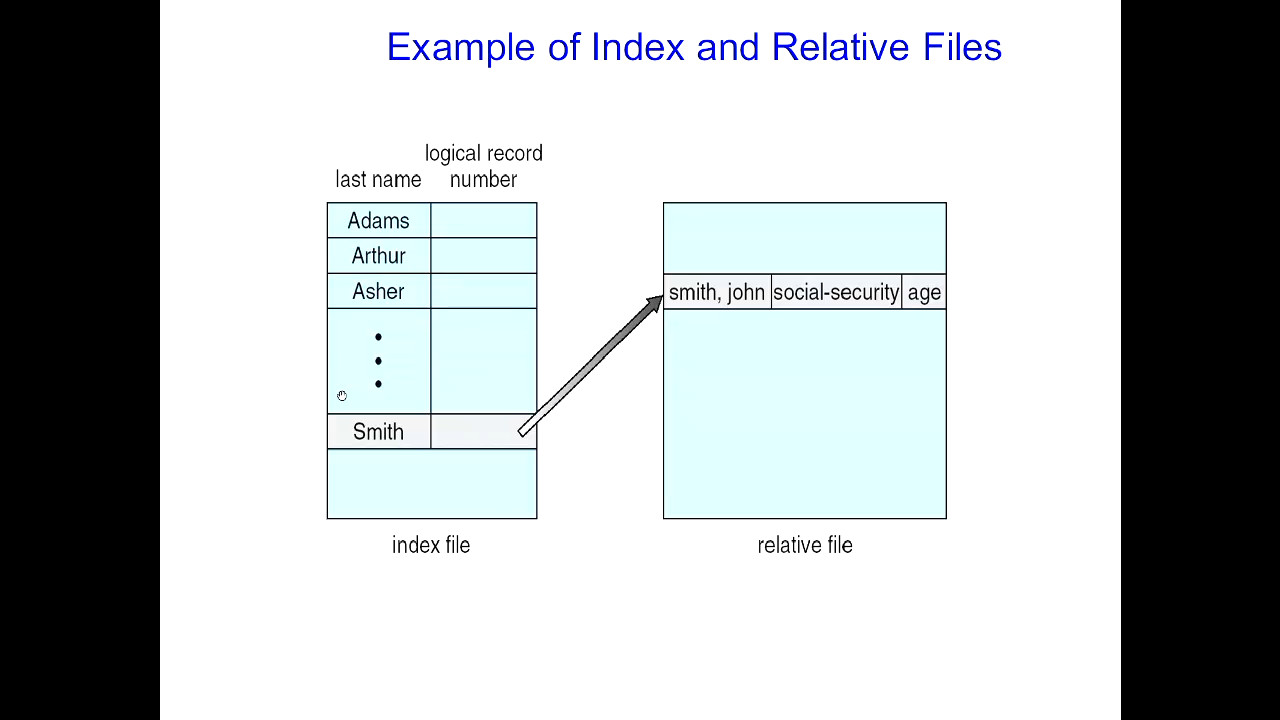
\includegraphics[height=270]{example-of-index-and-relative-files.jpg}

\subsection{Directories}

\textbf{Directories}
\begin{itemize}
    \item Directories provide:
        \begin{itemize}
            \item a way for users to organise their files
            \item a convenient file name-space for both users and file-systems
        \end{itemize}
    \item Most file-systems support multi-level directories
        \begin{itemize}
            \item naming hierarchies (\texttt{/}, \texttt{/usr}, \texttt{/usr/local},
                \texttt{/usr/local/bin}, \texttt{\dots})
        \end{itemize}
    \item Most file-systems support the notion of current directory
    \item Absolute names: fully-qualified starting from root of file-system
    \item Relative names: specified with respect to current directory
\end{itemize}

\textbf{Directory internals}
\begin{itemize}
    \item A directory is typically just a file that happens to contains special meta-data
    \item Directory
        \begin{itemize}
            \item list of (name of file, file attributes)
        \end{itemize}
    \item Attributes include such things as:
        \begin{itemize}
            \item size, protection, location on disk, creation time, access time, \dots
        \end{itemize}
    \item The directory list is usually unordered (effectively random),
        \begin{itemize}
            \item the \texttt{ls} command sorts the results for you
        \end{itemize}
\end{itemize}

\textbf{Path name translation}
\begin{itemize}
    \item You want to open \texttt{/one/two/three}
        \begin{verbatim}
    fd = open("one/two/three", O_RDWR)
        \end{verbatim}
    \item Inside the file system
        \begin{itemize}
            \item open directory \texttt{/} (well known, can always find)
            \item search the directory for \texttt{one}, get location of \texttt{one}
            \item open directory \texttt{one}, search for \texttt{two}, get location of
                \texttt{two}
            \item open directory \texttt{two}, search for \texttt{three}, got location of
                \texttt{three}
            \item open file \texttt{three}
            \item (of course, permissions are checked at each step)
        \end{itemize}
    \item File-system spends much time walking down directory paths
        \begin{itemize}
            \item this is why open is separate from read/write (session state)
            \item OS will cache prefix lookups to enhance performance
                \begin{itemize}
                    \item \texttt{/a/b}, \texttt{/a/bb}, \texttt{/a/bbb} all share the
                        \texttt{/a} prefix
                \end{itemize}
        \end{itemize}
\end{itemize}

\subsection{File Protection}

\begin{itemize}
    \item FS implements a protection system
        \begin{itemize}
            \item to control who can access a file (user)
            \item to control how they can access it (e.g.\ read, write, or exec)
        \end{itemize}
    \item Often generalised
        \begin{itemize}
            \item generalise file to \emph{objects} (the ``what'')
            \item generalise users to \emph{principals} (the ``who'', user or program)
            \item generalise read/write to \emph{actions} (the ``how,'' or operations)
        \end{itemize}
    \item Protection system dictates
        \begin{itemize}
            \item whether a given action
            \item performed by a given principal
            \item on a given object should be allowed
        \end{itemize}
    \item E.g.\ you can read or write your files, but others cannot
    \item E.g.\ you can read \texttt{/group/teaching/cs3} but you cannot write to it
\end{itemize}

\textbf{Model for representing protection}
\begin{itemize}
    \item Two different ways of thinking about it:
        \begin{itemize}
            \item access control lists (ACLs)
                \begin{itemize}
                    \item for each object, keep lists of principals and principals' allowed
                        actions
                \end{itemize}
            \item capabilities
                \begin{itemize}
                    \item for each principal, keep lists of objects and principals' allowed
                        actions
                \end{itemize}
        \end{itemize}
    \item Both can be represented with the following matrix: \\
        \begin{tabular}{l l l l}
            \toprule
                             & \texttt{/etc/passwd} & \texttt{/home/gribble} & \texttt{/home/guest} \\
                             \midrule
            \texttt{root}    & \texttt{rw}          & \texttt{rw}            & \texttt{rw} \\
            \texttt{gribble} & \texttt{r}           & \texttt{rw}            & \texttt{r} \\
            \texttt{guest}   &                      &                        & \texttt{r} \\
            \bottomrule
        \end{tabular}
\end{itemize}

\textbf{ACLs v.s.\ Capabilities}
\begin{itemize}
    \item Capabilities are easy to transfer
        \begin{itemize}
            \item they are like keys: can hand them off
            \item they make haring easy
        \end{itemize}
    \item ACLs are easier to manage
        \begin{itemize}
            \item object-centric, easy to grant and revoke
                \begin{itemize}
                    \item to revoke capability, need to keep track of principals that have it
                    \item hard to do, given that principals can hand off capabilities
                \end{itemize}
        \end{itemize}
    \item ACLs grow large when object is heavily shared
        \begin{itemize}
            \item can simplify by using \emph{groups}
                \begin{itemize}
                    \item put users in groups, put groups in ACLs
                \end{itemize}
        \end{itemize}
    \item Additional benefit
        \begin{itemize}
            \item change group membership, affects \emph{all} objects that have this group in
                its ACL
        \end{itemize}
\end{itemize}

\subsection{Unix}

\textbf{The original Unix file system}
\begin{itemize}
    \item Dennis Ritchie and Ken Thompson, Bell Labs, 1969
    \item ``Unix rose from the ashes of a multi-organisational effort in the early 1960s to
        develop a dependable timesharing operating system'' --- Multics
    \item Designed for a ``workgroup'' sharing a single system
    \item Did its job well
        \begin{itemize}
            \item Although it has been stretched in many directions
        \end{itemize}
\end{itemize}

\textbf{(Old) Unix disks are divided into five parts\dots}
\begin{enumerate}
    \item Boot block \\
        can boot the system by loading from this block
    \item Superblock \\
        specifies boundaries of next 3 areas, and contains head of freelists of inodes
        and file blocks
    \item inode area \\
        contains descriptors (inodes) for each file on the disk;
        all inodes are the same size;
        head of freelist is in the superblock.
    \item File contents area \\
        fixed-size blocks; head of freelist is in the superblock
    \item Swap area \\
        holds processes that have been swapped out of memory
\end{enumerate}

\textbf{Basic file system structures}
\begin{itemize}
    \item Every file and directory is represented by an inode
        \begin{itemize}
            \item stands for ``index node''
        \end{itemize}
    \item Contains two kinds of information
        \begin{enumerate}
            \item Metadata describing the file's owner, access rights, etc.
            \item Location of the file's blocks on disk
        \end{enumerate}
\end{itemize}

\textbf{inode format}
\begin{itemize}
    \item User number
    \item Group number
    \item Protection bits
    \item Times (file last read, file last written, inode last written)
    \item File code: specifies if the inode represents a directory, and ordinary user file,
        or a ``special'' file (typically an I/O device)
    \item Size: length of file in bytes
    \item Block list: locates contents of file (in the file contents area)
    \item Link count: number of directories referencing this inode
\end{itemize}

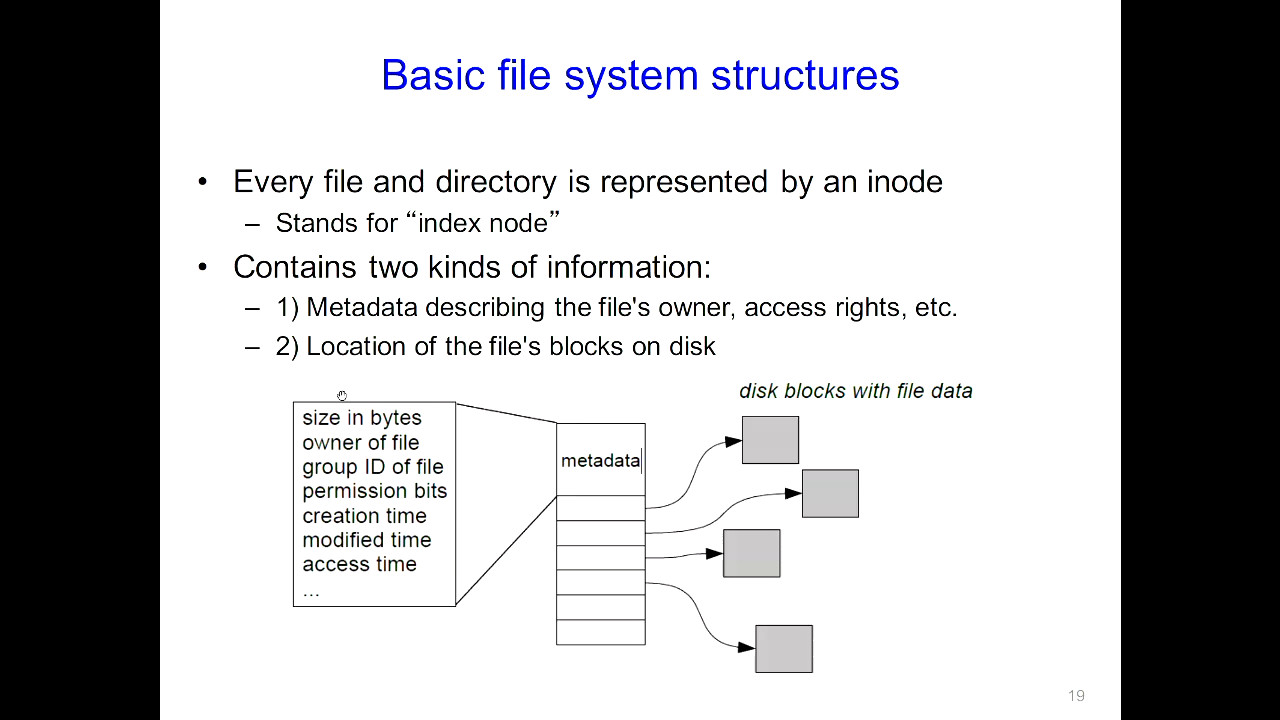
\includegraphics[height=270]{basic-file-system-structures.jpg}

\textbf{The flat (inode) file system}
\begin{itemize}
    \item Each file is known by a number, which is the number of the inode
        \begin{itemize}
            \item 1, 2, 3, etc.!
        \end{itemize}
    \item Files are created empty, and grow when extended through writes
\end{itemize}

\textbf{The tree (directory, hierarchical) file system}
\begin{itemize}
    \item A directory is a flat file of fixed-size entries
    \item Each entry consists of an inode number and a file name
        \begin{itemize}
            \item These are the contents of the directory ``file data'' itself ---
                \emph{not} the directory's inode
            \item Filenames (in Unix) are not stored in the inode at all.
        \end{itemize}
    \item Special inodes:
        \begin{itemize}
            \item inode 2 is the root directory
            \item inode 1 --- a hidden file containing all bad blocks
        \end{itemize}
\end{itemize}

\textbf{Pathname resolution}

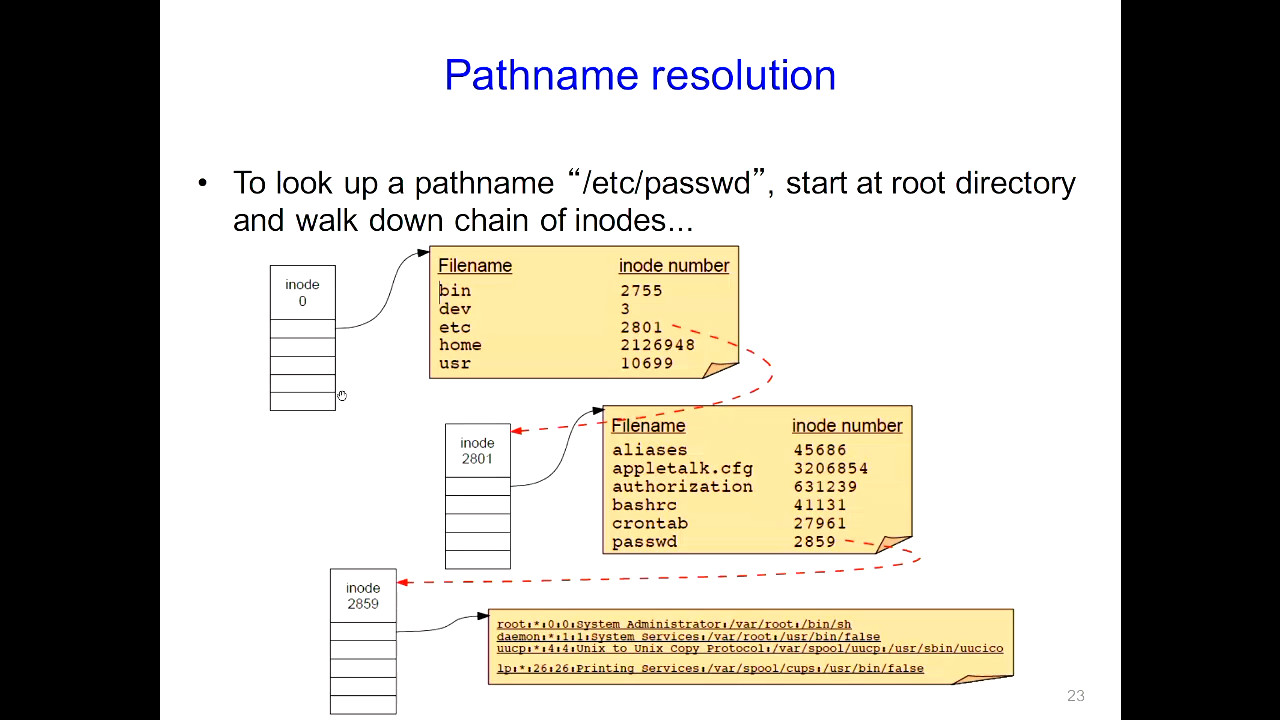
\includegraphics[height=270]{pathname-resolution.jpg}

\textbf{Locating inodes on disk}
\begin{itemize}
    \item Directories give the \emph{inode number} of a file.
        \begin{itemize}
            \item How do we find the inode itself on disk?
        \end{itemize}
    \item Basic idea: Top part of filesystem contains \emph{all} of the inodes
        \begin{itemize}
            \item inode number is just the ``index'' of the inode
        \end{itemize}
    \item Easy to compute the block address of a given inode:
        \begin{verbatim}
    block_addr(inode_num) = block_offset_of_first_inode + (inode_num * inode_size)
        \end{verbatim}
    \item This implies that a filesystem has a fixed number of potential inodes
        \begin{itemize}
            \item this number is generally set when the filesystem is created
        \end{itemize}
    \item The superblock stores important metatdata on filesystem layout,
        list of free blocks, etc.
\end{itemize}

\textbf{Directory issues}
\begin{itemize}
    \item Directories map filenames to inode numbers
    \item We can create multiple pointers to the same inode in different directories
        \begin{itemize}
            \item or even the same directory with different filenames.
        \end{itemize}
    \item In Unix, this is called a \emph{hard link} and can be done using \texttt{ln}
    \item \texttt{/home/foo} and \texttt{/tmp/foo} now refer to the same file on disk
\end{itemize}

\textbf{How should we organise blocks on a disk?}
\begin{itemize}
    \item Very simple policy: A file consists of linked blocks
        \begin{itemize}
            \item inode points to the first block of the file;
            \item each block points to the next block in the file (just a linked list on  disk)
        \end{itemize}
    \item Indexed files
        \begin{itemize}
            \item inode contains a list of block numbers containing the file:
            \item array is allocated when the file is created.
        \end{itemize}
\end{itemize}

\textbf{The ``block list'' portion of the inode (Unix Version 7)}
\begin{itemize}
    \item Points to blocks in the file contents area
    \item Must be able to represent very small and very large files.
    \item Each inode contains 13 block pointers
        \begin{itemize}
            \item first 10 are \emph{direct pointers} (pointers to 512B blocks of file data)
            \item then single, double, and triple indirect pointers
        \end{itemize}
\end{itemize}

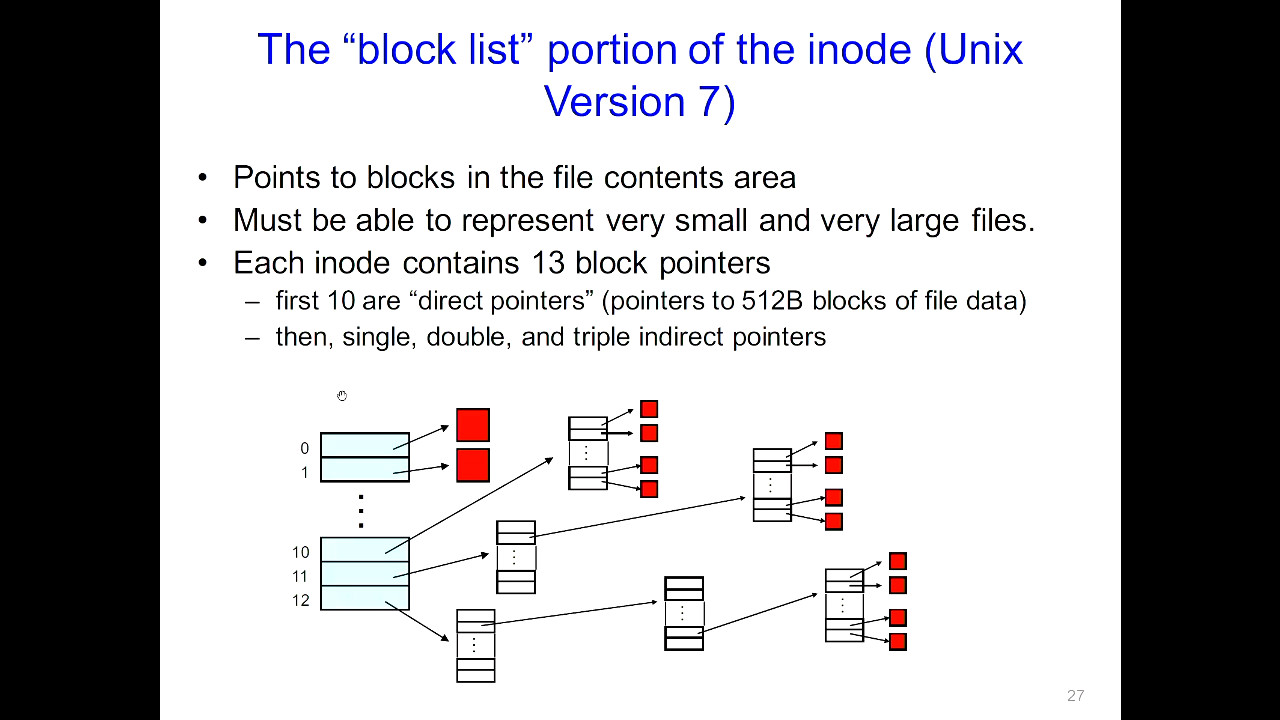
\includegraphics[height=270]{the-block-list-portion-of-the-inode.jpg}

\textbf{File Size}
\begin{itemize}
    \item Only occupies $13 \times 4$B in the inode
    \item Can get to $10 \times 512$B = a 5120B file directly
        \begin{itemize}
            \item (10 direct pointers, blocks in the file contents area are 512B)
        \end{itemize}
    \item Can get to 128 $\times$ 512B = an additional 65KB with a single indirect reference
        \begin{itemize}
            \item (the 11th pointer in the inode gets you to a 512B block in the file
                contents area that contains 128 4B pointers to blocks holding file data)
        \end{itemize}
    \item Can get to 128 $\times$ 128 $\times$ 512B = an additional 8MB with a double
        indirect reference
        \begin{itemize}
            \item (the 12th pointer in the inode gets you to a 512B block in the file contents
                area that contains 128 4B pointers to 512B blocks in the file contents area
                that contains 128 4B pointers to 512B blocks holding file data)
        \end{itemize}
    \item Can get to 128 $\times$ 128 $\times$ 128 $\times$ 512B = an additional 1GB with a
        triple indirect reference
    \item Maximum file size is a little over 1GB+
\end{itemize}

\textbf{Update File Size}
\begin{itemize}
    \item A later version of Bell Labs Unix utilised 12 direct pointers, rather than 10
    \item Berkeley Unix went to 1KB block sizes
        \begin{itemize}
            \item What's the effect on the maximum file size?
                \begin{itemize}
                    \item $256 \times 256 \times 256 \times 1\mathrm{K}$ = 17GB + a smidge
                \end{itemize}
        \end{itemize}
    \item Subsequently went to to 4KB blocks
        \begin{itemize}
            \item 1K $\times$ 1K $\times$ 1K $\times$ 4K = 4TB
        \end{itemize}
\end{itemize}

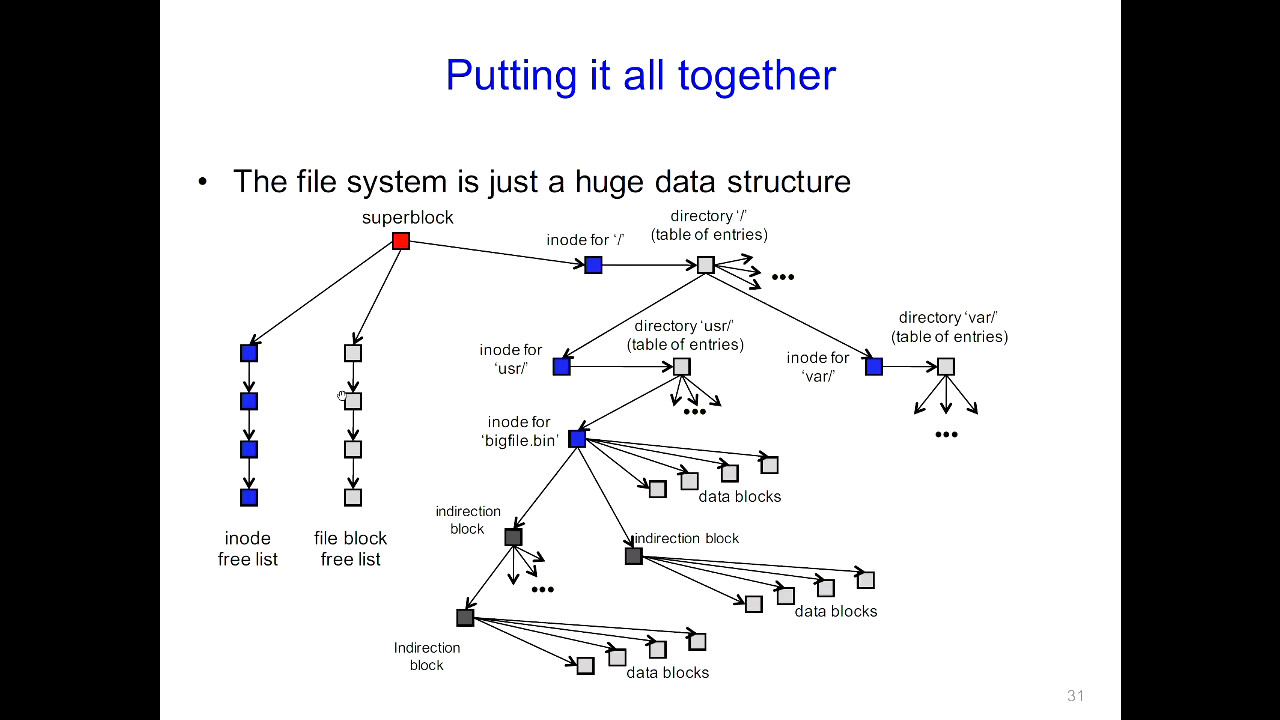
\includegraphics[height=270]{putting-it-all-together.jpg}

\textbf{File system layout}
\begin{itemize}
    \item One important goal of a filesystem is to lay this data structure out on disk
        \begin{itemize}
            \item keep in mind the physical characteristics of the disk
            \item seeks are expensive
            \item characteristics of the workload
                \begin{itemize}
                    \item locality across files within a directory
                    \item sequential access to many files
                \end{itemize}
        \end{itemize}
    \item Old Unix's layout is very inefficient
        \begin{itemize}
            \item constantly seeking
                \begin{itemize}
                    \item between inode area and data block area
                    \item as traverse filesystem, or sequentially read files
                \end{itemize}
        \end{itemize}
    \item Newer file systems are smarter
    \item Newer storage devices (SSDs) change the constraints
\end{itemize}

\break{}

\section{Virtualisation}

\textbf{Introduction}
\begin{itemize}
    \item Virtualisation is the process of creating a \emph{virtual} version of a \emph{physical}
        object.
    \item In computing, \emph{hardware virtualisation} is the process of creating a virtual
        version of real hardware.
    \item This virtual hardware can be used to run a complete OS.\
\end{itemize}

\textbf{Terminology}
\begin{itemize}
    \item \emph{Virtual Machine}:
        A \emph{virtual} representation of a \emph{physical} machine
        \begin{itemize}
            \item Not to be confused with a \emph{Java Virtual Machine} or the \emph{CLR} (.NET)
        \end{itemize}
    \item \emph{Virtual Machine Monitor} or \emph{Hypervisor}:
        A software application that monitors and manages running virtual machines.
    \item \emph{Host Machine}:
        The \emph{physical} machine that a \emph{virtual} machine is running on.
    \item \emph{Guest Machine}:
        The \emph{virtual} machine, running on the \emph{host} machine.
\end{itemize}

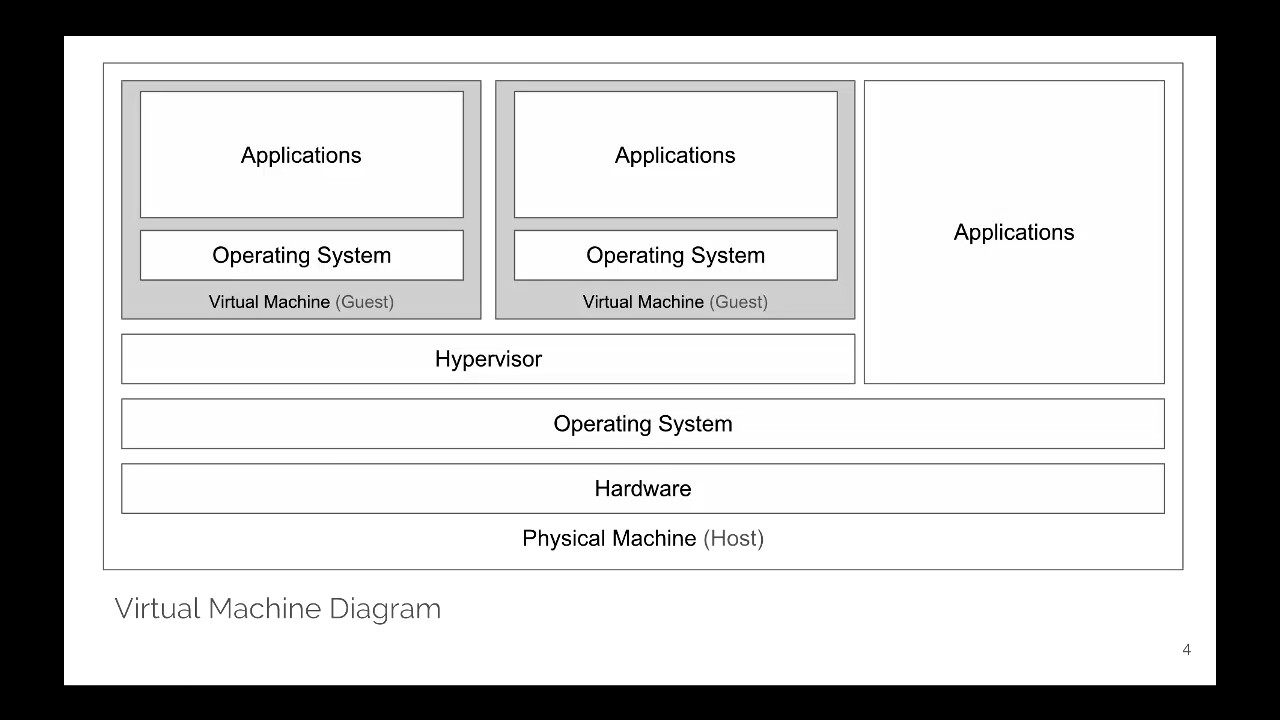
\includegraphics[height=270]{virtual-machine-diagram.jpg}

\textbf{Virtual Machine Monitor (Hypervisor)}
\begin{itemize}
    \item The VMM is in charge of running the \emph{virtual machines}.
    \item There are two main types of VMM:\
        \begin{itemize}
            \item Type 1: \emph{Native} \\
                run directly on the host machine, and share out resources (such as
                memory and devices) between guest machines.
                (E.g.\ XEN, Oracle VM Server.)
            \item Type 2: \emph{Hosted} \\
                run as an application inside an OS, and support virtual machines running as
                individual processes.
                (E.g.\ VirtualBox, Parallels Desktop, QEMU.)
        \end{itemize}
\end{itemize}

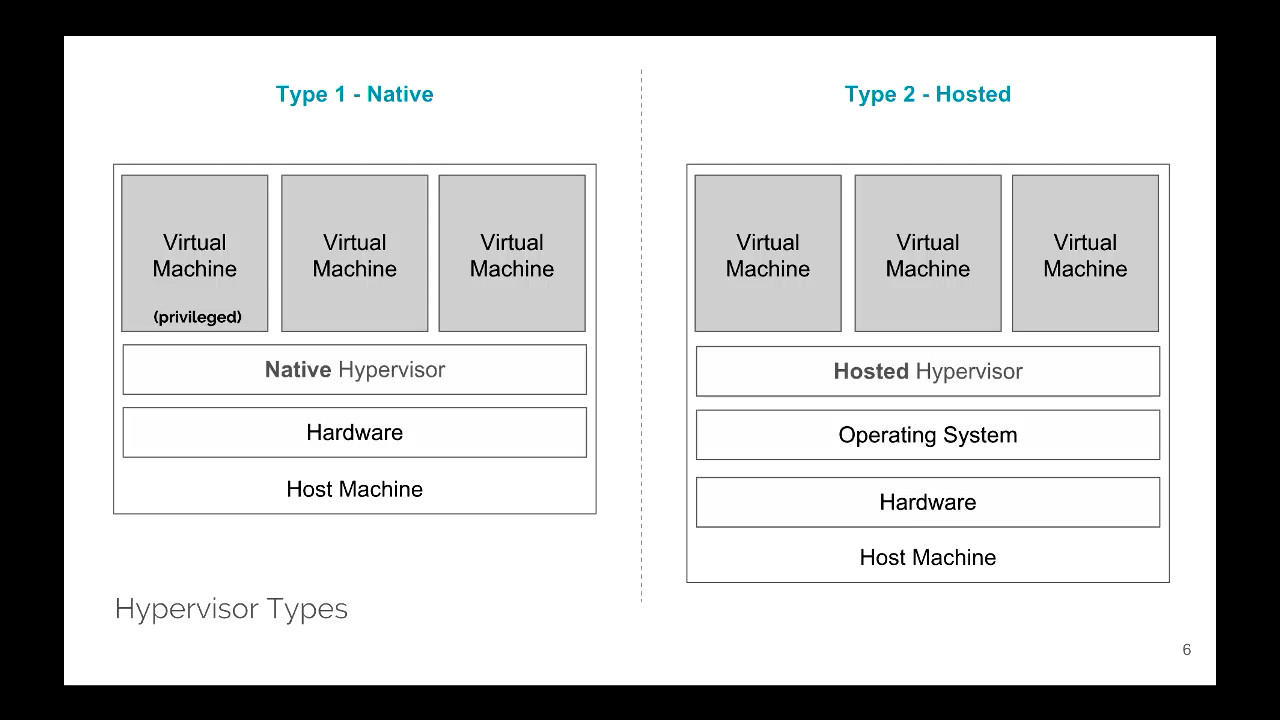
\includegraphics[height=270]{hypervisor-types.jpg}

\textbf{Uses of Virtualisation}
\begin{itemize}
    \item \emph{Personal} (e.g.\ Parallels Desktop / VirtualBox)
        \begin{itemize}
            \item Running multiple OSs on one host, without the inconvenience of rebooting.
            \item E.g.\ running Windows inside OS X.
            \item Some hypervisors support \emph{seamless integration}.
        \end{itemize}
    \item \emph{Technical} (e.g.\ QEMU as used in the coursework)
        \begin{itemize}
            \item OS / Hardware Design
            \item Kernel Debugging/Testing
            \item Prototyping new architectures / architectural features
        \end{itemize}
    \item \emph{Commercial} (e.g.\ XEN/VMWare)
        \begin{itemize}
            \item Data centre server consolidation
            \item High availability / Migration
        \end{itemize}
\end{itemize}

\textbf{Types of Virtualisation}
\begin{itemize}
    \item Software emulation
        \begin{itemize}
            \item Maximum flexibility for virtualisation, but very slow to run (high overhead).
            \item Each guest instruction is emulated (can use \emph{binary translation} for
                speed-up).,
        \end{itemize}
    \item Containers/Namespaces
        \begin{itemize}
            \item Isolate processes / groups of processes within a single OS, e.g.\ Docker.
        \end{itemize}
    \item Full System or Hardware Virtualisation
        \begin{itemize}
            \item Guest machine is the \emph{same} architecture as the host machine,
                e.g.\ Intel x86 on Intel x86.
        \end{itemize}
    \item Cross-architecture Virtualisation
        \begin{itemize}
            \item Guest machine has a \emph{different} architecture to the host machine,
                e.g.\ ARM on Intel X86.
            \item Must use \emph{software emulation} to do this.
        \end{itemize}
\end{itemize}

\textbf{Popek and Goldberg Requirements for virtualisation}

Paper published in 1974 that laid the foundations for hardware virtualisation,
and formalised the requirements for an architecture to be \emph{virtualisable}.

Three main properties for a virtual machine
\begin{enumerate}
    \item Efficiency
        \begin{itemize}
            \item The majority of guest instructions are executed directly on the host machine.
        \end{itemize}
    \item Resource control
        \begin{itemize}
            \item The virtual machine monitor must remain in control of all machine resources.
        \end{itemize}
    \item Equivalence
        \begin{itemize}
            \item The virtual machine must behave in a way that is indistinguishable from if it
                was running as a physical machine.
        \end{itemize}
\end{enumerate}

\textbf{Efficiency}
\begin{itemize}
    \item \emph{``All innocuous instructions are executed by the hardware directly,
        with no intervention at all on the part of the control program.''}
    \item Normal guest machine instructions should be executed directly on the processor.
        System instructions need to be emulated by the VMM.\
\end{itemize}

\textbf{Resource control}
\begin{itemize}
    \item \emph{``It must be impossible for that arbitrary program to affect the system
            resources, i.e.\ memory available to it;
        the allocator of the control program is to be invoked upon any attempt.''}
    \item The virtual machine should not be able to affect the host machine in any adverse way.
        The host machine should remain in control of all physical resources,
        sharing them out to guest machines.
\end{itemize}

\textbf{Equivalence}
\begin{itemize}
    \item \emph{``Any program $K$ executing with a control program resident,
            with two possible exceptions,
            performs in a manner indistinguishable from the case when the control program
            did not exist and $K$ had whatever freedom of access to privileged instructions
        that the programmer had intended.''}
    \item A formal way of saying that the OS running on a virtual machine should believe it is
        running on a physical machine, i.e.\ the behaviour of the virtual machine
        (from the guest OS' point of view) is identical to that of the corresponding physical
        machine.
    \item The two exceptions mentioned are:
        \begin{itemize}
            \item \emph{temporal latency} (some instruction sequences will take longer to run);
            \item \emph{resource availability} (physical machine resources are shared between
                virtual machines).
        \end{itemize}
\end{itemize}

\textbf{Methods of virtualisation}
\begin{itemize}
    \item Full software emulation
        \begin{itemize}
            \item Not permitted by \emph{Popek ad Goldberg} because it violates the
                \emph{efficiency} property.
                \begin{itemize}
                    \item Although, this no longer holds due to the advent of
                        \emph{efficient binary translation}.
                \end{itemize}
            \item Required for \emph{cross-architecture virtualisation}, as guest instructions
                cannot execute natively on the host.
        \end{itemize}
    \item Trap-and-emulate
        \begin{itemize}
            \item The guest OS runs \emph{de-privileged}, all non-privileged instructions
                execute natively on the host.
            \item All privileged instructions \emph{trap} to the VMM.\
            \item VMM \emph{emulates} these privileged operations.
            \item Guest resumes execution after emulation.
        \end{itemize}
\end{itemize}

\textbf{Virtualising x86}
\begin{itemize}
    \item Originally x86 was not ``classically'' virtualisable.
        \begin{itemize}
            \item Some privileged instructions did not \emph{trap}, and so could not be
                emulated correctly.
        \end{itemize}
    \item \emph{Interpretation} is too slow (violates \emph{efficiency})
    \item \emph{Code Patching} leaves traces of virtualisation (violates \emph{equivalency})
    \item \emph{Binary Translation} is better, but still incurs overhead.
    \item Since 2005, x86 processors now support virtualisation in hardware,
        \begin{itemize}
            \item Intel-VT
            \item AMD-V
        \end{itemize}
    \item The enables \emph{trap-and-emulate} style virtualisation.
    \item Unmodified OSs can run natively on host machines.
\end{itemize}

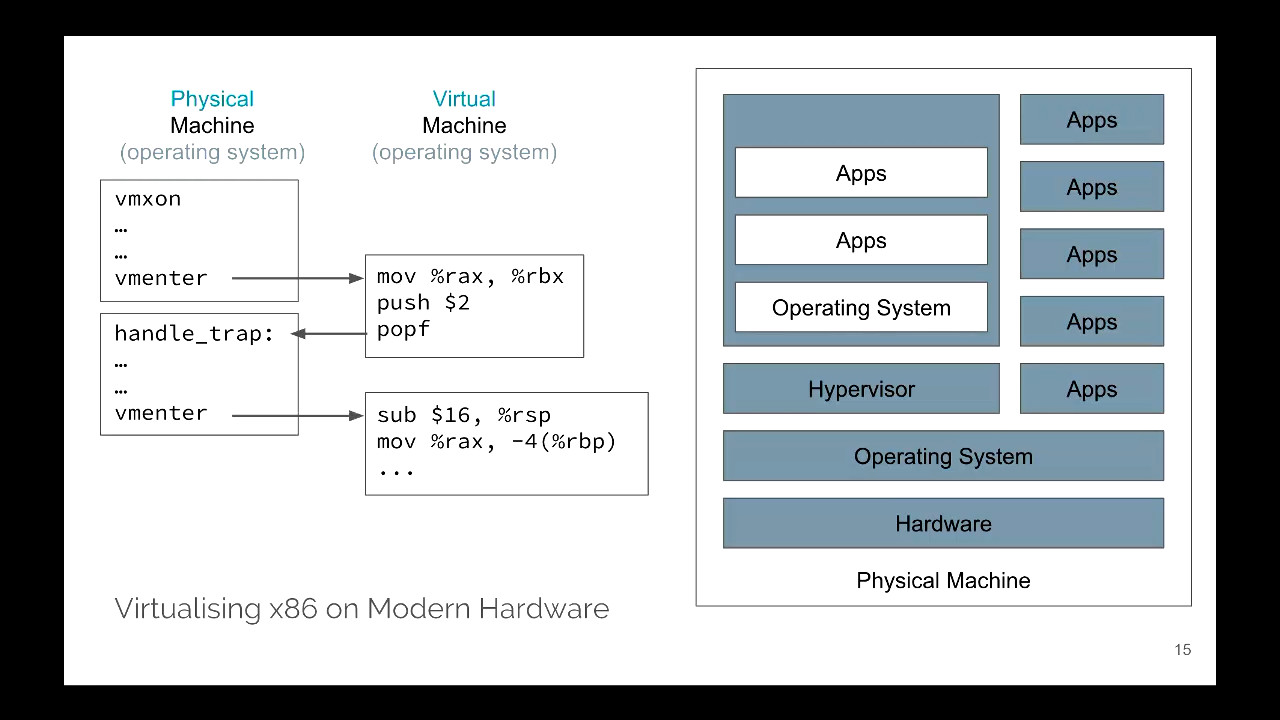
\includegraphics[height=270]{virtualising-x86-on-modern-hardware.jpg}

\textbf{Hardware acceleration for virtualisation}
\begin{itemize}
    \item Modern processors include hardware support for running virtual machines
        \begin{itemize}
            \item Intel VT-X and AMD-V for x86 processors.
            \item ARM virtualisation extensions for ARM processors.
        \end{itemize}
    \item Hardware extensions allow all guest instructions (including system instructions)
        to run natively on the processor.
    \item This works by providing an isolated view of the processor to virtual machines.
    \item OSs can then run \emph{directly} on the processor, believing they are running on
        physical hardware.
    \item Certain privileged operations \emph{trap} back to the hypervisor.
\end{itemize}

\textbf{Virtual machine access to resources}
\begin{itemize}
    \item Virtual machines need to be given access to resources such as:
        \begin{itemize}
            \item Memory
            \item Storage
            \item Networking
            \item Graphics
        \end{itemize}
    \item It is the responsibility of the VMM to share out these resources.
    \item Access to physical memory is managed by the VMM.\
    \item For an \emph{unmodified} OS, expecting a ``real'' storage device (e.g.\ a hard disk),
        the VMM must provide an \emph{emulation} of that device.
    \item Some devices may be \emph{passed straight through} to the virtual machine,
        e.g.\ dedicated \emph{network cards}.
\end{itemize}

\textbf{Paravirtualisation}
\begin{itemize}
    \item Guest OSs are \emph{aware} they are being virtualised.
    \item They \emph{co-operate} with the hypervisor to enable increased \emph{memory} and
        \emph{device} performance.
    \item They no longer \emph{trap-and-emulate}, but instead request privileged operations
        directly from the hypervisor.
    \item They can \emph{co-operate} with the hypervisor so that host memory can be more
        efficiently distributed.
        Instead of providing an \emph{emulated storage device}, the hypervisor can provide
        a \emph{paravirtualised} implementation.
    \item Typically used in \emph{data centres} for large-scale virtualisation.
\end{itemize}

\break{}

\section{Secondary Storage}

\textbf{Secondary storage}
\begin{itemize}
    \item Secondary storage:
        \begin{itemize}
            \item anything outside ``primary memory''
            \item direct execution of instructions/data retrieval via machine load/store
                \begin{itemize}
                    \item not permitted
                \end{itemize}
        \end{itemize}
    \item Characteristics:
        \begin{itemize}
            \item it's large: 250--2000GB and more
            \item it's cheap: \$0.05/GB for hard drives
        \end{itemize}
    \item Persistent: data survives power loss
        \begin{itemize}
            \item it's slow: milliseconds to access
        \end{itemize}
    \item It \emph{does} fail, if rarely
    \item Big failures:
        \begin{itemize}
            \item drive dies: Mean Time Between Failure $\sim$3 years
            \item 100K drives and MTBF is 3 years
                \begin{itemize}
                    \item that's 1 ``big failure'' every 15 minutes!
                \end{itemize}
        \end{itemize}
    \item Little failures (read/write errors, one byte in $10^{13}$)
\end{itemize}

\subsection{Disk trends}

\textbf{Disk trends}
\begin{itemize}
    \item Disk capacity, 1975--1989
        \begin{itemize}
            \item doubled every 3+ years
            \item 25\% improvement each year
            \item factor of 10 every decade
            \item \emph{Still exponential, but far less rapid than processor performance}
        \end{itemize}
    \item Disk capacity, 1990--recently
        \begin{itemize}
            \item doubling every 12 months
            \item 100\% improvement each year
            \item factor of 1000 every decade
            \item \emph{Capacity growth 10$\times$ as fast a processor performance}
        \end{itemize}
\end{itemize}

\textbf{Disk cost}
\begin{itemize}
    \item Only a few years ago, disks purchased by the megabyte
    \item Today, 1GB costs \$0.05 from Dell
        \begin{itemize}
            \item (except you have to buy in increments of 1000GB)
            \item $\implies$ 1TB costs \$50, 1PB costs \$50K
        \end{itemize}
    \item Performance analogy
        \begin{itemize}
            \item Flying an aircraft at 600mph 6 inches above the ground
            \item Reading/write a strip of postage stamps
        \end{itemize}
\end{itemize}

\subsection{Memory hierarchy}

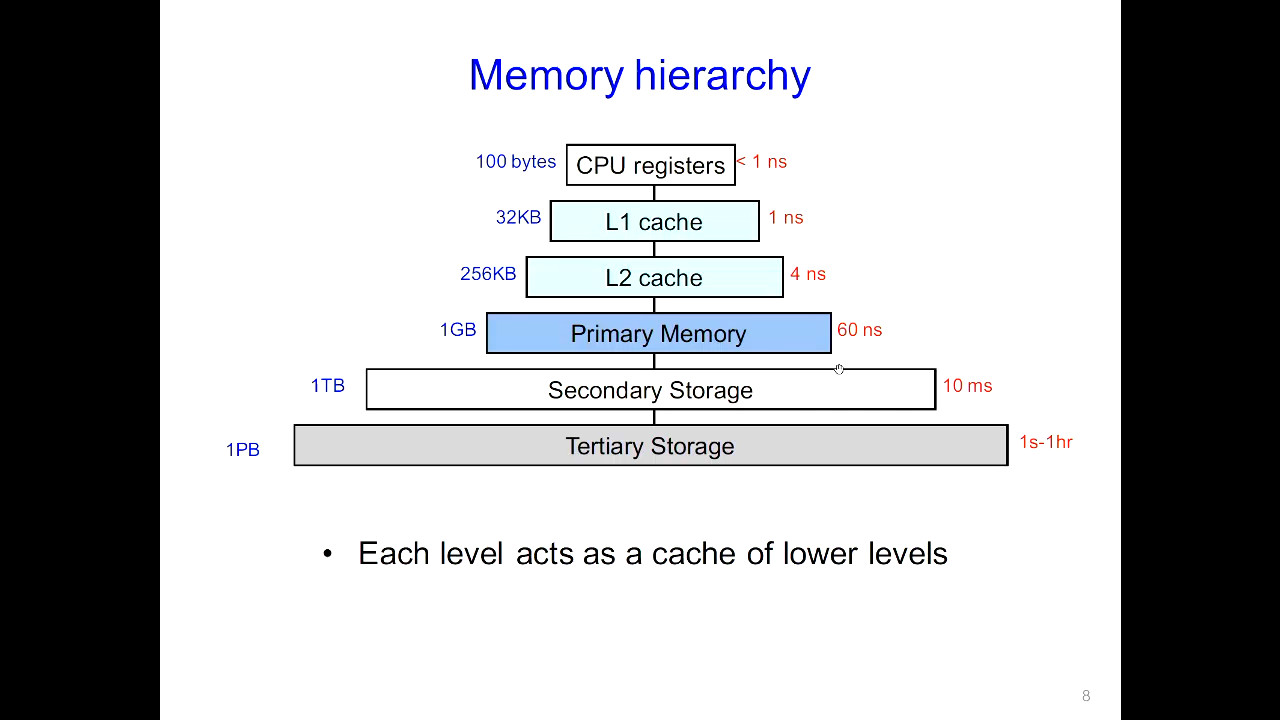
\includegraphics[height=270]{memory-hierarchy.jpg}

\textbf{Disks and the OS}
\begin{itemize}
    \item Disks are difficult devices
        \begin{itemize}
            \item errors, bad blocks, missed seeks, etc.
        \end{itemize}
    \item OS abstracts this for higher-level software
        \begin{itemize}
            \item lower-level device drivers (initiate a disk read, etc.)
            \item higher-level abstractions (file, databases, etc.)
            \item disk hardware increasingly helps with this
        \end{itemize}
    \item OS provide different levels of disk access to different clients
        \begin{itemize}
            \item physical disk block (surface, cylinder, sector)
            \item disk logical block (disk block number)
            \item file logical (filename, block or record or byte number)
        \end{itemize}
\end{itemize}

\textbf{Physical disk structure}
\begin{itemize}
    \item Disk components
        \begin{itemize}
            \item platters
            \item surfaces
            \item tracks
            \item sectors
            \item cylinders
            \item arm
            \item heads
        \end{itemize}
\end{itemize}

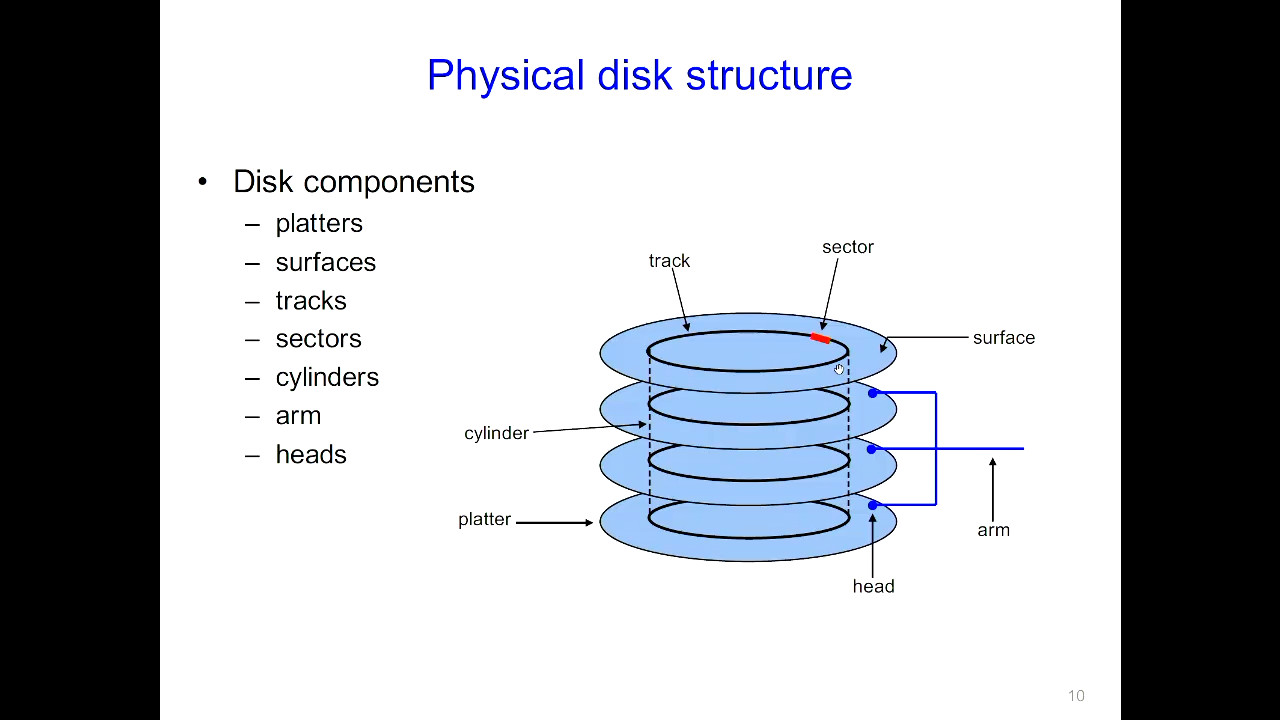
\includegraphics[height=270]{physical-disk-structure.jpg}

\textbf{Disk structure}
\begin{itemize}
    \item Disk drives are addressed as
        \begin{itemize}
            \item large 1-dimensional arrays of \emph{logical blocks}
            \item the logical block is the smallest unit of transfer
            \item low-level formatting creates \emph{logical blocks} on physical media
        \end{itemize}
    \item The 1-dimensional array of logical blocks
        \begin{itemize}
            \item is mapped onto the sectors of the disk sequentially
        \end{itemize}
    \item Sector 0 is the first sector of the first track on the outermost cylinder
        \begin{itemize}
            \item mapping proceeds in order through that track
            \item then the rest of the tracks in that cylinder
            \item then through the rest of the cylinders from outermost to innermost
        \end{itemize}
    \item Logical to physical address should be easy
        \begin{itemize}
            \item except for bad sectors
            \item non-constant number of sectors per track via constant angular velocity
        \end{itemize}
\end{itemize}

\subsection{Performance}

\textbf{Disk performance}
\begin{itemize}
    \item Performance depends on a number of steps
    \item \emph{Seek}: moving the disk arm to the correct cylinder
        \begin{itemize}
            \item depends on how fast disk arm can move
                \begin{itemize}
                    \item not diminishing quickly due to physics
                \end{itemize}
        \end{itemize}
    \item \emph{Rotation (latency)}: waiting for the sector to rotate under head
        \begin{itemize}
            \item depends on rotation rate of disk
                \begin{itemize}
                    \item rates are slowly increasing
                \end{itemize}
        \end{itemize}
    \item \emph{Transfer}: transferring data from surface to disk controller
        \begin{itemize}
            \item  then sending it back to host
            \item depends on density of bytes on disk
                \begin{itemize}
                    \item increasing, relatively quickly
                \end{itemize}
        \end{itemize}
    \item When the OS uses the disk, it tries to minimise the cost of all these steps
        \begin{itemize}
            \item particularly seeks and rotation
        \end{itemize}
\end{itemize}

\textbf{Performance}
\begin{itemize}
    \item OS may increase file block size
        \begin{itemize}
            \item in order to reduce seeking
        \end{itemize}
    \item OS may seek to co-locate ``related'' items
        \begin{itemize}
            \item in order to reduce seeking
                \begin{itemize}
                    \item blocks of the same file
                    \item data and metadata for a file
                \end{itemize}
        \end{itemize}
    \item Keep data or metadata in memory to reduce physical disk access
        \begin{itemize}
            \item Waste valuable physical memory:
        \end{itemize}
    \item If file access is sequential
        \begin{itemize}
            \item fetch blocks into memory before requested
        \end{itemize}
\end{itemize}

\subsection{Scheduling}

\textbf{Performance via disk scheduling}
\begin{itemize}
    \item Seeks are very expensive, so the OS attempts to schedule disk requests that are
        queued waiting for the disk
        \begin{itemize}
            \item FCFS (do nothing)
                \begin{itemize}
                    \item reasonable when load is low
                    \item long waiting time for long request queues
                \end{itemize}
            \item SSST (shortest seek time first)
                \begin{itemize}
                    \item minimise arm movement (seek time), maximise request rate
                    \item unfairly favours middle blocks
                \end{itemize}
            \item SCAN (elevator algorithm)
                \begin{itemize}
                    \item service requests in one direction until done, then reverse
                    \item skews wait times non-uniformly
                \end{itemize}
            \item C-SCAN
                \begin{itemize}
                    \item like scan, but only go in one direction (typewriter)
                    \item uniform wait times
                \end{itemize}
            \item C-LOOK
                \begin{itemize}
                    \item similar to C-SCAN
                    \item The arm goes only as far as the final request in each direction
                \end{itemize}
        \end{itemize}
\end{itemize}

\textbf{Selecting a Disk-Scheduling Algorithm}
\begin{itemize}
    \item SSTF is common and has a natural appeal
    \item SCAN and C-SCAN perform better for systems that place a heavy load on the disk
        \begin{itemize}
            \item  Less starvation
        \end{itemize}
    \item Performance depends on the number and types of requests
    \item Requests for disk service can be influenced by the file-allocation method
        \begin{itemize}
            \item And metadata layout
        \end{itemize}
    \item The disk-scheduling algorithm should be
        \begin{itemize}
            \item written as a separate module of the OS
            \item allowing it to be replaced with a different algorithm if neessary
        \end{itemize}
    \item Either SSTF or C-LOOK is a reasonable choice for the default algorithm
    \item What about rotational latency?
        \begin{itemize}
            \item Difficult for OS to calculate
        \end{itemize}
\end{itemize}

\textbf{Interacting with disks}
\begin{itemize}
    \item Previously
        \begin{itemize}
            \item OS would specify cylinder number, sector number, surface number, transfer size
                \begin{itemize}
                    \item i.e.\ OS needs to know all the disk parameters
                \end{itemize}
        \end{itemize}
    \item Modern disks more complex
        \begin{itemize}
            \item not all sectors are the same size, sectors are remapped, \dots
        \end{itemize}
    \item Disk provides a higher-level interface e.g.\ SCSI
        \begin{itemize}
            \item exports data as a logical array of blocks [0 \dots N]
            \item maps \emph{logical blocks} to cylinder/surface/sector
        \end{itemize}
    \item OS only names logical block number
        \begin{itemize}
            \item  disk maps this to cylinder/surface/sector
            \item on-board cache
            \item as a result, physical parameters are hidden from OS
        \end{itemize}
\end{itemize}

\subsection{SSDs}

\textbf{Solid state drives: ongoing disruption}
\begin{itemize}
    \item Hard drives are based on spinning magnetic platters
        \begin{itemize}
            \item \emph{mechanics} of drives determine performance characteristics
                \begin{itemize}
                    \item sector addressable, not byte addressable
                    \item capacity improving exponentially
                    \item sequential bandwidth improving reasonably
                    \item random access latency improving very slowly
                \end{itemize}
        \end{itemize}
    \item Cost dictated by
        \begin{itemize}
            \item  massive economies of scale
            \item and many decades of of commercial development and optimsation
        \end{itemize}
\end{itemize}

\textbf{SSD}
\begin{itemize}
    \item Sold state drives are based on NAND flash memory
        \begin{itemize}
            \item no moving parts; performance characteristics driven by electronics and
                physics --- more like RAM than spinning disk
            \item relative technological newcomer, so costs are still quite high in comparison
                to hard drives, but dropping fast
        \end{itemize}
\end{itemize}

\subsubsection{Read}

\textbf{SSD performance: reads}
\begin{itemize}
    \item Reads
        \begin{itemize}
            \item unit of read is a \emph{page}, typically 4KB large
        \end{itemize}
    \item Today's SSDs can typically handle
        \begin{itemize}
            \item 10,000--100,000 reads/s
        \end{itemize}
    \item 0.01--0.1 ms read latency
        \begin{itemize}
            \item 50--1000$\times$ better than disk seeks
        \end{itemize}
    \item 40--400 MB/s read throughput \begin{itemize}
            \item 1--3$\times$ better than disk sequential throughput
        \end{itemize}
\end{itemize}

\subsubsection{Write}

\textbf{SSD performance: writes}
\begin{itemize}
    \item Writes
        \begin{itemize}
            \item flash media must be \emph{erased} before it can be written to
            \item unit of erase is a block, typically 64--256 pages long
                \begin{itemize}
                    \item usually takes 1--2ms to erase a block
                    \item blocks can only be erased a certain number of times before they become
                        unusable --- typically 10,000--1,000,000 times
                \end{itemize}
            \item unit of write is a page
                \begin{itemize}
                    \item writing a page can be 2--10$\times$ slower than reading a page
                \end{itemize}
        \end{itemize}
    \item Writing to an SSD is complicated
        \begin{itemize}
            \item random write to existing block: read block, erase block, write back modified
                block
                \begin{itemize}
                    \item leads to hard-drive like performance (300 random writes / s)
                \end{itemize}
            \item sequential writes to erased blocks: fast!
                \begin{itemize}
                    \item SSD-read like performance (100--200 MB/S)
                \end{itemize}
        \end{itemize}
\end{itemize}

\textbf{SSDs: dealing with erases, writes}
\begin{itemize}
    \item Lots of higher-level strategies can help hide the warts of an SSD
    \item Many of these work by
        \begin{itemize}
            \item exposing logical pages, not physical pages
        \end{itemize}
    \item Wear-levelling
        \begin{itemize}
            \item when writing
            \item try to spread erases out evenly across physical blocks of the SSD
                \begin{itemize}
                    \item Intel promises 100GB/day $\times$ 5 years for its SSD drives
                \end{itemize}
        \end{itemize}
    \item Log-structured filesystems
        \begin{itemize}
            \item convert random writes within a filesystem
            \item to log appends on the SSD
        \end{itemize}
\end{itemize}

\subsubsection{Cost}

\textbf{SSD cost}
\begin{itemize}
    \item Capacity
        \begin{itemize}
            \item today, flash SSD costs $\sim$\$2.50/GB
                \begin{itemize}
                    \item 1TB ssd costs around \$2,500
                    \item 1TB hdd costs around \$50
                \end{itemize}
            \item Data on cost trends is volatile/preliminary
        \end{itemize}
    \item Energy
        \begin{itemize}
            \item  SSD is typically more energy efficient than a HDD
                \begin{itemize}
                    \item 1--2 watts to power an SSD
                    \item $\sim$10 watts to power a higher performance HDD
                        \begin{itemize}
                            \item (can also buy a 1 watt lower-performance drive)
                        \end{itemize}
                \end{itemize}
        \end{itemize}
\end{itemize}

\end{document}
